%&preformat-disser
\RequirePackage[l2tabu,orthodox]{nag} % Раскомментировав, можно в логе получать рекомендации относительно правильного использования пакетов и предупреждения об устаревших и нерекомендуемых пакетах
% Формат А4, 14pt (ГОСТ Р 7.0.11-2011, 5.3.6)
\documentclass[a4paper,14pt,oneside,openany]{memoir}

%%%%%%%%%%%%%%%%%%%%%%%%%%%%%%%%%%%%%%%%%%%%%%%%%%%%%%
%%%% Файл упрощённых настроек шаблона диссертации %%%%
%%%%%%%%%%%%%%%%%%%%%%%%%%%%%%%%%%%%%%%%%%%%%%%%%%%%%%

%%% Инициализирование переменных, не трогать!  %%%
\newcounter{tabcap}
\newcounter{tablaba}
\newcounter{tabtita}
\newcounter{showperssign}
\newcounter{showsecrsign}
\newcounter{showopplead}
\newcounter{usefootcite}
%%%%%%%%%%%%%%%%%%%%%%%%%%%%%%%%%%%%%%%%%%%%%%%%%%

%%% Область упрощённого управления оформлением %%%

%% Управление зазором между подрисуночной подписью и основным текстом
\setlength{\belowcaptionskip}{10pt plus 20pt minus 2pt}


%% Подпись таблиц
\setcounter{tabcap}{0}              % 0 --- по ГОСТ, номер таблицы и название разделены тире, выровнены по левому краю, при необходимости на нескольких строках; 1 --- подпись таблицы не по ГОСТ, на двух и более строках, дальнейшие настройки: 
%Выравнивание первой строки, с подписью и номером
\setcounter{tablaba}{2}             % 0 --- по левому краю; 1 --- по центру; 2 --- по правому краю
%Выравнивание строк с самим названием таблицы
\setcounter{tabtita}{1}             % 0 --- по левому краю; 1 --- по центру; 2 --- по правому краю
%Разделитель записи «Таблица #» и названия таблицы
\newcommand{\tablabelsep}{ }

%% Подпись рисунков
%Разделитель записи «Рисунок #» и названия рисунка
\newcommand{\figlabelsep}{~\cyrdash\ } % (ГОСТ 2.105, 4.3.1) % "--- здесь не работает

%Демонстрация подписи диссертанта на автореферате
\setcounter{showperssign}{1}        % 0 --- не показывать; 1 --- показывать
%Демонстрация подписи учёного секретаря на автореферате
\setcounter{showsecrsign}{0}        % 0 --- не показывать; 1 --- показывать
%Демонстрация информации об оппонентах и ведущей организации на автореферате
\setcounter{showopplead}{1}         % 0 --- не показывать; 1 --- показывать

%\setcounter{bibliosel}{0}

%%% Цвета гиперссылок %%%
% Latex color definitions: http://latexcolor.com/
\definecolor{linkcolor}{rgb}{0,0,0}
\definecolor{citecolor}{rgb}{0,0,0}
\definecolor{urlcolor}{rgb}{0,0,0}
%\definecolor{linkcolor}{rgb}{0,0,0} %black
%\definecolor{citecolor}{rgb}{0,0,0} %black
%\definecolor{urlcolor}{rgb}{0,0,0} %black

%%% Библиография
\setcounter{usefootcite}{0}         % 0 --- два списка литературы, 1 --- список публикаций автора + цитирование других работ в сносках
               % общие настройки шаблона
%%% Проверка используемого TeX-движка %%%
\RequirePackage{ifxetex, ifluatex}
\newif\ifxetexorluatex   % определяем новый условный оператор (http://tex.stackexchange.com/a/47579)
\ifxetex
    \xetexorluatextrue
\else
    \ifluatex
        \xetexorluatextrue
    \else
        \xetexorluatexfalse
    \fi
\fi

\newif\ifsynopsis           % Условие, проверяющее, что документ --- автореферат

\RequirePackage{etoolbox}[2015/08/02]               % Для продвинутой проверки разных условий

%%% Поля и разметка страницы %%%
\usepackage{pdflscape}                              % Для включения альбомных страниц
\usepackage{geometry}  
\usepackage{siunitx}                             % Для последующего задания полей

%%% Математические пакеты %%%
\usepackage{amsthm,amsmath,amscd,braket}       % Математические дополнения от AMS
\ifxetexorluatex
    \usepackage{amsfonts,amssymb}       % Математические дополнения от AMS
\else
    \ifnumequal{\value{usealtfont}}{2}{}{
        \usepackage{amsfonts,amssymb}       % Математические дополнения от AMS
    }
\fi
\usepackage{mathtools}                  % Добавляет окружение multlined

%%%% Установки для размера шрифта 14 pt %%%%
%% Формирование переменных и констант для сравнения (один раз для всех подключаемых файлов)%%
%% должно располагаться до вызова пакета fontspec или polyglossia, потому что они сбивают его работу
\newlength{\curtextsize}
\newlength{\bigtextsize}
\setlength{\bigtextsize}{13.9pt}

\makeatletter
%\show\f@size                                       % неплохо для отслеживания, но вызывает стопорение процесса, если документ компилируется без команды  -interaction=nonstopmode 
\setlength{\curtextsize}{\f@size pt}
\makeatother

%%% Кодировки и шрифты %%%
\ifxetexorluatex
    \usepackage{polyglossia}[2014/05/21]            % Поддержка многоязычности (fontspec подгружается автоматически)
\else
   %%% Решение проблемы копирования текста в буфер кракозябрами
    \ifnumequal{\value{usealtfont}}{1}{% Используется pscyr, при наличии
        \IfFileExists{pscyr.sty}{% вероятно, без pscyr нет необходимости в этом коде
            \input glyphtounicode.tex
            \input glyphtounicode-cmr.tex %from pdfx package
            \pdfgentounicode=1
        }{}
    }{}
    \usepackage{cmap}                               % Улучшенный поиск русских слов в полученном pdf-файле
    \defaulthyphenchar=127                          % Если стоит до fontenc, то переносы не впишутся в выделяемый текст при копировании его в буфер обмена 
    \usepackage[T1,T2A]{fontenc}                    % Поддержка русских букв
    \ifnumequal{\value{usealtfont}}{1}{% Используется pscyr, при наличии
        \IfFileExists{pscyr.sty}{\usepackage{pscyr}}{}  % Подключение pscyr
    }{}
    \usepackage[utf8]{inputenc}[2014/04/30]         % Кодировка utf8
    \usepackage[english, russian]{babel}[2014/03/24]% Языки: русский, английский
    \ifnumequal{\value{usealtfont}}{2}{
        % http://dxdy.ru/post1238763.html#p1238763
        \usepackage[scaled=0.925]{XCharter}[2017/06/25] % Подключение русифицированных шрифтов XCharter
        \usepackage[bitstream-charter]{mathdesign} % Согласование математических шрифтов
    }{}
\fi

%%% Оформление абзацев %%%
\usepackage{indentfirst}                            % Красная строка

%%% Цвета %%%
\usepackage[dvipsnames, table, hyperref, cmyk]{xcolor} % Совместимо с tikz. Конвертация всех цветов в cmyk заложена как удовлетворение возможного требования типографий. Возможно конвертирование и в rgb.

%%% Таблицы %%%
\usepackage{longtable,ltcaption}                    % Длинные таблицы
\usepackage{multirow,makecell}                      % Улучшенное форматирование таблиц

%%% Общее форматирование
\usepackage{soulutf8}                               % Поддержка переносоустойчивых подчёркиваний и зачёркиваний
\usepackage{icomma}                                 % Запятая в десятичных дробях
\usepackage[hyphenation, lastparline]{impnattypo}   % Оптимизация расстановки переносов и длины последней строки абзаца

%%% Гиперссылки %%%
\usepackage{hyperref}[2012/11/06]

%%% Изображения %%%
\usepackage{graphicx}[2014/04/25]                   % Подключаем пакет работы с графикой

%%% Списки %%%
\usepackage{enumitem}

%%% Счётчики %%%
\usepackage[figure,table]{totalcount}               % Счётчик рисунков и таблиц
\usepackage{totcount}                               % Пакет создания счётчиков на основе последнего номера подсчитываемого элемента (может требовать дважды компилировать документ)
\usepackage{totpages}                               % Счётчик страниц, совместимый с hyperref (ссылается на номер последней страницы). Желательно ставить последним пакетом в преамбуле

%%% Продвинутое управление групповыми ссылками (пока только формулами) %%%
\ifxetexorluatex
    \usepackage{cleveref}                           % cleveref корректно считывает язык из настроек polyglossia
\else
    \usepackage[russian]{cleveref}                  % cleveref имеет сложности со считыванием языка из babel. Такое решение русификации вывода выбрано вместо определения в documentclass из опасности что-то лишнее передать во все остальные пакеты, включая библиографию.
\fi
\creflabelformat{equation}{#2#1#3}                  % Формат по умолчанию ставил круглые скобки вокруг каждого номера ссылки, теперь просто номера ссылок без какого-либо дополнительного оформления
\crefrangelabelformat{equation}{#3#1#4\cyrdash#5#2#6}   % Интервалы в русском языке принято делать через тире, если иное не оговорено


\ifnumequal{\value{draft}}{1}{% Черновик
    \usepackage[firstpage]{draftwatermark}
    \SetWatermarkText{DRAFT}
    \SetWatermarkFontSize{14pt}
    \SetWatermarkScale{15}
    \SetWatermarkAngle{45}
}{}

%%% Цитата, не приводимая в автореферате:
% возможно, актуальна только для biblatex
%\newcommand{\citeinsynopsis}[1]{\ifsynopsis\else ~\cite{#1} \fi}
  % Пакеты общие для диссертации и автореферата
\synopsisfalse                           % Этот документ --- не автореферат
%%% Прикладные пакеты %%% 
%\usepackage{calc}               % Пакет для расчётов параметров, например длины

%%% Для добавления Стр. над номерами страниц в оглавлении
%%% http://tex.stackexchange.com/a/306950
\usepackage{afterpage}
\usepackage{blkarray}
\usepackage{mathtools}
\usepackage{systeme}
\usepackage{mleftright}
\usepackage[all]{hypcap} 
\usepackage{kbordermatrix}
\usepackage{tikz}                   % Продвинутый пакет векторной графики
\usetikzlibrary{chains}             % Для примера tikz рисунка
\usetikzlibrary{shapes.geometric}   % Для примера tikz рисунка
\usetikzlibrary{shapes.symbols}     % Для примера tikz рисунка
\usetikzlibrary{arrows}             % Для примера tikz рисунка
\ifnumequal{\value{imgprecompile}}{1}{% Только если у нас включена предкомпиляция
    \usetikzlibrary{external}   % подключение возможности предкомпиляции
    \tikzexternalize[prefix=Dissertation/images/] % activate! % здесь можно указать отдельную папку для скомпилированных файлов
}{}
         % Пакеты для диссертации
\usepackage{tabu, tabulary}  %таблицы с автоматически подбирающейся шириной столбцов
\usepackage{fr-longtable}    %ради \endlasthead

% Листинги с исходным кодом программ
\usepackage{fancyvrb}
\usepackage{listings}
\usepackage{relsize}
\lccode`\~=0\relax %Без этого хака из-за особенностей пакета listings перестают работать конструкции с \MakeLowercase и т. п. в (xe|lua)latex

% Русская традиция начертания греческих букв
\usepackage{upgreek} % прямые греческие ради русской традиции

% Микротипографика
%\ifnumequal{\value{draft}}{0}{% Только если у нас режим чистовика
%    \usepackage[final]{microtype}[2016/05/14] % улучшает представление букв и слов в строках, может помочь при наличии отдельно висящих слов
%}{}

% Отметка о версии черновика на каждой странице
% Чтобы работало надо в своей локальной копии по инструкции
% https://www.ctan.org/pkg/gitinfo2 создать небходимые файлы в папке
% ./git/hooks
% If you’re familiar with tweaking git, you can probably work it out for
% yourself. If not, I suggest you follow these steps:
% 1. First, you need a git repository and working tree. For this example,
% let’s suppose that the root of the working tree is in ~/compsci
% 2. Copy the file post-xxx-sample.txt (which is in the same folder of
% your TEX distribution as this pdf) into the git hooks directory in your
% working copy. In our example case, you should end up with a file called
% ~/compsci/.git/hooks/post-checkout
% 3. If you’re using a unix-like system, don’t forget to make the file executable.
% Just how you do this is outside the scope of this manual, but one
% possible way is with commands such as this:
% chmod g+x post-checkout.
% 4. Test your setup with “git checkout master” (or another suitable branch
% name). This should generate copies of gitHeadInfo.gin in the directories
% you intended.
% 5. Now make two more copies of this file in the same directory (hooks),
% calling them post-commit and post-merge, and you’re done. As before,
% users of unix-like systems should ensure these files are marked as
% executable.
\ifnumequal{\value{draft}}{1}{% Черновик
   \IfFileExists{.git/gitHeadInfo.gin}{                                        
      \usepackage[mark,pcount]{gitinfo2}
      \renewcommand{\gitMark}{rev.\gitAbbrevHash\quad\gitCommitterEmail\quad\gitAuthorIsoDate}
      \renewcommand{\gitMarkFormat}{\rmfamily\color{Gray}\small\bfseries}
   }{}
}{}        % Пакеты для специфических пользовательских задач

%%%%%%%%%%%%%%%%%%%%%%%%%%%%%%%%%%%%%%%%%%%%%%%%%%%%%%
%%%% Файл упрощённых настроек шаблона диссертации %%%%
%%%%%%%%%%%%%%%%%%%%%%%%%%%%%%%%%%%%%%%%%%%%%%%%%%%%%%

%%% Инициализирование переменных, не трогать!  %%%
\newcounter{intvl}
\newcounter{otstup}
\newcounter{contnumeq}
\newcounter{contnumfig}
\newcounter{contnumtab}
\newcounter{pgnum}
\newcounter{chapstyle}
\newcounter{headingdelim}
\newcounter{headingalign}
\newcounter{headingsize}
\newcounter{tabcap}
\newcounter{tablaba}
\newcounter{tabtita}
\newcounter{usefootcite}
%%%%%%%%%%%%%%%%%%%%%%%%%%%%%%%%%%%%%%%%%%%%%%%%%%

%%% Область упрощённого управления оформлением %%%

%% Интервал между заголовками и между заголовком и текстом
% Заголовки отделяют от текста сверху и снизу тремя интервалами (ГОСТ Р 7.0.11-2011, 5.3.5)
\setcounter{intvl}{3}               % Коэффициент кратности к размеру шрифта

%% Отступы у заголовков в тексте
\setcounter{otstup}{0}              % 0 --- без отступа; 1 --- абзацный отступ

%% Нумерация формул, таблиц и рисунков
\setcounter{contnumeq}{0}           % Нумерация формул: 0 --- пораздельно (во введении подряд, без номера раздела); 1 --- сквозная нумерация по всей диссертации
\setcounter{contnumfig}{0}          % Нумерация рисунков: 0 --- пораздельно (во введении подряд, без номера раздела); 1 --- сквозная нумерация по всей диссертации
\setcounter{contnumtab}{1}          % Нумерация таблиц: 0 --- пораздельно (во введении подряд, без номера раздела); 1 --- сквозная нумерация по всей диссертации

%% Оглавление
\setcounter{pgnum}{1}               % 0 --- номера страниц никак не обозначены; 1 --- Стр. над номерами страниц (дважды компилировать после изменения)
\settocdepth{subsection}            % до какого уровня подразделов выносить в оглавление
\setsecnumdepth{subsection}         % до какого уровня нумеровать подразделы


%% Текст и форматирование заголовков
\setcounter{chapstyle}{1}           % 0 --- разделы только под номером; 1 --- разделы с названием "Глава" перед номером
\setcounter{headingdelim}{1}        % 0 --- номер отделен пропуском в 1em или \quad; 1 --- номера разделов и приложений отделены точкой с пробелом, подразделы пропуском без точки; 2 --- номера разделов, подразделов и приложений отделены точкой с пробелом.

%% Выравнивание заголовков в тексте
\setcounter{headingalign}{0}        % 0 --- по центру; 1 --- по левому краю

%% Размеры заголовков в тексте
\setcounter{headingsize}{0}         % 0 --- по ГОСТ, все всегда 14 пт; 1 --- пропорционально изменяющийся размер в зависимости от базового шрифта

%% Подпись таблиц
\setcounter{tabcap}{0}              % 0 --- по ГОСТ, номер таблицы и название разделены тире, выровнены по левому краю, при необходимости на нескольких строках; 1 --- подпись таблицы не по ГОСТ, на двух и более строках, дальнейшие настройки: 
%Выравнивание первой строки, с подписью и номером
\setcounter{tablaba}{2}             % 0 --- по левому краю; 1 --- по центру; 2 --- по правому краю
%Выравнивание строк с самим названием таблицы
\setcounter{tabtita}{1}             % 0 --- по левому краю; 1 --- по центру; 2 --- по правому краю
%Разделитель записи «Таблица #» и названия таблицы
\newcommand{\tablabelsep}{ }

%% Подпись рисунков
%Разделитель записи «Рисунок #» и названия рисунка
\newcommand{\figlabelsep}{~\cyrdash\ } % (ГОСТ 2.105, 4.3.1) % "--- здесь не работает

%%% Цвета гиперссылок %%%
% Latex color definitions: http://latexcolor.com/
\definecolor{linkcolor}{rgb}{0,0,0}
\definecolor{citecolor}{rgb}{0,0,0}
\definecolor{urlcolor}{rgb}{0,0,0}
%\definecolor{linkcolor}{rgb}{0,0,0} %black
%\definecolor{citecolor}{rgb}{0,0,0} %black
%\definecolor{urlcolor}{rgb}{0,0,0} %black
               % Упрощённые настройки шаблона

\input{Dissertation/preamblenames}       % Переопределение именований, чтобы можно было и в преамбуле использовать
% Новые переменные, которые могут использоваться во всём проекте
% ГОСТ 7.0.11-2011
% 9.2 Оформление текста автореферата диссертации
% 9.2.1 Общая характеристика работы включает в себя следующие основные структурные
% элементы:
% актуальность темы исследования;
\newcommand{\actualityTXT}{Актуальность темы.}
% степень ее разработанности;
\newcommand{\progressTXT}{Степень разработанности темы.}
% цели и задачи;
\newcommand{\aimTXT}{Основной целью}
\newcommand{\tasksTXT}{задачи}
% научную новизну;
\newcommand{\noveltyTXT}{Научная новизна работы.}
% теоретическую и практическую значимость работы;
%\newcommand{\influenceTXT}{Теоретическая и практическая значимость}
% или чаще используют просто
\newcommand{\influenceTXT}{Практическая значимость}
% методологию и методы исследования;
\newcommand{\methodsTXT}{Mетодология и методы исследования.}
% положения, выносимые на защиту;
\newcommand{\defpositionsTXT}{Основные положения, выносимые на~защиту:}
% степень достоверности и апробацию результатов.
\newcommand{\reliabilityTXT}{Достоверность}
\newcommand{\probationTXT}{Апробация работы.}

\newcommand{\contributionTXT}{Личный вклад.}
\newcommand{\publicationsTXT}{Публикации.}


\newcommand{\authorbibtitle}{Публикации автора по теме диссертации}
\newcommand{\vakbibtitle}{В изданиях из списка ВАК РФ}
\newcommand{\notvakbibtitle}{В прочих изданиях}
\newcommand{\confbibtitle}{В сборниках трудов конференций}
\newcommand{\fullbibtitle}{Список литературы} % (ГОСТ Р 7.0.11-2011, 4)
  % Новые переменные, которые могут использоваться во всём проекте

%%% Основные сведения %%%
\newcommand{\thesisAuthorLastName}{{Дмитриев}}
\newcommand{\thesisAuthorOtherNames}{{Алексей Юрьевич}}
\newcommand{\thesisAuthorInitials}{{А.\,Ю.}}
\newcommand{\thesisAuthor}             % Диссертация, ФИО автора
{%
    \texorpdfstring{% \texorpdfstring takes two arguments and uses the first for (La)TeX and the second for pdf
        \thesisAuthorLastName~\thesisAuthorOtherNames% так будет отображаться на титульном листе или в тексте, где будет использоваться переменная
    }{%
        \thesisAuthorLastName, \thesisAuthorOtherNames% эта запись для свойств pdf-файла. В таком виде, если pdf будет обработан программами для сбора библиографических сведений, будет правильно представлена фамилия.
    }
}
\newcommand{\thesisAuthorShort}        % Диссертация, ФИО автора инициалами
{\thesisAuthorInitials~\thesisAuthorLastName}
%\newcommand{\thesisUdk}                % Диссертация, УДК
%{{xxx.xxx}}
\newcommand{\thesisTitle}              % Диссертация, название
{{Исследование нелинейных квантово-оптических эффектов при рассеянии света на сверхпроводниковом кубите в одномерном пространстве}}
\newcommand{\thesisSpecialtyNumber}    % Диссертация, специальность, номер
{{01.04.07}}
\newcommand{\thesisSpecialtyTitle}     % Диссертация, специальность, название
{{Физика конденсированного состояния}}
\newcommand{\thesisDegree}             % Диссертация, ученая степень
{{кандидата физико-математических наук}}
\newcommand{\thesisDegreeShort}        % Диссертация, ученая степень, краткая запись
{{к.ф-м.н}}
\newcommand{\thesisCity}               % Диссертация, город написания диссертации
{{Долгопрудный}}
\newcommand{\thesisYear}               % Диссертация, год написания диссертации
{{2021}}
\newcommand{\thesisOrganization}       % Диссертация, организация
{{Федеральное государственное автономное образовательное учреждение высшего образования <<Московский физико-технический институт (национальный исследовательский университет)>>}}
\newcommand{\thesisOrganizationShort}  % Диссертация, краткое название организации для доклада
{{МФТИ}}

\newcommand{\thesisInOrganization}     % Диссертация, организация в предложном падеже: Работа выполнена в ...
{{Федеральном государственном автономном образовательном учреждении высшего образования «Московский физико-технический институт (государственный университет)»}}

\newcommand{\supervisorFio}            % Научный руководитель, ФИО
{{Астафьев Олег Владимирович}}
\newcommand{\supervisorRegalia}        % Научный руководитель, регалии
{{кандидат физико-математических наук,~профессор}}
\newcommand{\supervisorFioShort}       % Научный руководитель, ФИО
{{О.\,В.~Астафьев}}
\newcommand{\supervisorRegaliaShort}   % Научный руководитель, регалии
{{к.ф-м.н..,~проф.}}


\newcommand{\opponentOneFio}           % Оппонент 1, ФИО
{{Устинов Алексей Викторович}}
\newcommand{\opponentOneRegalia}       % Оппонент 1, регалии
{{доктор~физ.-мат.~наук}}
\newcommand{\opponentOneJobPlace}      % Оппонент 1, место работы
{{Московский институт стали и сплавов (МИСиС)}}
\newcommand{\opponentOneJobPost}       % Оппонент 1, должность
{{профессор, заведующий лабораторией сверхпроводящих метаматериалов}}

\newcommand{\opponentTwoFio}           % Оппонент 2, ФИО
{{Махлин Юрий Генрихович}}
\newcommand{\opponentTwoRegalia}       % Оппонент 2, регалии
{{Член-корр.~РАН, доктор физ.-мат. наук}}
\newcommand{\opponentTwoJobPlace}      % Оппонент 2, место работы
{{ИТФ им. Ландау}}
\newcommand{\opponentTwoJobPost}       % Оппонент 2, должность
{{Ведущий научный сотрудник}}

\newcommand{\leadingOrganizationTitle} % Ведущая организация, дополнительные строки
{{Федеральное государственное бюджетное образовательное учреждение высшего образования «Московский государственный университет имени М.В.Ломоносова»}}

\newcommand{\defenseDate}              % Защита, дата
{{09~декабря~2021~г.~в~13~часов~30~минут}}
\newcommand{\defenseCouncilNumber}     % Защита, номер диссертационного совета
{{ЛФИ\,01.04.07.010}}
\newcommand{\defenseCouncilTitle}      % Защита, учреждение диссертационного совета
{{Московском~Физико-Техническом~Институте}}
\newcommand{\defenseCouncilAddress}    % Защита, адрес учреждение диссертационного совета
{{МО,~г.Долгопрудный, Институтский пер., 9}}
\newcommand{\defenseCouncilPhone}      % Телефон для справок
{{+7~(916)~400-73-42}}

\newcommand{\defenseSecretaryFio}      % Секретарь диссертационного совета, ФИО
{{Останина Валентина Олеговна}}
\newcommand{\defenseSecretaryRegalia}  % Секретарь диссертационного совета, регалии
{{к.ф-м.н.}}            % Для сокращений есть ГОСТы, например: ГОСТ Р 7.0.12-2011 + http://base.garant.ru/179724/#block_30000

\newcommand{\synopsisLibrary}          % Автореферат, название библиотеки
{{Московского~Физико-Технического~Института~и~по~адресу:~\\https://mipt.ru/education/post-graduate/soiskateli-fiziko-matematicheskie-nauki.php}}
\newcommand{\synopsisDate}             % Автореферат, дата рассылки
{{01 июня 2021 года}}

% To avoid conflict with beamer class use \providecommand
\providecommand{\keywords}%            % Ключевые слова для метаданных PDF диссертации и автореферата
{}
      % Основные сведения
\input{common/styles}    % Стили общие для диссертации и автореферата
\input{Dissertation/disstyles}           % Стили для диссертации
% для вертикального центрирования ячеек в tabulary
\def\zz{\ifx\[$\else\aftergroup\zzz\fi}
%$ \] % <-- чиним подсветку синтаксиса в некоторых редакторах
\def\zzz{\setbox0\lastbox
\dimen0\dimexpr\extrarowheight + \ht0-\dp0\relax
\setbox0\hbox{\raise-.5\dimen0\box0}%
\ht0=\dimexpr\ht0+\extrarowheight\relax
\dp0=\dimexpr\dp0+\extrarowheight\relax 
\box0
}



\lstdefinelanguage{Renhanced}%
{keywords={abbreviate,abline,abs,acos,acosh,action,add1,add,%
        aggregate,alias,Alias,alist,all,anova,any,aov,aperm,append,apply,%
        approx,approxfun,apropos,Arg,args,array,arrows,as,asin,asinh,%
        atan,atan2,atanh,attach,attr,attributes,autoload,autoloader,ave,%
        axis,backsolve,barplot,basename,besselI,besselJ,besselK,besselY,%
        beta,binomial,body,box,boxplot,break,browser,bug,builtins,bxp,by,%
        c,C,call,Call,case,cat,category,cbind,ceiling,character,char,%
        charmatch,check,chol,chol2inv,choose,chull,class,close,cm,codes,%
        coef,coefficients,co,col,colnames,colors,colours,commandArgs,%
        comment,complete,complex,conflicts,Conj,contents,contour,%
        contrasts,contr,control,helmert,contrib,convolve,cooks,coords,%
        distance,coplot,cor,cos,cosh,count,fields,cov,covratio,wt,CRAN,%
        create,crossprod,cummax,cummin,cumprod,cumsum,curve,cut,cycle,D,%
        data,dataentry,date,dbeta,dbinom,dcauchy,dchisq,de,debug,%
        debugger,Defunct,default,delay,delete,deltat,demo,de,density,%
        deparse,dependencies,Deprecated,deriv,description,detach,%
        dev2bitmap,dev,cur,deviance,off,prev,,dexp,df,dfbetas,dffits,%
        dgamma,dgeom,dget,dhyper,diag,diff,digamma,dim,dimnames,dir,%
        dirname,dlnorm,dlogis,dnbinom,dnchisq,dnorm,do,dotplot,double,%
        download,dpois,dput,drop,drop1,dsignrank,dt,dummy,dump,dunif,%
        duplicated,dweibull,dwilcox,dyn,edit,eff,effects,eigen,else,%
        emacs,end,environment,env,erase,eval,equal,evalq,example,exists,%
        exit,exp,expand,expression,External,extract,extractAIC,factor,%
        fail,family,fft,file,filled,find,fitted,fivenum,fix,floor,for,%
        For,formals,format,formatC,formula,Fortran,forwardsolve,frame,%
        frequency,ftable,ftable2table,function,gamma,Gamma,gammaCody,%
        gaussian,gc,gcinfo,gctorture,get,getenv,geterrmessage,getOption,%
        getwd,gl,glm,globalenv,gnome,GNOME,graphics,gray,grep,grey,grid,%
        gsub,hasTsp,hat,heat,help,hist,home,hsv,httpclient,I,identify,if,%
        ifelse,Im,image,\%in\%,index,influence,measures,inherits,install,%
        installed,integer,interaction,interactive,Internal,intersect,%
        inverse,invisible,IQR,is,jitter,kappa,kronecker,labels,lapply,%
        layout,lbeta,lchoose,lcm,legend,length,levels,lgamma,library,%
        licence,license,lines,list,lm,load,local,locator,log,log10,log1p,%
        log2,logical,loglin,lower,lowess,ls,lsfit,lsf,ls,machine,Machine,%
        mad,mahalanobis,make,link,margin,match,Math,matlines,mat,matplot,%
        matpoints,matrix,max,mean,median,memory,menu,merge,methods,min,%
        missing,Mod,mode,model,response,mosaicplot,mtext,mvfft,na,nan,%
        names,omit,nargs,nchar,ncol,NCOL,new,next,NextMethod,nextn,%
        nlevels,nlm,noquote,NotYetImplemented,NotYetUsed,nrow,NROW,null,%
        numeric,\%o\%,objects,offset,old,on,Ops,optim,optimise,optimize,%
        options,or,order,ordered,outer,package,packages,page,pairlist,%
        pairs,palette,panel,par,parent,parse,paste,path,pbeta,pbinom,%
        pcauchy,pchisq,pentagamma,persp,pexp,pf,pgamma,pgeom,phyper,pico,%
        pictex,piechart,Platform,plnorm,plogis,plot,pmatch,pmax,pmin,%
        pnbinom,pnchisq,pnorm,points,poisson,poly,polygon,polyroot,pos,%
        postscript,power,ppoints,ppois,predict,preplot,pretty,Primitive,%
        print,prmatrix,proc,prod,profile,proj,prompt,prop,provide,%
        psignrank,ps,pt,ptukey,punif,pweibull,pwilcox,q,qbeta,qbinom,%
        qcauchy,qchisq,qexp,qf,qgamma,qgeom,qhyper,qlnorm,qlogis,qnbinom,%
        qnchisq,qnorm,qpois,qqline,qqnorm,qqplot,qr,Q,qty,qy,qsignrank,%
        qt,qtukey,quantile,quasi,quit,qunif,quote,qweibull,qwilcox,%
        rainbow,range,rank,rbeta,rbind,rbinom,rcauchy,rchisq,Re,read,csv,%
        csv2,fwf,readline,socket,real,Recall,rect,reformulate,regexpr,%
        relevel,remove,rep,repeat,replace,replications,report,require,%
        resid,residuals,restart,return,rev,rexp,rf,rgamma,rgb,rgeom,R,%
        rhyper,rle,rlnorm,rlogis,rm,rnbinom,RNGkind,rnorm,round,row,%
        rownames,rowsum,rpois,rsignrank,rstandard,rstudent,rt,rug,runif,%
        rweibull,rwilcox,sample,sapply,save,scale,scan,scan,screen,sd,se,%
        search,searchpaths,segments,seq,sequence,setdiff,setequal,set,%
        setwd,show,sign,signif,sin,single,sinh,sink,solve,sort,source,%
        spline,splinefun,split,sqrt,stars,start,stat,stem,step,stop,%
        storage,strstrheight,stripplot,strsplit,structure,strwidth,sub,%
        subset,substitute,substr,substring,sum,summary,sunflowerplot,svd,%
        sweep,switch,symbol,symbols,symnum,sys,status,system,t,table,%
        tabulate,tan,tanh,tapply,tempfile,terms,terrain,tetragamma,text,%
        time,title,topo,trace,traceback,transform,tri,trigamma,trunc,try,%
        ts,tsp,typeof,unclass,undebug,undoc,union,unique,uniroot,unix,%
        unlink,unlist,unname,untrace,update,upper,url,UseMethod,var,%
        variable,vector,Version,vi,warning,warnings,weighted,weights,%
        which,while,window,write,\%x\%,x11,X11,xedit,xemacs,xinch,xor,%
        xpdrows,xy,xyinch,yinch,zapsmall,zip},%
    otherkeywords={!,!=,~,$,*,\%,\&,\%/\%,\%*\%,\%\%,<-,<<-},%$
    alsoother={._$},%$
    sensitive,%
    morecomment=[l]\#,%
    morestring=[d]",%
    morestring=[d]'% 2001 Robert Denham
}%

%решаем проблему с кириллицей в комментариях (в pdflatex) https://tex.stackexchange.com/a/103712/79756
\lstset{extendedchars=true,keepspaces=true,literate={Ö}{{\"O}}1
    {Ä}{{\"A}}1
    {Ü}{{\"U}}1
    {ß}{{\ss}}1
    {ü}{{\"u}}1
    {ä}{{\"a}}1
    {ö}{{\"o}}1
    {~}{{\textasciitilde}}1
    {а}{{\selectfont\char224}}1
    {б}{{\selectfont\char225}}1
    {в}{{\selectfont\char226}}1
    {г}{{\selectfont\char227}}1
    {д}{{\selectfont\char228}}1
    {е}{{\selectfont\char229}}1
    {ё}{{\"e}}1
    {ж}{{\selectfont\char230}}1
    {з}{{\selectfont\char231}}1
    {и}{{\selectfont\char232}}1
    {й}{{\selectfont\char233}}1
    {к}{{\selectfont\char234}}1
    {л}{{\selectfont\char235}}1
    {м}{{\selectfont\char236}}1
    {н}{{\selectfont\char237}}1
    {о}{{\selectfont\char238}}1
    {п}{{\selectfont\char239}}1
    {р}{{\selectfont\char240}}1
    {с}{{\selectfont\char241}}1
    {т}{{\selectfont\char242}}1
    {у}{{\selectfont\char243}}1
    {ф}{{\selectfont\char244}}1
    {х}{{\selectfont\char245}}1
    {ц}{{\selectfont\char246}}1
    {ч}{{\selectfont\char247}}1
    {ш}{{\selectfont\char248}}1
    {щ}{{\selectfont\char249}}1
    {ъ}{{\selectfont\char250}}1
    {ы}{{\selectfont\char251}}1
    {ь}{{\selectfont\char252}}1
    {э}{{\selectfont\char253}}1
    {ю}{{\selectfont\char254}}1
    {я}{{\selectfont\char255}}1
    {А}{{\selectfont\char192}}1
    {Б}{{\selectfont\char193}}1
    {В}{{\selectfont\char194}}1
    {Г}{{\selectfont\char195}}1
    {Д}{{\selectfont\char196}}1
    {Е}{{\selectfont\char197}}1
    {Ё}{{\"E}}1
    {Ж}{{\selectfont\char198}}1
    {З}{{\selectfont\char199}}1
    {И}{{\selectfont\char200}}1
    {Й}{{\selectfont\char201}}1
    {К}{{\selectfont\char202}}1
    {Л}{{\selectfont\char203}}1
    {М}{{\selectfont\char204}}1
    {Н}{{\selectfont\char205}}1
    {О}{{\selectfont\char206}}1
    {П}{{\selectfont\char207}}1
    {Р}{{\selectfont\char208}}1
    {С}{{\selectfont\char209}}1
    {Т}{{\selectfont\char210}}1
    {У}{{\selectfont\char211}}1
    {Ф}{{\selectfont\char212}}1
    {Х}{{\selectfont\char213}}1
    {Ц}{{\selectfont\char214}}1
    {Ч}{{\selectfont\char215}}1
    {Ш}{{\selectfont\char216}}1
    {Щ}{{\selectfont\char217}}1
    {Ъ}{{\selectfont\char218}}1
    {Ы}{{\selectfont\char219}}1
    {Ь}{{\selectfont\char220}}1
    {Э}{{\selectfont\char221}}1
    {Ю}{{\selectfont\char222}}1
    {Я}{{\selectfont\char223}}1
    {і}{{\selectfont\char105}}1
    {ї}{{\selectfont\char168}}1
    {є}{{\selectfont\char185}}1
    {ґ}{{\selectfont\char160}}1
    {І}{{\selectfont\char73}}1
    {Ї}{{\selectfont\char136}}1
    {Є}{{\selectfont\char153}}1
    {Ґ}{{\selectfont\char128}}1
}

% Ширина текста минус ширина надписи 999
\newlength{\twless}
\newlength{\lmarg}
\setlength{\lmarg}{\widthof{999}}   % ширина надписи 999
\setlength{\twless}{\textwidth-\lmarg}


\lstset{ %
%    language=R,                     %  Язык указать здесь, если во всех листингах преимущественно один язык, в результате часть настроек может пойти только для этого языка
    numbers=left,                   % where to put the line-numbers
    numberstyle=\fontsize{12pt}{14pt}\selectfont\color{Gray},  % the style that is used for the line-numbers
    firstnumber=1,                  % в этой и следующей строках задаётся поведение нумерации 5, 10, 15...
    stepnumber=5,                   % the step between two line-numbers. If it's 1, each line will be numbered
    numbersep=5pt,                  % how far the line-numbers are from the code
    backgroundcolor=\color{white},  % choose the background color. You must add \usepackage{color}
    showspaces=false,               % show spaces adding particular underscores
    showstringspaces=false,         % underline spaces within strings
    showtabs=false,                 % show tabs within strings adding particular underscores
    frame=leftline,                 % adds a frame of different types around the code
    rulecolor=\color{black},        % if not set, the frame-color may be changed on line-breaks within not-black text (e.g. commens (green here))
    tabsize=2,                      % sets default tabsize to 2 spaces
    captionpos=t,                   % sets the caption-position to top
    breaklines=true,                % sets automatic line breaking
    breakatwhitespace=false,        % sets if automatic breaks should only happen at whitespace
%    title=\lstname,                 % show the filename of files included with \lstinputlisting;
    % also try caption instead of title
    basicstyle=\fontsize{12pt}{14pt}\selectfont\ttfamily,% the size of the fonts that are used for the code
%    keywordstyle=\color{blue},      % keyword style
    commentstyle=\color{ForestGreen}\emph,% comment style
    stringstyle=\color{Mahogany},   % string literal style
    escapeinside={\%*}{*)},         % if you want to add a comment within your code
    morekeywords={*,...},           % if you want to add more keywords to the set
    inputencoding=utf8,             % кодировка кода
    xleftmargin={\lmarg},           % Чтобы весь код и полоска с номерами строк была смещена влево, так чтобы цифры не вылезали за пределы текста слева
} 

%http://tex.stackexchange.com/questions/26872/smaller-frame-with-listings
% Окружение, чтобы листинг был компактнее обведен рамкой, если она задается, а не на всю ширину текста
\makeatletter
\newenvironment{SmallListing}[1][]
{\lstset{#1}\VerbatimEnvironment\begin{VerbatimOut}{VerbEnv.tmp}}
{\end{VerbatimOut}\settowidth\@tempdima{%
        \lstinputlisting{VerbEnv.tmp}}
    \minipage{\@tempdima}\lstinputlisting{VerbEnv.tmp}\endminipage}    
\makeatother


\DefineVerbatimEnvironment% с шрифтом 12 пт
{Verb}{Verbatim}
{fontsize=\fontsize{12pt}{14pt}\selectfont}

\newfloat[chapter]{ListingEnv}{lol}{Листинг}

\renewcommand{\lstlistingname}{Листинг}

%Общие счётчики окружений листингов
%http://tex.stackexchange.com/questions/145546/how-to-make-figure-and-listing-share-their-counter
% Если смешивать плавающие и не плавающие окружения, то могут быть проблемы с нумерацией
\makeatletter
\AtBeginDocument{%
    \let\c@ListingEnv\c@lstlisting
    \let\theListingEnv\thelstlisting
    \let\ftype@lstlisting\ftype@ListingEnv % give the floats the same precedence
}
\makeatother

% значок С++ — используйте команду \cpp
\newcommand{\cpp}{%
    C\nolinebreak\hspace{-.05em}%
    \raisebox{.2ex}{+}\nolinebreak\hspace{-.10em}%
    \raisebox{.2ex}{+}%
}

%%%  Чересстрочное форматирование таблиц
%% http://tex.stackexchange.com/questions/278362/apply-italic-formatting-to-every-other-row
\newcounter{rowcnt}
\newcommand\altshape{\ifnumodd{\value{rowcnt}}{\color{red}}{\vspace*{-1ex}\itshape}}
% \AtBeginEnvironment{tabular}{\setcounter{rowcnt}{1}}
% \AtEndEnvironment{tabular}{\setcounter{rowcnt}{0}}

%%% Ради примера во второй главе
\let\originalepsilon\epsilon
\let\originalphi\phi
\let\originalkappa\kappa
\let\originalle\le
\let\originalleq\leq
\let\originalge\ge
\let\originalgeq\geq
\let\originalemptyset\emptyset
\let\originaltan\tan
\let\originalcot\cot
\let\originalcsc\csc

%%% Русская традиция начертания математических знаков
\renewcommand{\le}{\ensuremath{\leqslant}}
\renewcommand{\leq}{\ensuremath{\leqslant}}
\renewcommand{\ge}{\ensuremath{\geqslant}}
\renewcommand{\geq}{\ensuremath{\geqslant}}
\renewcommand{\emptyset}{\varnothing}

%%% Русская традиция начертания математических функций (на случай копирования из зарубежных источников)
\renewcommand{\tan}{\operatorname{tg}}
\renewcommand{\cot}{\operatorname{ctg}}
\renewcommand{\csc}{\operatorname{cosec}}

%%% Русская традиция начертания греческих букв (греческие буквы вертикальные, через пакет upgreek)
%\renewcommand{\epsilon}{\ensuremath{\upvarepsilon}}   %  русская традиция записи
%\renewcommand{\phi}{\ensuremath{\upvarphi}}
%\renewcommand{\kappa}{\ensuremath{\varkappa}}
%\renewcommand{\alpha}{\upalpha}
%\renewcommand{\beta}{\upbeta}
%\renewcommand{\gamma}{\upgamma}
%\renewcommand{\delta}{\updelta}
%\renewcommand{\varepsilon}{\upvarepsilon}
%\renewcommand{\zeta}{\upzeta}
%\renewcommand{\eta}{\upeta}
%\renewcommand{\theta}{\uptheta}
%\renewcommand{\vartheta}{\upvartheta}
%\renewcommand{\iota}{\upiota}
%\renewcommand{\kappa}{\upkappa}
%\renewcommand{\lambda}{\uplambda}
%\renewcommand{\mu}{\upmu}
%\renewcommand{\nu}{\upnu}
%\renewcommand{\xi}{\upxi}
%\renewcommand{\pi}{\uppi}
%\renewcommand{\varpi}{\upvarpi}
%\renewcommand{\rho}{\uprho}
%\renewcommand{\varrho}{\upvarrho}
%\renewcommand{\sigma}{\upsigma}
%\renewcommand{\varsigma}{\upvarsigma}
%\renewcommand{\tau}{\uptau}
%\renewcommand{\upsilon}{\upupsilon}
%\renewcommand{\varphi}{\upvarphi}
%\renewcommand{\chi}{\upchi}
%\renewcommand{\psi}{\uppsi}
%\renewcommand{\omega}{\upomega}
          % Стили для специфических пользовательских задач
%%% Библиография. Общие настройки для двух способов её подключения %%%

\listfiles
%%% Выбор реализации %%%
\ifnumequal{\value{bibliosel}}{0}{%
    %%% Реализация библиографии встроенными средствами посредством движка bibtex8 %%%

%%% Пакеты %%%
\usepackage{cite}                                   % Красивые ссылки на литературу


%%% Стили %%%
\bibliographystyle{BibTeX-Styles/utf8gost71u}    % Оформляем библиографию по ГОСТ 7.1 (ГОСТ Р 7.0.11-2011, 5.6.7)

\makeatletter
\renewcommand{\@biblabel}[1]{#1.}   % Заменяем библиографию с квадратных скобок на точку
\makeatother
%% Управление отступами между записями
%% требует etoolbox 
%% http://tex.stackexchange.com/a/105642
%\patchcmd\thebibliography
% {\labelsep}
% {\labelsep\itemsep=5pt\parsep=0pt\relax}
% {}
% {\typeout{Couldn't patch the command}}

%%% Список литературы с красной строки (без висячего отступа) %%%
%\patchcmd{\thebibliography} %может потребовать включения пакета etoolbox
%  {\advance\leftmargin\labelsep}
%  {\leftmargin=0pt%
%   \setlength{\labelsep}{\widthof{\ }}% Управляет длиной отступа после точки
%   \itemindent=\parindent%
%   \addtolength{\itemindent}{\labelwidth}% Сдвигаем правее на величину номера с точкой
%   \advance\itemindent\labelsep%
%  }
%  {}{}

%%% Цитирование %%%
\renewcommand\citepunct{;\penalty\citepunctpenalty%
    \hskip.13emplus.1emminus.1em\relax}                % Разделение ; при перечислении ссылок (ГОСТ Р 7.0.5-2008)

\newcommand*{\autocite}{\cite}  % Чтобы примеры цитирования, рассчитанные на biblatex, не вызывали ошибок при компиляции в bibtex

%%% Создание команд для вывода списка литературы %%%
\newcommand*{\insertbibliofull}{
\bibliography{biblio/othercites,biblio/authorpapersVAK,biblio/authorpapers,biblio/authorconferences}         % Подключаем BibTeX-базы % После запятых не должно быть лишних пробелов — он "думает", что это тоже имя пути
}

\newcommand*{\insertbiblioauthor}{
\bibliography{biblio/authorpapersVAK,biblio/authorpapers,biblio/authorconferences}         % Подключаем BibTeX-базы % После запятых не должно быть лишних пробелов — он "думает", что это тоже имя пути
}

\newcommand*{\insertbiblioother}{
\bibliography{biblio/Bibl_lib}         % Подключаем BibTeX-базы
}


%% Счётчик использованных ссылок на литературу, обрабатывающий с учётом неоднократных ссылок
%% Требуется дважды компилировать, поскольку ему нужно считать актуальный внешний файл со списком литературы
\newtotcounter{citenum}
\def\oldcite{}
\let\oldcite=\bibcite
\def\bibcite{\stepcounter{citenum}\oldcite}
  % Встроенная реализация с загрузкой файла через движок bibtex8
}{
    %%% Реализация библиографии пакетами biblatex и biblatex-gost с использованием движка biber %%%

\usepackage{csquotes} % biblatex рекомендует его подключать. Пакет для оформления сложных блоков цитирования.
%%% Загрузка пакета с основными настройками %%%
\makeatletter
\ifnumequal{\value{draft}}{0}{% Чистовик
\usepackage[%
backend=biber,% движок
bibencoding=utf8,% кодировка bib файла
sorting=none,% настройка сортировки списка литературы
style=gost-numeric,% стиль цитирования и библиографии (по ГОСТ)
language=autobib,% получение языка из babel/polyglossia, default: autobib % если ставить autocite или auto, то цитаты в тексте с указанием страницы, получат указание страницы на языке оригинала
autolang=other,% многоязычная библиография
clearlang=true,% внутренний сброс поля language, если он совпадает с языком из babel/polyglossia
defernumbers=false,% нумерация проставляется после двух компиляций, зато позволяет выцеплять библиографию по ключевым словам и нумеровать не из большего списка
sortcites=true,% сортировать номера затекстовых ссылок при цитировании (если в квадратных скобках несколько ссылок, то отображаться будут отсортированно, а не абы как)
doi=false,% Показывать или нет ссылки на DOI
isbn=false,% Показывать или нет ISBN, ISSN, ISRN
]{biblatex}[2016/09/17]
\ltx@iffilelater{biblatex-gost.def}{2017/05/03}%
{\toggletrue{bbx:gostbibliography}%
\renewcommand*{\revsdnamepunct}{\addcomma}}{}
}{%Черновик
\usepackage[%
backend=biber,% движок
bibencoding=utf8,% кодировка bib файла
sorting=none,% настройка сортировки списка литературы
]{biblatex}[2016/09/17]%
}
\makeatother

\ifnumgreater{\value{usefootcite}}{0}{
    \ExecuteBibliographyOptions{autocite=footnote}
    \newbibmacro*{cite:full}{%
        \printtext[bibhypertarget]{%
            \usedriver{%
                \DeclareNameAlias{sortname}{default}%
            }{%
                \thefield{entrytype}%
            }%
        }%
        \usebibmacro{shorthandintro}%
    }
    \DeclareCiteCommand{\smartcite}[\mkbibfootnote]{%
        \usebibmacro{prenote}%
    }{%
        \usebibmacro{citeindex}%
        \usebibmacro{cite:full}%
    }{%
        \multicitedelim%
    }{%
        \usebibmacro{postnote}%
    }
}{}

%%% Подключение файлов bib %%%
\addbibresource[label=other]{biblio/othercites.bib}
\addbibresource[label=vak]{biblio/authorpapersVAK.bib}
\addbibresource[label=papers]{biblio/authorpapers.bib}
\addbibresource[label=conf]{biblio/authorconferences.bib}


%http://tex.stackexchange.com/a/141831/79756
%There is a way to automatically map the language field to the langid field. The following lines in the preamble should be enough to do that.
%This command will copy the language field into the langid field and will then delete the contents of the language field. The language field will only be deleted if it was successfully copied into the langid field.
\DeclareSourcemap{ %модификация bib файла перед тем, как им займётся biblatex 
    \maps{
        \map{% перекидываем значения полей language в поля langid, которыми пользуется biblatex
            \step[fieldsource=language, fieldset=langid, origfieldval, final]
            \step[fieldset=language, null]
        }
        \map[overwrite, refsection=0]{% стираем значения всех полей addendum
            \perdatasource{biblio/authorpapersVAK.bib}
            \perdatasource{biblio/authorpapers.bib}
            \perdatasource{biblio/authorconferences.bib}
            \step[fieldsource=addendum, final]
            \step[fieldset=addendum, null] %чтобы избавиться от информации об объёме авторских статей, в отличие от автореферата
        }
        \map{% перекидываем значения полей numpages в поля pagetotal, которыми пользуется biblatex
            \step[fieldsource=numpages, fieldset=pagetotal, origfieldval, final]
            \step[fieldset=pagestotal, null]
        }
        \map{% если в поле medium написано "Электронный ресурс", то устанавливаем поле media, которым пользуется biblatex, в значение eresource.
            \step[fieldsource=medium,
            match=\regexp{Электронный\s+ресурс},
            final]
            \step[fieldset=media, fieldvalue=eresource]
        }
        \map[overwrite]{% стираем значения всех полей issn
            \step[fieldset=issn, null]
        }
        \map[overwrite]{% стираем значения всех полей abstract, поскольку ими не пользуемся, а там бывают "неприятные" латеху символы
            \step[fieldsource=abstract]
            \step[fieldset=abstract,null]
        }
        \map[overwrite]{ % переделка формата записи даты
            \step[fieldsource=urldate,
            match=\regexp{([0-9]{2})\.([0-9]{2})\.([0-9]{4})},
            replace={$3-$2-$1$4}, % $4 вставлен исключительно ради нормальной работы программ подсветки синтаксиса, которые некорректно обрабатывают $ в таких конструкциях
            final]
        }
        \map[overwrite]{ % добавляем ключевые слова, чтобы различать источники
            \perdatasource{biblio/othercites.bib}
            \step[fieldset=keywords, fieldvalue={biblioother,bibliofull}]
        }
        \map[overwrite]{ % добавляем ключевые слова, чтобы различать источники
            \perdatasource{biblio/authorpapersVAK.bib}
            \step[fieldset=keywords, fieldvalue={biblioauthorvak,biblioauthor,bibliofull}]
        }
        \map[overwrite]{ % добавляем ключевые слова, чтобы различать источники
            \perdatasource{biblio/authorpapers.bib}
            \step[fieldset=keywords, fieldvalue={biblioauthornotvak,biblioauthor,bibliofull}]
        }
        \map[overwrite]{ % добавляем ключевые слова, чтобы различать источники
            \perdatasource{biblio/authorconferences.bib}
            \step[fieldset=keywords, fieldvalue={biblioauthorconf,biblioauthor,bibliofull}]
        }
%        \map[overwrite]{% стираем значения всех полей series
%            \step[fieldset=series, null]
%        }
        \map[overwrite]{% перекидываем значения полей howpublished в поля organization для типа online
            \step[typesource=online, typetarget=online, final]
            \step[fieldsource=howpublished, fieldset=organization, origfieldval]
            \step[fieldset=howpublished, null]
        }
        % Так отключаем [Электронный ресурс]
%        \map[overwrite]{% стираем значения всех полей media=eresource
%            \step[fieldsource=media,
%            match={eresource},
%            final]
%            \step[fieldset=media, null]
%        }
    }
}

%%% Убираем неразрывные пробелы перед двоеточием и точкой с запятой %%%
%\makeatletter
%\ifnumequal{\value{draft}}{0}{% Чистовик
%    \renewcommand*{\addcolondelim}{%
%      \begingroup%
%      \def\abx@colon{%
%        \ifdim\lastkern>\z@\unkern\fi%
%        \abx@puncthook{:}\space}%
%      \addcolon%
%      \endgroup}
%
%    \renewcommand*{\addsemicolondelim}{%
%      \begingroup%
%      \def\abx@semicolon{%
%        \ifdim\lastkern>\z@\unkern\fi%
%        \abx@puncthook{;}\space}%
%      \addsemicolon%
%      \endgroup}
%}{}
%\makeatother

%%% Правка записей типа thesis, чтобы дважды не писался автор
%\ifnumequal{\value{draft}}{0}{% Чистовик
%\DeclareBibliographyDriver{thesis}{%
%  \usebibmacro{bibindex}%
%  \usebibmacro{begentry}%
%  \usebibmacro{heading}%
%  \newunit
%  \usebibmacro{author}%
%  \setunit*{\labelnamepunct}%
%  \usebibmacro{thesistitle}%
%  \setunit{\respdelim}%
%  %\printnames[last-first:full]{author}%Вот эту строчку нужно убрать, чтобы автор диссертации не дублировался
%  \newunit\newblock
%  \printlist[semicolondelim]{specdata}%
%  \newunit
%  \usebibmacro{institution+location+date}%
%  \newunit\newblock
%  \usebibmacro{chapter+pages}%
%  \newunit
%  \printfield{pagetotal}%
%  \newunit\newblock
%  \usebibmacro{doi+eprint+url+note}%
%  \newunit\newblock
%  \usebibmacro{addendum+pubstate}%
%  \setunit{\bibpagerefpunct}\newblock
%  \usebibmacro{pageref}%
%  \newunit\newblock
%  \usebibmacro{related:init}%
%  \usebibmacro{related}%
%  \usebibmacro{finentry}}
%}{}

%\newbibmacro{string+doi}[1]{% новая макрокоманда на простановку ссылки на doi
%    \iffieldundef{doi}{#1}{\href{http://dx.doi.org/\thefield{doi}}{#1}}}

%\ifnumequal{\value{draft}}{0}{% Чистовик
%\renewcommand*{\mkgostheading}[1]{\usebibmacro{string+doi}{#1}} % ссылка на doi с авторов. стоящих впереди записи
%\renewcommand*{\mkgostheading}[1]{#1} % только лишь убираем курсив с авторов
%}{}
%\DeclareFieldFormat{title}{\usebibmacro{string+doi}{#1}} % ссылка на doi с названия работы
%\DeclareFieldFormat{journaltitle}{\usebibmacro{string+doi}{#1}} % ссылка на doi с названия журнала
%%% Тире как разделитель в библиографии традиционной руской длины:
\renewcommand*{\newblockpunct}{\addperiod\addnbspace\cyrdash\space\bibsentence}
%%% Убрать тире из разделителей элементов в библиографии:
%\renewcommand*{\newblockpunct}{%
%    \addperiod\space\bibsentence}%block punct.,\bibsentence is for vol,etc.

%%% Возвращаем запись «Режим доступа» %%%
%\DefineBibliographyStrings{english}{%
%    urlfrom = {Mode of access}
%}
%\DeclareFieldFormat{url}{\bibstring{urlfrom}\addcolon\space\url{#1}}

%%% В списке литературы обозначение одной буквой диапазона страниц англоязычного источника %%%
\DefineBibliographyStrings{english}{%
    pages = {p\adddot} %заглавность буквы затем по месту определяется работой самого biblatex
}

%%% В ссылке на источник в основном тексте с указанием конкретной страницы обозначение одной большой буквой %%%
%\DefineBibliographyStrings{russian}{%
%    page = {C\adddot}
%}

%%% Исправление длины тире в диапазонах %%%
% \cyrdash --- тире «русской» длины, \textendash --- en-dash
\DefineBibliographyExtras{russian}{%
  \protected\def\bibrangedash{%
    \cyrdash\penalty\value{abbrvpenalty}}% almost unbreakable dash
  \protected\def\bibdaterangesep{\bibrangedash}%тире для дат
}
\DefineBibliographyExtras{english}{%
  \protected\def\bibrangedash{%
    \cyrdash\penalty\value{abbrvpenalty}}% almost unbreakable dash
  \protected\def\bibdaterangesep{\bibrangedash}%тире для дат
}

%Set higher penalty for breaking in number, dates and pages ranges
\setcounter{abbrvpenalty}{10000} % default is \hyphenpenalty which is 12

%Set higher penalty for breaking in names
\setcounter{highnamepenalty}{10000} % If you prefer the traditional BibTeX behavior (no linebreaks at highnamepenalty breakpoints), set it to ‘infinite’ (10 000 or higher).
\setcounter{lownamepenalty}{10000}

%%% Set low penalties for breaks at uppercase letters and lowercase letters
%\setcounter{biburllcpenalty}{500} %управляет разрывами ссылок после маленьких букв RTFM biburllcpenalty
%\setcounter{biburlucpenalty}{3000} %управляет разрывами ссылок после больших букв, RTFM biburlucpenalty

%%% Список литературы с красной строки (без висячего отступа) %%%
%\defbibenvironment{bibliography} % переопределяем окружение библиографии из gost-numeric.bbx пакета biblatex-gost
%  {\list
%     {\printtext[labelnumberwidth]{%
%	\printfield{prefixnumber}%
%	\printfield{labelnumber}}}
%     {%
%      \setlength{\labelwidth}{\labelnumberwidth}%
%      \setlength{\leftmargin}{0pt}% default is \labelwidth
%      \setlength{\labelsep}{\widthof{\ }}% Управляет длиной отступа после точки % default is \biblabelsep
%      \setlength{\itemsep}{\bibitemsep}% Управление дополнительным вертикальным разрывом между записями. \bibitemsep по умолчанию соответствует \itemsep списков в документе.
%      \setlength{\itemindent}{\bibhang}% Пользуемся тем, что \bibhang по умолчанию принимает значение \parindent (абзацного отступа), который переназначен в styles.tex
%      \addtolength{\itemindent}{\labelwidth}% Сдвигаем правее на величину номера с точкой
%      \addtolength{\itemindent}{\labelsep}% Сдвигаем ещё правее на отступ после точки
%      \setlength{\parsep}{\bibparsep}%
%     }%
%      \renewcommand*{\makelabel}[1]{\hss##1}%
%  }
%  {\endlist}
%  {\item}

%% Счётчик использованных ссылок на литературу, обрабатывающий с учётом неоднократных ссылок
%http://tex.stackexchange.com/a/66851/79756
%\newcounter{citenum}
\newtotcounter{citenum}
\makeatletter
\defbibenvironment{counter} %Env of bibliography
  {\setcounter{citenum}{0}%
  \renewcommand{\blx@driver}[1]{}%
  } %what is doing at the beginining of bibliography. In your case it's : a. Reset counter b. Say to print nothing when a entry is tested.
  {} %Здесь то, что будет выводиться командой \printbibliography. \thecitenum сюда писать не надо
  {\stepcounter{citenum}} %What is printing / executed at each entry.
\makeatother
\defbibheading{counter}{}



\newtotcounter{citeauthorvak}
\makeatletter
\defbibenvironment{countauthorvak} %Env of bibliography
{\setcounter{citeauthorvak}{0}%
    \renewcommand{\blx@driver}[1]{}%
} %what is doing at the beginining of bibliography. In your case it's : a. Reset counter b. Say to print nothing when a entry is tested.
{} %Здесь то, что будет выводиться командой \printbibliography. Обойдёмся без \theciteauthorvak в нашей реализации
{\stepcounter{citeauthorvak}} %What is printing / executed at each entry.
\makeatother
\defbibheading{countauthorvak}{}

\newtotcounter{citeauthornotvak}
\makeatletter
\defbibenvironment{countauthornotvak} %Env of bibliography
{\setcounter{citeauthornotvak}{0}%
    \renewcommand{\blx@driver}[1]{}%
} %what is doing at the beginining of bibliography. In your case it's : a. Reset counter b. Say to print nothing when a entry is tested.
{} %Здесь то, что будет выводиться командой \printbibliography. Обойдёмся без \theciteauthornotvak в нашей реализации
{\stepcounter{citeauthornotvak}} %What is printing / executed at each entry.
\makeatother
\defbibheading{countauthornotvak}{}

\newtotcounter{citeauthorconf}
\makeatletter
\defbibenvironment{countauthorconf} %Env of bibliography
{\setcounter{citeauthorconf}{0}%
    \renewcommand{\blx@driver}[1]{}%
} %what is doing at the beginining of bibliography. In your case it's : a. Reset counter b. Say to print nothing when a entry is tested.
{} %Здесь то, что будет выводиться командой \printbibliography. Обойдёмся без \theciteauthorconf в нашей реализации
{\stepcounter{citeauthorconf}} %What is printing / executed at each entry.
\makeatother
\defbibheading{countauthorconf}{}

\newtotcounter{citeauthor}
\makeatletter
\defbibenvironment{countauthor} %Env of bibliography
{\setcounter{citeauthor}{0}%
    \renewcommand{\blx@driver}[1]{}%
} %what is doing at the beginining of bibliography. In your case it's : a. Reset counter b. Say to print nothing when a entry is tested.
{} %Здесь то, что будет выводиться командой \printbibliography. Обойдёмся без \theciteauthor в нашей реализации
{\stepcounter{citeauthor}} %What is printing / executed at each entry.
\makeatother
\defbibheading{countauthor}{}

\defbibheading{authorpublications}[\authorbibtitle]{\section*{#1}}
\defbibheading{pubsubgroup}{\noindent\textbf{#1}}
\defbibheading{otherpublications}{\section*{#1}}


%%% Создание команд для вывода списка литературы %%%
\newcommand*{\insertbibliofull}{
\printbibliography[keyword=bibliofull,section=0]
\printbibliography[heading=counter,env=counter,keyword=bibliofull,section=0]
}

\newcommand*{\insertbiblioauthorcited}{
\printbibliography[heading=authorpublications,keyword=biblioauthor,section=0,title=\authorbibtitle]
}
\newcommand*{\insertbiblioauthor}{
\printbibliography[heading=authorpublications,keyword=biblioauthor,section=1,title=\authorbibtitle]
}
\newcommand*{\insertbiblioauthorimportant}{
\printbibliography[heading=authorpublications,keyword=biblioauthor,section=2,title={Наиболее значимые \MakeLowercase{\protect\authorbibtitle{}}}]
}
\newcommand*{\insertbiblioauthorgrouped}{% Заготовка для вывода сгруппированных печатных работ автора. Порядок нумерации определяется в соответствующих счетчиках внутри окружения refsection в файле common/characteristic.tex
\section*{\authorbibtitle}
\printbibliography[heading=pubsubgroup, keyword=biblioauthorvak, section=1,title=\vakbibtitle]%
\printbibliography[heading=pubsubgroup, keyword=biblioauthorconf, section=1,title=\confbibtitle]%
\printbibliography[heading=pubsubgroup, keyword=biblioauthornotvak, section=1,title=\notvakbibtitle]%
}

\newcommand*{\insertbiblioother}{
\printbibliography[heading=otherpublications,keyword=biblioother]
}

    % Реализация пакетом biblatex через движок biber
}
% Настройки библиографии из внешнего файла (там же выбор: встроенная или на основе biblatex)

\input{Dissertation/inclusioncontrol}    % Управление компиляцией отдельных частей диссертации

\begin{document}

%%% Переопределение именований %%%
\renewcommand{\contentsname}{Оглавление} % (ГОСТ Р 7.0.11-2011, 4)
\renewcommand{\figurename}{Рисунок} % (ГОСТ Р 7.0.11-2011, 5.3.9)
\renewcommand{\tablename}{Таблица} % (ГОСТ Р 7.0.11-2011, 5.3.10)
\renewcommand{\listfigurename}{Список рисунков}
\renewcommand{\listtablename}{Список таблиц}
\renewcommand{\bibname}{\fullbibtitle}
\newcommand{\sz}{\hat{\sigma}_z}
\newcommand{\sx}{\hat{\sigma}_x}
\newcommand{\sy}{\hat{\sigma}_y}
\newcommand{\msz}{\begin{pmatrix} 1&0//0&-1 \end{pmatrix}}
\newcommand{\msx}{\begin{pmatrix} 0&1//1&0 \end{pmatrix}}
\newcommand{\msy}{\begin{pmatrix} 0&-i//i&0 \end{pmatrix}}

                   % Переопределение именований

% Структура диссертации (ГОСТ Р 7.0.11-2011, 4)
% Титульный лист (ГОСТ Р 7.0.11-2001, 5.1)
\thispagestyle{empty}%
\begin{center}%
\thesisOrganization
\end{center}%
%
\vspace{0pt plus4fill} %число перед fill = кратность относительно некоторого расстояния fill, кусками которого заполнены пустые места
\IfFileExists{images/mipt_logo.eps}{
  \begin{minipage}[b]{0.499\linewidth}
    \begin{flushleft}%
      
\includegraphics[height=1.5cm]{mipt_logo.eps}
    \end{flushleft}
  \end{minipage}
  \begin{minipage}[b]{0.499\linewidth}
    \begin{flushright}%
      На правах рукописи\\
%      \textsl {УДК \thesisUdk}
    \end{flushright}%
  \end{minipage}
}{
\begin{flushright}%
На правах рукописи

%\textsl {УДК \thesisUdk}
\end{flushright}%
}
%
\vspace{0pt plus6fill} %число перед fill = кратность относительно некоторого расстояния fill, кусками которого заполнены пустые места
\begin{center}%
{\large \thesisAuthor}
\end{center}%
%
\vspace{0pt plus1fill} %число перед fill = кратность относительно некоторого расстояния fill, кусками которого заполнены пустые места
\begin{center}%
\textbf {\large %\MakeUppercase
\thesisTitle}

\vspace{0pt plus2fill} %число перед fill = кратность относительно некоторого расстояния fill, кусками которого заполнены пустые места
{%\small
Специальность \thesisSpecialtyNumber\ "---

<<\thesisSpecialtyTitle>>
}

\vspace{0pt plus2fill} %число перед fill = кратность относительно некоторого расстояния fill, кусками которого заполнены пустые места
Диссертация на соискание учёной степени

\thesisDegree
\end{center}%
%
\vspace{0pt plus4fill} %число перед fill = кратность относительно некоторого расстояния fill, кусками которого заполнены пустые места
\begin{flushright}%
Научный руководитель:

\supervisorRegalia

\supervisorFio
\end{flushright}%
%
\vspace{0pt plus4fill} %число перед fill = кратность относительно некоторого расстояния fill, кусками которого заполнены пустые места
\begin{center}%
{\thesisCity\ "--- \thesisYear}
\end{center}%
\newpage
           % Титульный лист
\include{Dissertation/contents}        % Оглавление
\include{Dissertation/introduction}    % Введение
\chapter{Элементы физики сверхпроводящих квантовых цепей} \label{c1}

В Главе \ref{c1} кратко излагаются элементы физики сверхпроводимости, СКЦ и квантовой оптики, необходимые для изложения и обсуждения результатов диссертационной работы. Вначале кратко описываются причины возникновения сверхпроводимости и изгалаются основные физические свойства сверхпроводника. Затем подробно рассматривается эффект Джозефсона в туннельном SIS-переходе, описываются основные модели описания эффекта Джозефсона приводятся основные свойства такого SIS-перехода (далее называемого джозефсоновским переходом) в различных режимах работы. Делается вывод о том, почему джозефсоновский переход находит широкое применение в классической и квантовой сверхпроводящей электронике. Описывается общий формализм квантования сверхпроводящей электрической цепи и рассчитываются параметры некоторых видов СКЦ --- потоковый кубит, трансмон, а также rf-SQUID. 
Отдельный раздел посвящен элементам квантовой оптики --- науки, которая описывает квантование электромагнитного поля и эффекты взаимодействия такого поля с атомами и молекулами. 
\section{Обзор явления сверхпроводимости} \label{s1_sc_phys}
Явление сверхпроводимости было открыто в 1911 г. в лаборатории Х. Камерлинг-Оннеса, и практически сразу началось интенсивное как теоретическое, так и экспериментальное изучение данного явления. Оказалось, что некоторые металлы при температурах $T<T_c$ демонстрируют целый ряд необычных физических свойств. Опуская подробности, перечислим наиболее интересные свойства сверхпроводников:
\begin{enumerate}
	\item Полное отсутствие сопротивления электрическому току;
	\item Полное вытеснение магнитного поля из объема сверхпроводника (эффект Мейсснера);
	\item Квантование магнитного потока через замкнутый контур из сверхпроводящего металла;
	\item Скачкообразное возрастание теплоемкости металла при переходе через $T_c$.
\end{enumerate}	
Объяснить поведение сверхпроводников на феноменологическом уровне удалось с помощью классической теории Лондонов, которая опирается на двухжидкостную модель электронов в металле: часть электронов предполагаются <<сверхпроводящими>>, т.е. способными переносить электрический ток в отсутствие внешнего электрического поля. Одного этого предположения практически достаточно для того, чтоб объяснить многие свойства сверхпроводников, в частности, идеальный диамагнетизм. Квантовое обобщение этой теории было построено Гинзбургом и Ландау на основе теории фазовых переходов II рода. Ключевым предположением теории ГЛ было введение общей волновой функции сверхпроводящих электронов $\Psi = |\Psi(\mathbf{r})| e^{i\varphi({\mathbf{r}})}$ в металле и её рассмотрение в качестве параметра порядка, характеризующего фазовый переход. Некоторые вопросы, на которые теория Лондонов давала качественно неправильный ответ (например, значение поверхностной энергии границы между нормальной и сверхпроводящей фазами), были верно описаны с помощью теории ГЛ. Строго говоря, эта теория применима для описания сверхпроводимости в случае $T_c-T \ll T_c$\footnote[1]{Имеется также ограничение применимости теории, связанное с тем, что при $T$ очень близком к $T_c$ становятся важными флуктуационные эффекты.}, но оказывается, что для многих практически важных задач решение на основе теории ГЛ качественно совпадает с выводами микроскопической теории сверхпроводимости.

Несмотря на значительный прогресс в объяснении многих эксперименальных свойств сверхпроводников, истинный механизм возникновения сверхпроводимости долгое время оставался неописанным. Одним из результатов, указавшим на причину сверхпроводимости, стал изотопический эффект: для различных изотопов сверхпроводника в эксперименте наблюдается соотношение $T_c \cdot M^{\alpha}=\text{const}$. Следовательно, сверхпроводимость возникает из-за взаимодействия электронов с кристаллической решеткой. При детальном теоретическом анализе было выявлено, что возможен процесс эффективного притяжения электронов друг к другу посредством обмена фононами. В 1957 Купер \cite{CooperPairs} показал, что даже малое отрицательное (притягивающее) взаимодействие между электронами дает очень необычный результат. Состояние металла, в котором все электроны занимают состояния с $E<E_F$, даже при $T=0$ не является основным. В металле могут возникать определенного рода парные возбуждения, при которых два электрона с противоположными квазиимпульсами и спинами занимают состояния с энергией $E\approx E_F\! +\! \Delta$, где $\Delta$ --- некоторая константа, зависящая от температуры. Такие возбуждения называются \textit{куперовскими парами}, и их образование оказывается энергетически выгодным.  В 1958 г. Бардин, Купер и Шриффер \cite{Bardeen} нашли явный вид волновой функции основного состояния  и посчитали его энергию. Оказалось, что полная энергия состояния с некоторым количеством куперовских пар оказывается меньше по сравнению с энергией состояния металла без пар, на величину порядка $N(0)\Delta^2$. Параметр $\Delta$ определяется характером электрон-фононного взаимодействия. Его значение определяет критическую температуру: $\Delta = 1.76 k_b T_c$, среднее количество куперовских пар в металле: $\Delta N(0) \approx k_b T_c/E_F$, и кроме того, является средней энергей связи в паре в расчете на один электрон. По этой причине $\Delta$ называется \textit{энергетической щелью}: для разрыва куперовской пары необходимо затратить энергию $2\Delta$, при этом пара распадается на два квазичастичных возбуждения. Волновую функцию основного состояния пар в БКШ-теории можно записать как \cite{Tinkham}:
\begin{equation}
\ket{\psi_\varphi} = \prod_{\vec{k}}^{}(|u_{\vec{k}}|+|\nu_{\vec{k}}|e^{i\varphi}c^\dag_{\vec{k},\uparrow}c^\dagger_{-\vec{k}, \downarrow})\ket{\phi_0}.
\end{equation}  
Чрезвычайно важным обстоятельством является наличие фазового множителя при амплитуде вероятности рождения куперовской пары $|\nu_{\vec{k}}|$. Фаза $\varphi$ одна и та же для каждой пары и иллюстрирует то факт, что спаренные электроны образуют единое квантовое состояние. Для объемного сверхпроводника эта фаза не зависит от координаты. Можно показать, что в состоянии $\ket{\psi_\varphi}$ полное число пар не определено, однако, относительная дисперсия стремится к нулю по мере увеличения среднего числа электронов в системе, поэтому такое приближение можно считать разумным. Из состояний с $\ket{\psi_\varphi}$ c различными фазами можно получить состояние с определённым числом куперовских пар $\ket{\psi_n}$. Для этого достаточно заметить, что слагаемые в состояние $\ket{\psi_\varphi}$, отвечающие числу пар $N$ имеют фазовый множитель $e^{in{\varphi}}$, и при усреднении по фазам все остальные слагаемые дадут нулевой вклад:
\begin{equation}
\ket{\psi_n} = \int_{0}^{2 \pi}e^{-i n \varphi} \ket{\psi_\varphi}.
\end{equation} 
Соотношение между $\ket{\psi_\varphi}$ и $\ket{\psi_n}$ имеет такой же вид, как и для векторов состояния $\ket{x}$~и~$\ket{p}$ свободной частицы, то есть, $n$ и $\varphi$ в сверхпроводнике являются канонически сопряженными переменными. Для них можно вывести коммутационное соотношение $[\hat{n}, \hat{\varphi}]=-i$ и соотношение неопределенностей $\Delta\varphi \cdot \Delta n \approx \hbar$. Таким образом, изолированный остров сверхпроводника обладает макроскопической квантовой степенью свободы: фаза играет роль координаты, а число куперовских пар --- роль импульса. Ясно, что если остров находится при $T\!=\!0$ и полностью изолирован от других островов, то $N$ фиксировано, а значит $\phi$ полностью неопределена и не имеет физического смысла. Но оказывается, что в системе из нескольких островов возможны более нетривиальные ситуации, когда имеет смысл говорить о суперпозициях состояний с разными значениями заряда $\hat{Q}\! = \!2e\hat{N}$. Квантование степени свободы, которая сама по себе формулируется в терминах существенно квантовых переменных: числа пар и фазы волновой функции --- представляет из себя достаточно нетривиальную задачу. Поэтому оставим этот вопрос немного в стороне и для начала проясним, как фаза и число (суммарный заряд) куперовских пар могут проявлять себя в эксперименте. 

В некоторых случаях глобальная фаза сверхпроводника проявляется на макроскопическом уровне. Такие ситуации особенно интересны, поскольку позволяют наблюдать квантовые эффекты в сверхпроводниках при непосредственном измерении макроскопических величин. Например, экранирование внешнего магнитного поля в неодносвязном сверхпроводнике (кольце) приводит к тому, что магнитный поток проникает в полости дискретными порциями --- квантами потока. Также существует способ привести два различных сверхпроводника в контакт, так чтобы каждый из них <<чувствовал>> фазу соседнего. Оказывается, что при этом сила тока и падение напряжения на этом контакте однозначно определяются соотношением фаз между двумя сверхпроводящими берегами. Перейдём к рассмотрению этих двух задач и опишем явления, известные под названием \textit{квантование магнитного потока} и \textit{эффект Джозефсона}
\subsection{Квантование магнитного потока}
Чтобы глубже осознать суть эффекта Джозефсона, рассмотрим вначале эффект квантования магнитного потока.
Глобальная фаза необычно проявляет себя при рассмотрении неодносвязного сверхпроводника, например, кольца индуктивности $L$, помещенного во внешнее магнитное поле $\vec{B}$. Поле создаёт некоторый магнитный поток через кольцо $\Phi_{ext}$. Также поле проникает в тонкий поверхностный слой порядка $\lambda$, и в этом слое сверхпроводника возникает экранирующий (мейсснеровский) ток $I_m$. Воспользуемся вторым уравнением теории ГЛ, согласно которому:
\begin{equation}
\mathbf{j_m} = \frac{|\Psi|^2}{\lambda^2}\big(\frac{\hbar c}{2e}\mathbf{\nabla}\varphi-\mathbf{A}\big)
\label{eq:2GL}
\end{equation} 
Выберем некоторый контур $\mathcal{L}$, замкнутый вокруг отверстия и проходящий в глубине кольца. Тогда вдоль этого контура $\mathbf{j_m}=0$, и полный магнитный поток $\Phi\!=\!LI_m\!+\!\Phi_{ext}$ можно записать как:
\begin{equation}
\Phi = \oint\displaylimits_{\mathcal{L}}^{} \mathbf{A} d\boldsymbol{\ell} = \frac{\hbar c}{2e}\oint\displaylimits_{\mathcal{L}}^{} \nabla\varphi d\boldsymbol{\ell}.
\label{eq: 2GL}
\end{equation}
Полное изменение фазы вдоль контура может составлять только величину, кратную $2\pi$, поскольку волновая функция обязана быть однозначной, см. также Рис.~\ref{img:coils}. Получаемое выражение
\begin{equation}
\Phi = \frac{\hbar c}{2e} \cdot 2\pi N = N\Phi_0
\label{eq: flux_q}
\end{equation}
означает, что магнитный поток в кольце квантуется, т.е. принимает значения кратные величине $\Phi_0={hc}/{2e}$, называемой \textit{квантом магнитного потока}. Значение $\Phi_0$ составляет $2.067\cdot10^{-15}$~Вб в единицах СИ. 	
\begin{figure}[ht] 
	\centering
	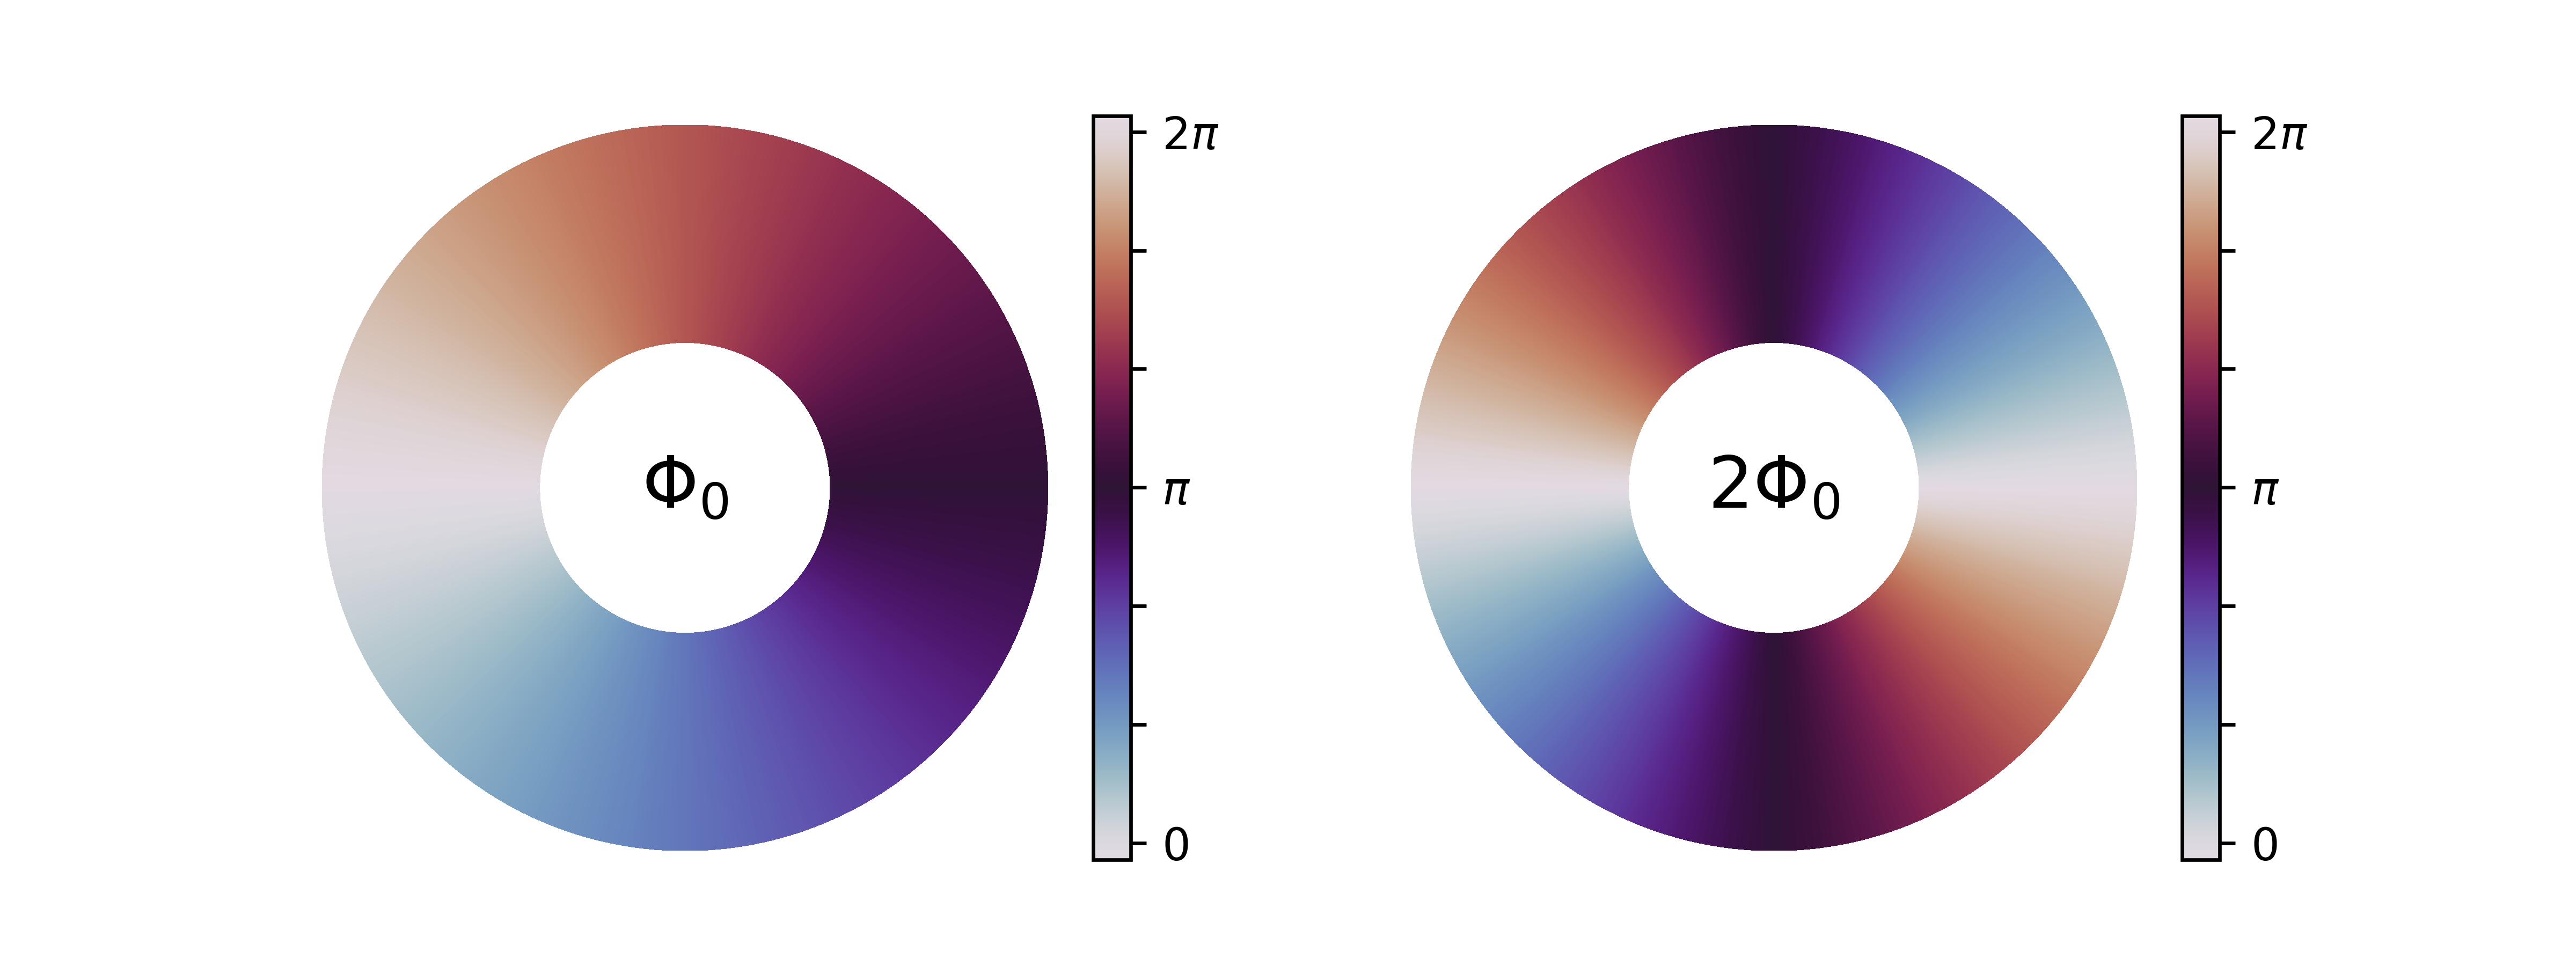
\includegraphics [width=1\textwidth] {coils}
	\caption{Распределение фазы волновой функции в сверхпроводящем кольце для различных значений магнитного потока.  }
	\label{img:coils}
\end{figure}
Квантование потока наглядно показывает, что во многих физических ситуациях, важных при описании сверхпроводниковых цепей, фаза оказывается очень тесно связанной с магнитным потоком. Экспериментально, квантование потока впервые наблюдалось в работе \cite{FluxQuant}  Связь между $\varphi$ и $\Phi$ носит примерно такой же характер, как связь между $n$ и полным зарядом $Q$ сверхпроводящего острова. Действительно, у сверхпроводящего острова к дискретному заряду $Q_n \!=\! n\cdot2e$ добавляется заряд $q\! = \!CV$, наведённый некоторым напряжением $V$ через какую-либо дополнительную ёмкость $C$, и полный заряд равен $Q\!=\!Q_n\!+\!q$. Похожим образом, <<внутренний>> поток $LI_m$, возникающий за счет индуктивного ответа в кольце на внешнее магнитное поле, складывается с внешним потоком $\Phi_{ext}$, и в результате получается дискретный <<полный>> поток $\Phi\!=\!n\Phi_0$. Но как создать какую-либо наведенную непрерывным образом фазу? Оказывается, что при использовании эффекта Джозефсона это становится возможным.
\subsection{Эффект Джозефсона: общие принципы}
Чтобы понять суть эффекта Джозефсона, рассмотрим два объемных сверхпроводника (берега), разделенных слоем диэлектрика. Будем называть такую систему джозефсоновским переходом (или SIS-переходом). Если этот слой достаточно толстый, то берега никак не связаны между собой. Начнем мысленно уменьшать толщину диэлектрического слоя, и рано или поздно возникнет туннельный эффект. Туннелировать могут как отдельные электроны (квазичастицы), так и куперовские пары, существующие независимо для каждого берега. Но куперовские пары имеют удвоенную массу по сравнению с квазичастичными возбуждениями. Поскольку вероятность прохожения барьера экспоненциально падает с ростом массы частицы, то при какой-то толщине $h_1$ барьер станет прозрачным только для квазичастиц, не пропуская куперовские пары. Квазичастицы не формируют конденсат, поэтому такое одноэлектронное туннелирование принципиально не будет отличаться от сходных процессов в нормальных металлах или полупроводниковых структурах. Туннельный ток будет зависеть от плотности состояний, и поэтому будет отличен от нуля только при $V\!>\!2\Delta$, что впервые наблюдалось в работе \cite{GiaeverGap}. Хоть процесс туннелирования куперовских пар весьма маловероятен, но тем не менее, барьер уже достаточно прозрачен, и можно сказать, что волновая функция отдельных электронов из одного берега частично проникает в другой. Продолжим уменьшать толщину диэлектрика. Оказывается, что при некоторой толщине $h_2\!<\!h_1$ возникает когерентность во всей электронной системе. Можно сказать, что куперовские пары образуются из электронов, принадлежащих двум разным металлам одновременно. Эти пары увлекаются в один или другой металл, а направление и  скорость их увлечения зависит от разности сверхпроводящих фаз между берегами. То есть, ненулевой сверхпроводящий ток возникает при $V\!=\!0$. Описанные процессы туннелирования схематично изображены на Рис.\:\ref{img:jj_tunn}. Из качественного рассмотрения может показаться, что одночастичный ток и ток конденсата должны возникать при одинаковой толщине барьера, но в действительности джозефсоновский ток наблюдается при меньшем нормальном сопротивлении, чем одночастичный. Это связано с влиянием тепловых флуктуаций, которые растут с увеличением $R$. Детальное описание можно найти в \cite{Barone}. Покажем, как этот ток зависит от разности фаз.
\begin{figure}
{\centering 
\hfill
\fontsize{22pt}{22pt}\selectfont
\def\svgwidth{3.5in}%
\input{images/JJ_disser.pdf_tex}
\hfill
}
\caption{SIS переход и различные процессы туннелирования через барьер.}
\label{img:jj_tunn}
\end{figure}
\subsection{Токо-фазовое соотношение}

%Прежде чем перейти к описанию эффекта Джозефсона, рассмотрим упрощенную модель электронной системы в сверхпроводнике в представлении зонной структуры. Прежде всего, имеется конденсат куперовских пар, то есть все пары находятся на одном энергетическом уровне, который можно выбрать за нулевой: $E=0$. Если разорвать пару, то возникает 2 квазичастичных возбуждения (электрона) c энергией $E>\Delta$, и если электрон видит частично прозрачный барьер, то он может протунеллировать из сверхпроводника. Также возможен процесс, когда уже имеющийся электрон с другой стороны барьера Вопрос о плотности состояний квазичастиц в зависимости от энергии может быть рассмотрен в теории БКШ, которая дает ответ:


Будем считать, что каждый из берегов имеет собственные состояния конденсата куперовских пар в нем, которые можно описать при помощи макроскопической волновой функции: $\Psi_R\! =\! \sqrt{\rho_R}e^{i\varphi_R}$ и $\Psi_L \!=\! \sqrt{\rho_L}
e^{i\varphi_L}$, где $\rho_R, \rho_L$ --- плотности частиц. Состояние всего конденсата можно искать в виде $\Psi = \Psi_L\ket{L}\!+\!\Psi_R\ket{R}$, что означает, что общий конденсат куперовских пар когерентно распределится так, чтоб минимизировать энергию всей системы. В базисе состояний $\ket{R}, \ket{L}$ гамильтониан системы можно записать в виде:
\begin{equation}
H = E_L\cdot \ket{L}\bra{L} + E_R\cdot \ket{R}\bra{R} + T\cdot\big[ \ket{L} \bra{R}+\ket{R}\bra{L}\big],
\end{equation}
где последний член описывает туннелирование системы как целого и означает, что потенциальный барьер достаточно прозрачен, и некоторые пары из конденсата могут состоять из электронов находящихся по разные стороны от барьера. Теперь можно решить уравнение Шредингера $i\hbar d\Psi/dt\! =\! H\Psi$, распадающееся на два уравнения для амплитуд $\Psi_L$~и~$\Psi_R$: 
\begin{align}
	i\hbar \frac{d\Psi_R}{dt} & =E_R\Psi_R+T\Psi_L, \nonumber \\
    i\hbar \frac{d\Psi_L}{dt} & =E_L\Psi_L+T\Psi_R.
    \label{eq: je_deriv}
\end{align} 
Подставим выражения для $\Psi_L$~и~$\Psi_R$, и получим ответ для плотности сверхпроводящего (джозефсоновского) тока через барьер $J_s={d\rho_R}/{dt}=-{d\rho_L}/{dt}$:
\vspace{-1pt}
\begin{equation}
J=\frac{2T}{\hbar}\sqrt{\rho_R \rho_L}\sin \varphi = J_c \sin \varphi,
\label{eq: cur-phase}
\end{equation}
где $\varphi = \varphi_L-\varphi_R$. Если считать $\rho_L$ и $\rho_R$ константами, что будет справедливо, например, в случае подключения к внешнему источнику тока, то величина $J_c$, называемая плотностью критического тока, зависит только от свойств перехода, а именно от типа сверхпроводника и ширины туннельного барьера. Микроскопическая теория дает следующее выражение для критического тока $I_c$ джозефсоновского перехода в случае нулевой температуры и одинаковых сверхпроводников с $\Delta_L=\Delta_R=\Delta$:
\begin{equation}
I_c = \frac{\pi \Delta}{2eR_n},
\end{equation}
где $R_n$ --- остаточное сопротивление на переходе при $T \ge T_c$. Впервые стационарный эффект Джозефсона наблюдался в работе \cite{StatJosephsonExp}.
Зависимость $J=J(\varphi)$ вида \eqref{eq: cur-phase} характерна не только для туннельного SIS-перехода, но и для многих других типов слабой связи (например, мост Дайема, SNS- и SSeS-переходы \cite{LikharevWL, CPhiR_review}). 
\subsection{Фазо-потоковое соотношение}
Выше было рассмотрено квантование магнитного потока в сплошном кольце. Рассмотрим, как меняется ситуация при прерывании кольца некоторым количеством SIS-переходов ($n$ штук), плоскости которых перпендикуляры плоскости кольца, см. Рис.\:\ref{img:ph-fl}. Будем считать, что внешнее магнитное поле невелико, и можно не учитывать его проникновение в область диэлектрика (которое приводит к необычным эффектам в переходах, см., например, \cite{Schmidt}, \S\:24). Выберем замкнутый контур $C$, пролегающий в глубине кольца, и запишем уравнение \eqref{eq:2GL} с учетом обращающегося в ноль мейсснеровского тока:
\begin{equation}
\label{eq: FFR}
\oint\displaylimits_{C}^{} \mathbf{A} d\boldsymbol{\ell} = \frac{\Phi_0}{2\pi}\oint\displaylimits_{C}^{}\nabla\varphi d\boldsymbol{\ell}
\end{equation}
Правая часть этого выражения содержит интеграл от градиента фазы вдоль контура. Однако, фаза не является непрерывной функцией, а скачкообразно меняется на переходах. Поэтому в таком виде вычислять интеграл нельзя. Разобъем контур $C$ на несколько отрезков кривой $A_iB_i, i=1,\ldots n$, таким образом исключая короткие отрезки контура $C$, лежащие внутри переходов, из контура интегрирования. Будем считать что левый интеграл при этом не изменяется:
\begin{equation}\label{eq:int_cAdl}
\oint\displaylimits_{C}^{} \mathbf{A} d\boldsymbol{\ell} = \sum_{i=1}^{n}\int\displaylimits_{A_i}^{B_i} \mathbf{A} d\boldsymbol{\ell},
\end{equation}
поскольку ширины переходов достаточно малы, а векторный потенциал не имеет никаких особенностей в коротких отрезках контура $C$, лежащих внутри переходов, так как токи и магнитные поля нулевые. Теперь вычислим правый интеграл как:
\begin{equation}
\label{eq:int_phi}
\begin{alignedat}{2}
\oint\displaylimits_{C}^{}\nabla\varphi d\boldsymbol{\ell} = \sum_{i=1}^{n}\int\displaylimits_{A_i}^{B_i}\nabla\varphi d\boldsymbol{\ell} = \sum_{i=1}^{n}\varphi_{B_i}-\varphi_{A_i} & = \\ =\varphi_{A_1} + \sum_{i=1}^{n-1}(\varphi_{A_{i+1}}-\varphi_{B_i}) - \varphi_{B_n} & = 2\pi k + \sum_{i=1}^{n}(\varphi_{A_{i+1}}-\varphi_{B_i}) = \\ 
& =2\pi k + \sum_{i=1}^{n}\delta\varphi_i,
\end{alignedat}
\end{equation}
В предпоследнем равенстве использовано условие однозначности волновой функции в виде $\varphi_{A_1} = \varphi_{A_{n+1}}-2\pi k$. Разности фаз на переходах обозначены как $\delta\varphi_i$. Подставляя \eqref{eq:int_cAdl} и \eqref{eq:int_phi} в \eqref{eq: FFR}, получаем искомое фазо-потоковое соотношение:
\begin{equation}
\label{eq: FFR_final}
\frac{2\pi\Phi}{\Phi_0} = 2\pi k + \sum_{i=1}^{n}\delta\varphi_i.
\end{equation}
Таким образом, поток в таком кольце не квантуется, но однозначно определяется разностями фаз на джозефсоновских переходах. Предположим, например, что джозефсоновские энергии переходов, входящих в кольцо, одинаковы и равны $E_J$, соответственно, равны и критические токи $I_c$. Тогда
\begin{equation}\label{eq: FFR_case}
\frac{2\pi}{\Phi_0}(\Phi_{ext}-LI_c\sin \delta\varphi)= 2\pi k + n\delta\varphi,
\end{equation}
и при заданных $L\text{ и }\Phi_{ext}$ можно найти такие $k \text{ и } \delta\varphi$, которые характеризуют разрешенные состояния системы. Если переходы различны, то разности фаз $\delta\varphi_i$ будут такими, чтобы токи через переходы $I_i=I_{ic}\sin\delta\varphi_i$ были одинаковыми. 
\begin{figure}
	\centering
		\fontsize{22pt}{22pt}\selectfont
		\def\svgwidth{3.5in}%
		\input{images/phase-flux2.pdf_tex}
	\caption{К выводу фазо-потокового соотношения.}
	\label{img:ph-fl}
\end{figure}
%\begin{figure}[ht] 
%	\centering
%	\includegraphics [width=1\textwidth] {coils_jj.png}
%	\caption{Распределение фазы волновой функции в сверхпроводящем кольце для различных значений магнитного потока.}
%	\label{img:coils_JJ}
%\end{figure}
\subsection{Энергия джозефсоновского тока. RSCJ-модель.}
Из уравнений \eqref{eq: je_deriv} можно получить следующее соотношение:
\begin{equation}
\frac{d\varphi}{dt} = \frac{2eV}{\hbar}.
\label{eq: dphidt}
\end{equation}
Таким образом, при конечном напряжении на контакте фаза начинает меняться с течением времени. Это так называемый нестационарный эффект Джохефсона, имеющий множество интересных применений, например генерация высокочастотного тока и создание стандарта напряжения. Используя полученное соотношение, можно рассчитать потенциальную (свободную) энергию, сосредоточенную в переходе:
\begin{equation}
\label{eq:EJ}  
E(\varphi) = \int_{0}^{t}I_sVdt = \int_{0}^{\varphi} I_c\sin \varphi' \frac{\hbar}{2e} {d\varphi'} = E_J(1-\cos\varphi).
\end{equation}
В последнем равенстве учтено что при нулевой фазе ток через переход не течет, и $E(0)=0$. Величина $E_J = {\hbar I_c}/{2e}$ называется \textit{джозефсоновской энергией} перехода. При малых значениях $\varphi$ энергия квадратично зависит от фазы: $E_J\approx E_J \varphi^2/2$, что дает возможность ввести эквивалентную линейную индуктивность перехода $L_{lin} = \Phi_0^2/2\pi I_c$. В более общем случае, джозефсоновская индуктивность зависит от фазы и определяется как $L_J = \Phi_0/(2\pi I_c \cos \varphi)$.
\begin{figure}[ht]
	{\centering
		\hfill
%		\subbottom[List-of-Figures entry][Туннельные процессы в SIS-переходе.\label{img:jj_tunnel}]{%
%			\input{images/JJ_disser.pdf_tex}}
%		\hfill
		\subbottom[List-of-Figures entry][RCSJ-модель перехода.]{%
			\input{images/RSCJ.pdf_tex}}
		\label{img:RCSJ}
		\hfill
		\def\svgwidth{2.2in}
		\subbottom[Частица в потенциале $U(\varphi)$.]{%
			\input{images/washboard.pdf_tex}}
		\label{fig: washboard}
		\hfill
	}
	\caption{RCSJ-модель джозефсоновского туннельного перехода.}
	\label{img:knuth_2}
\end{figure}

До сих пор мы рассматривали лишь энергию сверхпроводящего тока. Однако, для описания нестационарных процессов в реальных туннельных контактах такая модель недостаточна. Необходимо учитывать два дополнительных фактора: квазичастичное туннелирование и значительная емкость между двумя сверхпроводниками, неизбежно возникающая из-за малой толщины диэлектричекой прослойки (несколько десятков межатомных расстояний). Эти аспекты учитываются в феноменологической RCSJ-модели перехода, в которой параллельно с джозефсоновским элементом, энергия которого зависит от фазы согласно \eqref{eq:EJ}, включается эквивалентный резистор $R$, описывающий нормальное сопротивление квазичастичному току, и конденсатор $C$, см.\:Рис.\:\ref{img:RCSJ}. Полный ток через переход в такой схеме можно записать как:
\begin{align}
I &= I_C + I_J + I_R = \frac{\hbar C}{2e} \frac{d^2\varphi}{dt^2}+I_c\sin \varphi+ \frac{\hbar}{2eR}\frac{d\varphi}{dt}, \text{ отсюда получаем:}  \nonumber \\
0 & = m\frac{d^2\varphi}{dt^2} + f \frac{d\varphi}{dt} + \frac{d}{d\varphi}\big(E_J\cos \varphi+E_J\frac{ I}{I_c}\varphi\big), 
\end{align}
где введены обозначения $m=(\hbar/2e)^2 C$ и $f=(\hbar/2e)^2R^{-1}$. Полученное уравнение описывает динамику фазы в переходе как классическое движение частицы массой $m$ в жидкой среде с коэффициентом вязкости $f$ во внешнем потенциале стиральной доски $U(\varphi)=-E_J(\cos \varphi+I\varphi/I_c)$, что схематично отражено на Рис.\:\ref{fig: washboard}. Отметим некоторые характерные особенности динамики системы:
\begin{itemize}
	\item При отсутствии тока потенциал синусоидален, и частица локализуется в потенциальной яме, форма которой близка к параболической, и в этом случае может совершать малые колебания с частотой $\omega_p = (\sqrt{L_{lin}C})^{-1}$, называемой \textit{плазменной частотой перехода}. 
	\item Если увеличивать ток, то наклон потенциала растёт, потенциальная яма становится все более мелкой и пропадает. Частица начинает двигаться и будет разгоняться вдоль стиральной доски, пока не достигнет режима, в котором среднее значение $\langle V \rangle  \propto \langle d\varphi/dt \rangle$ постоянно и отлично от нуля. Характер её замедления при уменьшении тока (наклона) определяется параметром Маккамбера $\beta_c = \omega_p R C$, который показывает обратное число плазменных колебаний, которые система может совершить за время затухания $RC$ (при отсутствии тока).
	\item Если $\beta_c\ll1$, то при уменьшении тока частица практически не замедляется до тех пор, пока наклон не упадет практически до нуля. 
	\item Если $\beta_c\gg1$, то частица замедляется довольно значительно, так как трение играет существенную роль в её движении и скорость движения вдоль стиральной доски определяется средним наклоном. Полная остановка, однако, также произойдет лишь при $I=0$.
\end{itemize}
Перечисленные особенности находят подтверждение при измерении ВАХ переходов, полученных при фиксированном внешнем токе $I$, см., например, \cite{Schmidt}. 

Подведем итог классическому описанию джозефсоновского перехода. В зависимости от выбранного режима работы, такой переход может вести себя как нелинейный осциллятор, нелинейная индуктивность, зависящая от времени, либо демонстрировать еще более сложное поведение. Это делает его весьма интересным элементом даже с точки зрения классической схемотехники. Еще более нетривиальные эффекты возникают в том случае, если рассматривать разность фаз на переходе как квантовую степень свободы, которые мы кратко опишем далее. 
\section{Квантование электрических цепей}
\label{ch: Quant}

Как было сказано выше, при квантовом описании какой-либо сверхпроводящей системы число пар $\hat{n}$ на сверхпроводящем острове и фаза $\hat{\varphi}$ на этом острове могут рассматриваться как сопряженные переменные: $[\hat{\varphi}, \hat{n}]=i$. Возбуждения коллективной квантовой степени свободы при определенных условия оказываются самыми низкоэнергетическими (ниже 10 ГГц), и потому есть возможность экспериментально работать только с ними. В сверхпроводниках минимальная энергия одноэлектронного возбуждения не может быть меньше $2\Delta$, например, для алюминия имеем $2\Delta=3.52 k_b T_c\approx h\cdot80$ ГГц. Можно показать \cite{girvin2011circuit}, что частоты объемных плазменных колебаний попадают в терагерцовый диапазон, и поэтому их также можно исключить из рассмотрения. Фактически, мы будем иметь дело с бездисперсионными коллективными плазменными возбуждениями, и именно эти моды в итоге будут квантоваться. 
\subsection{Кубит. Двухуровневое приближение. Приближение вращающейся волны.}
\label{sec: qubit}
Простейшая квантовая система, например, спин $1/2$ в продольном магнитном поле, обладает одной степенью свободы и двумя собственными квантовыми состояниями. Обозначим состояния системы как $\ket{0}\equiv\begin{pmatrix} 1 & 0 \end{pmatrix}^{T} \text{и} \ket{1}\equiv\begin{pmatrix} 0&1 \end{pmatrix}^T$, а соответствующие собственные значения энергии как -$E_q/2$ и $E_q/2$. Тогда гамильтониан кубита записывается тривиально: $\hat{H}\!=\!\frac{-E_q}{2}\sz$. 

Согласно постулату квантовой механики, все возможные состояния кубита записываются как~$\ket{\psi}=\cos\frac{\theta}{2}\ket{0}+ 
e^{i\varphi}\sin\frac{\theta}{2}\ket{1}, 0 \le \theta \le \pi, 0 \le \varphi \le 2\pi $. Любая реальная система взаимодействует со своим окружением, поэтому состояния кубита необходимо описывать матрицей плотности:
\begin{equation}
\rho_q = \ket{\psi}\bra{\psi} =
\begin{pmatrix} \cos^2\frac{\theta}{2} & \cos\frac{\theta}{2}e^{-i\varphi}\sin\frac{\theta}{2}\\
\cos\frac{\theta}{2}e^{i\varphi}\sin\frac{\theta}{2}& \sin^2\frac{\theta}{2}
\end{pmatrix} = 
\begin{pmatrix} 1-\rho_{11} & \rho_{01}\\ \rho_{01}^*& \rho_{11}
\end{pmatrix}
\end{equation}
Последнее выражение можно обобщить и на случай смешанных состояний кубита, которые описывают статистический ансамбль. Поскольку матрицы Паули вместе с единичной матрицей составляют базис в пространстве матриц $2\times2$, то такую матрицу плотности можно записать в общем виде:
\begin{equation}
\rho_q = \frac{1}{2}(I+\vec{s}\cdot\vec{\sigma}),
\label{eq: rho_to_bloch}
\end{equation}
где $I$ --- единичная матрица, $\vec{\sigma}=\begin{pmatrix} \sigma_x & \sigma_y & \sigma_z \end{pmatrix}^{T}$ и
 $\vec{s}=\begin{pmatrix} s_x & s_y & s_z \end{pmatrix}^{T}$ --- трёхмерный вектор, называемый вектором Блоха. Для чистых состояний $\vec{s}=\begin{pmatrix} \sin\theta\cos\varphi & \sin\theta\sin\varphi & \cos\theta \end{pmatrix}^{T}$ можно представить как вектор из начала координат единичной длины, и все возможные положения конца этого вектора формируют единичную сферу --- сферу Блоха, см. Рис. \ref{img:bloch}.
\begin{figure}
 	\centering
 	\def\svgwidth{4in}
 	\input{images/Bloch_empty_3.pdf_tex}
 	\caption{Сфера Блоха. Точки на сфере соответствуют чистым состояниям кубита, точки внутри сферы --- смешанным состояниям.}
 	\label{img:bloch}
\end{figure} 

Квантовая двухуровневая система является простейшим объектом. В реальных экспериментах с СКЦ мы, как правило, работаем с многоуровневой системой. Но в некоторых физических ситуациях можно выделить два нижних уровня системы, и рассматривать систему внутри подпространства из основного и первого возбужденного квантовых состояний. 
Для этого необходимо делать двухуровневое приближение. 

Рассмотрим систему с собственными состояниями $\hat{H}_0\ket{n} = E_n\ket{n}$, под действием возмущения $\hat{V}(t)$. Учитывая поправку к собственным энергиям ${\tilde{E}_n}=E_n+\braket{n|\hat{V}|n}$, можно записать полный гамильтониан в виде:
\begin{equation}
\hat{H} = \sum_n\tilde{E}_n\ket{n}\bra{n} + \sum_{m \ne n}\textbf{}\ket{m}\bra{n}\braket{m|\hat{V}|n}. 
\end{equation} 
Оператор эволюции можно записать через повышающие и понижающие матрицы: $\hat{V} =   \sum_{m>n}\braket{m|\hat{V}|n}\hat{\sigma}_{mn}+\braket{n|\hat{V}|m}\hat{\sigma}_{nm}$. Тогда оператор эволюции возмущенной системы $U_0(t) = \exp(-\frac{i}{\hbar}(\tilde{E}_n\ket{n}\bra{n}))$ задаёт представление взаимодействия, гамильтониан в котором имеет вид:
\begin{equation}\label{eq: H_I}
\hat{H}_I = \sum_{m>n} e^{-{i}(\tilde{\omega}_n-\tilde{\omega}_m)t}\braket{m|\hat{V}|n}\hat{\sigma}_{mn} + \text{ c.c} 
\end{equation}
Если возмущение будет состоять из нескольких слагаемых, то соответствующие $\hat{H}_I$ могут не коммутировать, что сильно усложнит поиск аналитического решения для динамики системы и приведет к непоправимым последствиям. Однако, предположим, что $\hat{V}(t)\!=\!\hat{V}_0e^{i\omega t}$, где $\omega\!\approx\!\tilde{\omega}_{01}$. Тогда ясно, что наибольший вклад в оператор эволюции системы в представлении взаимодействия $\mathcal{T} \exp (-\frac{i}{\hbar}\int_0^t \hat{H}_I(t')dt')$ даёт слагаемое из \eqref{eq: H_I} с наиболее медленной зависимостью от времени. Все остальные члены дают интегралы от быстро осциллирующих функций, которые очень малы и не меняют характер динамики, заданной главным членом. Таким образом, мы можем сделать два приближения:
\begin{itemize}
	\item \textit{двухуровневое приближение} позволяет оставить в $H_I$ только члены $\braket{0|\hat{V}_0|1}\hat{\sigma}_{01} + e^{-2\omega t}\braket{1|\hat{V}_0|0}\hat{\sigma}_{10}$, пренебрегая переходами между остальными парами уровней, не попадающими в резонанс с возмущающим воздействием;
	\item \textit{приближение вращающейся волны} позволяет оставить только медленно меняющийся член $\braket{0|\hat{V}_0|1}\hat{\sigma}_{01}$.
\end{itemize}

Для того чтоб описывать СКЦ как кубит, необходимо, во-первых, уметь рассчитать её спектр в зависимости от параметров цепи и, во-вторых, уметь вычислить матричные элементы переходов под воздействием возмущений, например, внешнего электромагнитного поля. Теперь опишем общий формализм квантования цепи, а затем на некоторых примерах покажем, как осуществляются расчеты такого типа.
\subsection{Формальная процедура квантования цепи}	
Опишем общий подход к квантованию СКЦ \cite{vool2017introduction}. Будем рассматривать некоторую систему, состоящую из набора сверхпроводящих островов. Острова могут быть связаны взаимными емкостями и индуктивностями. Кроме того, некоторые из них могут образовывать джозефсоновскую связь. Поэтому, достаточно общим является представление такой системы в качестве электрической цепи, в которой имеются три типа элементов: емкости, индуктивности и джозефсоновские элементы (нелинейные индуктивности)\footnote[1]{Совсем недавно \cite{astafiev2012coherent} показана возможность создания т.н. центра когерентного квантового проскальзывания фазы, который является емкостным аналогом джозефсоновского перехода. Однако, создание квантовых цепей из таких элементов еще не вполне отработано. Их описание выходит за рамки данной работы.}. Как и в электротехнической цепи, в такой системе нужно подходящим образом выбрать некоторые независимые степени свободы, с помощью которых можно описать как классическую, так и квантовую динамику системы. Последовательность действий квантования системы состоит из следующих шагов:
\begin{enumerate}
\item Изобразим эквивалентную электрическую схему цепи. Схема будет состоять из N узлов (точек), связанных произвольным количеством элементов-двуполюсников, которые мы будем называть ребрами. Мысленно выделим емкостную и индуктивную части в общей схеме цепи. Поскольку любой реальный элемент имеет конечные размеры, и следовательно, паразитную емкость, то можно считать, что между каждой парой узлов включена емкость, и притом единственная. Среди всех узлов можно выделить \textit{активные} узлы, к которым подсоединены как емкостные, так и индуктивные элементы, и \textit{пассивные} узлы, к которым подсоединены только емкости.

\item Для каждого ребра введем величину $\Phi(t)=\int_{-\infty}^{t} v(t')dt'$, которую можно назвать магнитным потоком через ребро. Считается, что напряжение $v(-\infty)=0$ и плавно включается со временем. Тогда емкостную энергию можно записать как $C\dot{\Phi}^2/2$, что соответствует кинетической энергии частицы с кординатой $\Phi$. Для индуктивности эта величина в точности совпадает с запасённым в ней магнитным потоком, и индуктивная энергия $(\Phi-\widetilde{\Phi})^2/2L$ играет роль потенциальной энергии, где $\widetilde{\Phi}$ --- некоторый внешний поток. 
\item Выберем один из активных узлов емкостной подсистемы в качестве заземленного узла, и выберем только те емкости, которые единственным образом соединяют земляной узел со всеми остальными узлами подсистемы. Эти емкости составят \textit{остовное дерево} $T$. Тогда для любого другого узла $n$ можно ввести т.н. \textit{узловой поток} $\phi_n$, который равен сумме потоков всех емкостей, через которые нужно пройти от земляного узла до узла $n$. Связь между потоком через некоторое ребро $\Phi_b$ и потоками через узлы этого ребра $\phi_n, \phi_{n'}$ даётся соотношением:
\begin{equation}\label{eq: Phiphi}
\begin{aligned}
	\Phi_{b\in T} &= \phi_n-\phi_{n'}, \\
	\Phi_{b\notin T} &= \phi_n-\phi_{n'} + \widetilde{\Phi}_b,
\end{aligned}
\end{equation}
где внешний поток ${\Phi}_b$ учитывается в том случае, когда добавление ветви $b$ образует индуктивную петлю.
\item Используя соотношения \eqref{eq: Phiphi}, запишем полную энергию индуктивной и емкостной подсистемы через переменные $\vec{\phi}=(\phi_1\ldots\phi_N)^T$.  Энергия индуктивной подсистемы примет вид:
\begin{equation}
E_L(\vec{\phi}) = \frac{1}{2}{\vec{\phi}^{\mathsmaller T}} \mathbf{L^{-1}}\vec{\phi} + \sum_b \frac{\phi_n-\phi_{n'}}{L_b}\widetilde{\Phi}_b.
\end{equation}
Первое слагаемое представляет собой вклад в энергию непосредственно от индуктивностей. Матрица индуктивности $\mathbf{L}$ размера $(N-1)\!\times\!(N-1)$ симметричная и сконструирована следующим образом: недиагональные элементы $(i,j)$ равны $-\sum L_{ij}$, где $L_{ij}$ - все индуктивности, соединяющие узлы $i$ и $j$; диагональные же элементы равны сумме всех недиагональных элементов на соответствующей строке (или в столбце), взятой с противоположным знаком. Второе слагаемое --- это энергия каждой индуктивности, которая находится в ветви с внешним потоком $\widetilde{\Phi}_b$. Энергия емкостной подсистемы примет вид:
\begin{equation}
E_C(\dot{\vec{\phi}})= \frac{1}{2} {\dot{\vec{\phi}}^{\mathsmaller T}} \mathbf{C^{-1}} \dot{\vec{\phi}}
\end{equation}
где матрица емкости $\mathbf{C}$ строится аналогично матрице индуктивности.
\item Полученные выражения позволяют записать лагранжиан системы $\mathcal{L} = E_C-E_L$ и найти классические уравнения движения $\frac{d}{dt}\frac{\partial\mathcal{L}}{\partial\dot{\phi_n}}=\frac{\partial\mathcal{L}}{\partial{\phi_n}}$. Поскольку нас интересует квантовое описание системы, необходимо найти обобщенные импульсы $q_n = \partial\mathcal{L}/\partial{\dot\phi_n}$,  и записать гамильтониан $H = q_n\phi_n-\mathcal{L}$. Сколько независимых степеней свободы будет иметь система? Чтобы ответить на этот вопрос, необходимо заметить, что для любого пассивного узла $\partial \mathcal{L}/\partial{\phi_n}=0$, а поэтому $q_n$ является константой, и фактически, даннная степень свободы вырождена. Таким образом, если число активных узлов $P$, то полное число степеней свободы $P-1$.
\item Заменяя координаты (узловые потоки) и импульсы (узловые заряды) на сопряженные операторы $\phi\rightarrow\hat{\phi}$~и~$q\rightarrow\hat{q} = -i\hbar\frac{\partial}{\partial \phi}$, получаем гамильтониан квантовой цепи. Далее можно найти стационарные состояния, их энергии, матричные элементы переходов, и описать динамику системы.
\end{enumerate}
Далее мы рассмотрим некоторые базовые типы СКЦ. Как правило, они достаточно просты, и можно записать гамильтониан практически сразу, без предварительных шагов. Однако, следование общему формализму квантования необходимо для правильного описания более сложных цепей со многими степенями свободы. 
   
Базовые типы СКЦ, далее просто кубитов - это зарядовый кубит, фазовый кубит, потоковый кубит, трансмон и вч-СКВИД. Кратко опишем свойства каждого из этих кубитов.
\subsection{Зарядовый кубит}\label{charge_q}
	\begin{figure}[b]
		{ \raggedleft
			\hfill
			\def\svgwidth{2in}
			\fontsize{19pt}{19pt}\selectfont
			\subbottom[List-of-Figures entry][\label{img: CPB_scheme}]{%
				\input{images/CPB_qubit.pdf_tex}}
			\hfill
			\def\svgwidth{4in}
			\subbottom[\label{img: CPB_spectrum}]{%
				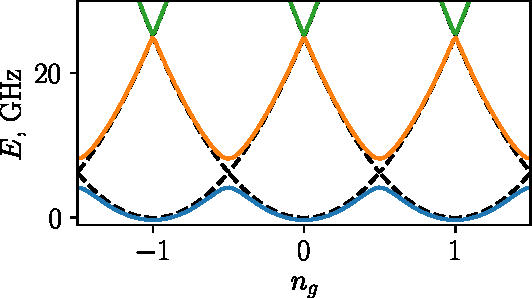
\includegraphics{images/CPB_spectrum.pdf}}
			
			\hfill
		}
		\caption[Схема зарядового кубита и его спектр.]{Зарядовый кубит: a) Эквивалентная схема кубита, б) Спектр кубита: три нижних энергетических уровня в зависимости от $n_g$. $E_C/h=\!=\!50 \text{ ГГц}, E_J/h\!=\!4\text{ ГГц}$. Пунктирная линия показывает классическую зарядовую энергию в отсутствие туннелирования.}
		\label{img: CPB}
		
	\end{figure}
Зарядовый кубит, или <<ящик>> для куперовских пар - это система, представляющая из себя джозефсоновский переход с энергией $E_J$, последовательно соединённый с емкостью. Эквивалентная схема такого кубита изображена на Рис.\ref{img: CPB}\subcaptionref*{img: CPB_scheme}. Образуется изолированный остров (выделен синим цветом), и если его емкость достаточно мала, то изменение числа куперовских пар на единицу сильно меняет энергию системы.  Введем зарядовую энергию конденсатора $E_C = 4e^2/C$; она включает в себя всю эффективную емкость острова, в т.ч. джозефсоновскую емкость. Также к острову подключен внешний источник, который может создавать наведенный заряд $n_g = C_gV_g/2e$.   Остовное дерево и земля выбираются тривиально, и понятно, что единственная степень свободы задается операторами фазы $\hat{\varphi}_1\!=\!2\pi/\Phi_0\!\cdot\!\hat{\phi}_1$ и заряда $\hat{n}_1\!=\!\hat{q}_1/2e$, далее индекс будет опущен за ненадобностью.~Гамильтониан системы имеет вид:
\begin{equation}
\hat{H}_{CPB} = \frac{E_C}{2}(\hat{n}-n_g)^2-E_J \cos \hat{\varphi}.
\end{equation}
Для нахождения спектра можно выбрать как фазовый базис, в котором $\hat{\varphi}\!=\!\varphi$, так и базис чисел куперовских пар (зарядовый базис), в котором $\hat{n}\!=\!n$. Начнем рассмотрение с зарядового базиса и выясним, как записать оператор $\cos\hat{\varphi}$. Заметим, что:
\begin{equation}
e^{i\hat{\varphi}}\ket{n} = e^{i\hat{\varphi}}\sum_n e^{in\hat{\varphi}}\ket{\varphi} = \ket{n+1},
\end{equation}
поэтому имеем:
\begin{equation}\label{eq: cosphi}
\cos \hat{\varphi} = \frac{1}{2}(e^{i\hat{\varphi}}+e^{-i\hat{\varphi}}) =
\frac{1}{2}\sum_n\Big(\ket{n+1}\bra{n} + \ket{n}\bra{n+1}\Big),
\end{equation}
где во втором слагаемом последнего выражения был сдвинут индекс суммирования $n \rightarrow n+1$. Гамильтониан можно записать в виде:
\begin{equation}
\hat{H}_{CPB} = \frac{E_C}{2}\sum_n(n-n_g)^2\ket{n}\bra{n}-\frac{E_J}{2} \sum_n\Big(\ket{n+1}\bra{n} + \ket{n}\bra{n+1}\Big).
\end{equation}
Получив его в такой форме --- диагональная часть плюс туннельный гамильтониан --- можно сразу сказать, как будет выглядеть собственные уровни энергии: в случае полуцелых $n_g$ два состояния с соседними $n$, вырождены. Новые собственные состояния сдвинуты на $\pm E_J/2$. Численно рассчитанный спектр изображен на Рис. \ref{img: CPB}\subcaptionref*{img: CPB_spectrum}. Сделаем двухуровневое приближение, то есть будем рассматривать подсистему из двух зарядовых состояний $\ket{0}$ и $\ket{1}$, и считать, что $n_g \approx 0.5$. Тогда гамильтониан примет вид: 
\begin{equation}
H_q = \frac{E_C}{2}(n_g-1/2)\sz-\frac{E_J}{2}\sx, 
\end{equation}
а новые собственные состояния системы можно записать через параметр $\theta = \arctan(\frac{2E_J}{E_C(n_g-1/2)})$ следующим образом: 
\begin{equation}
\begin{aligned}
\ket{g} & = \sin \frac{\theta}{2} \ket{0} + \cos \frac{\theta}{2} \ket{1}, \\
\ket{e} & = \cos \frac{\theta}{2} \ket{0} - \sin \frac{\theta}{2} \ket{1}
\label{eq: charge_e}
\end{aligned}
\end{equation}
Как и следовало ожидать, состояния максимально гибридизованы в окрестности $n_g\!=\!1/2$. 

Считается, что в пределе зарядового кубита $E_J < E_C$, то есть туннеллирование проявляется лишь между соседними зарядовыми состояниями. Отчасти исследование именно такого режима связано с тем, что зарядовый кубит --- исторически первый кубит, который был продемонстрирован в эксперименте \cite{nakamura1999coherent}. Для считывания используются такие методы, как джозефсоновский цикл квазичастичной генерации через дополнительный пробный барьер, подключенный к острову, а также одноэлектронный транзистор \cite{pashkin2009josephson}. Для такого считывания требуется, чтоб энергии зарядовых состояний при фиксированном $n_g$ сильно отличались друг от друга, то есть, ярко выраженный эффект кулоновской блокады. С этим связан и существенный недостаток зарядового кубита --- слишком высокая чувствительность к зарядовому шуму, влияющему на $n_g$. Различные паразитные двухуровневые системы в кремниевой подложке обладают электрическим дипольным моментом, влияющим на энергию кубита. Кроме того, попадание любой случайной квазичастицы на остров сильно сдвигает рабочую точку и делает длительную когерентную манипуляцию невозможной. В дальнейшем мы рассмотрим модификацию зарядового кубита с малой зарядовой энергией --- кубит-трансмон, работающий в так называемом пределе плоских зон, когда чувствительность к зарядовым шумам практически исчезает.
\subsection{Фазовый кубит}
Еще один тип кубитов, активно использовавшийся в 2000-х гг. --- фазовые кубиты \cite{martinis2009superconducting}. Фазовый кубит представляет собой смещенный постоянным током джозефсоновский переход. Точный контроль значения тока смещения $I$ позволяет хорошо контролировать глубину ямы в потенциале стиральной доски, см.~Рис. \ref{fig: washboard} и таким образом, регулировать число квантовых состояний, локализованных в яме. Пара нижних уровней и используется в качестве кубитной подсистемы. Управление осуществляется внешним высокочастотным током, подаваемым на переход. Считывание состояний \cite{steffen2006measurement} осуществляется при помощи дополнительной потоковой линии контроля: короткий импульс постоянного тока дополнительно наклоняет потенциал стиральной доски. Величина этого наклона подобрана таким образом, чтобы переход в состоянии $\ket{1}$ имел очень высокую вероятность протуннелировать через потенциальный барьер, который на время импульса становится значительно более прозрачным. В то же время, вероятность туннелирования состояния $\ket{0}$ должна быть исчезающе мала. Этого не так сложно добиться, учитывая тот факт, что согласно квантовой механике, в любой сколь угодно мелкой одномерной потенциальной яме имеется связанное состояние. Если туннелирование произошло, то джозефсоновский переход начинает движение вдоль стиральной доски, и на нём появляется ненулевое напряжение, и как следствие, высокочастотная компонента тока. Её можно обнаружить при помощи дополнительного считывающего пч-СКВИДa, что и делается в эксперименте. Как легко заметить, такое считывание разрушает кубит, и требуется конечное время для последующей инициализации в состоянии $\ket{0}$. Кроме того, шум тока смещения может вызывать значительное изменение потенциала, и как следствие, дефазировку кубита. Несмотря на имеющиеся недостатки, в работе с данными кубитами достигнут серьезный прогресс: были созданы 4-кубитные квантовые процессоры \cite{lucero2012computing}, реализующие простейшие квантовые алгоритмы, например, разложение на множители числа 15. В настоящий момент интерес к данному типу кубитов несколько уменьшился, однако, их исследование в достаточной мере способствовало развитию физики СКЦ.
 
\subsection{Потоковый кубит}
В зарядовом кубите, который мы рассмотрели ранее, реализуется суперпозиция состояний с разными числами куперовских пар на острове. Похожим образом можно создать суперпозицию состояний с различным значением магнитного потока в сверхпроводящей петле с включенными в неё джозефсоновскими переходами. Данная концепция была предложена в работе \cite{mooij1999josephson}, а кубит получил название <<кубит с незатухающим током>> и впоследствии упоминался упрощенно как \textit{потоковый кубит}. Схема потокового кубита с тремя джозефсоновскими переходами приведена на Рис.~\ref{img: flux_q}\subcaptionref*{img: fluxQ_scheme}. Обычно два перехода одинаковые, а площадь третьего перехода составляет $\alpha$ от площади больших переходов. Обычно выбирается $0\!<\!\alpha\!<\!1$. 
\begin{figure}[b]
	{ \raggedleft
		\hfill
		\def\svgwidth{3in}
		\fontsize{19pt}{19pt}\selectfont
		\subbottom[List-of-Figures entry][\label{img: fluxQ_scheme}]{%
			\input{images/3jj_qubit_ed.pdf_tex}}
		\hfill
		\subbottom[\label{img: flux_spectrum}]{%
			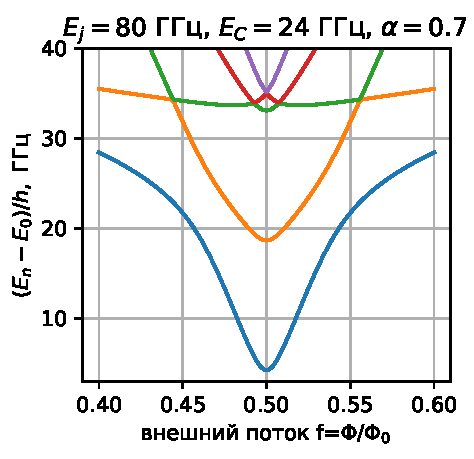
\includegraphics[width=0.5\textwidth]{images/3jj_spectrum_2.pdf}}
		
		\hfill
	}
	\caption[Схема потокового кубита и его потенциальная энергия.]{Потоковый кубит: a) Эквивалентная схема кубита, б) Спектр кубита: зависимости низших энергетических уровней в зависимости от $\Phi/\Phi_0$.}
	\label{img: flux_q}
	
\end{figure}

Запишем лагранжиан системы, используя операторы потока в узлах $\phi_i, i=\{1,2\}$ и их фазовые аналоги $\varphi_i=2\pi\phi_i/\Phi_0$:
\begin{multline}\label{eq: Lagr_flux}
{\mathcal{L}} = \frac{C}{2}
\begin{pmatrix}\dot{\phi}_1 &\dot{\phi}_2\\
	\end{pmatrix}
\begin{pmatrix}
	2 & -1\\ 
	-1 & \alpha+1 \\
\end{pmatrix}
\begin{pmatrix}\dot{\phi}_1\\\dot{\phi}_2\\\end{pmatrix}
%\Big[\frac{{\dot{\phi}}^2_1}{2}+ \frac{({ {\dot{\phi}}_2-{\dot{\phi}}_1})^2}{2} + \alpha\frac{{\dot{\phi}}_2^2}{2}\Big]
 + \\ + E_J\Big[ \cos(\varphi_1)+\cos(\varphi_2-\varphi_1+2\pi\frac{\Phi}{\Phi_0})+\alpha\cos(\varphi_2)\Big] 
\end{multline}
Введем обобщенные импульсы, которые в данном случае соответствуют числам куперовских пар на островах с потоками $\phi_1$ и $\phi_2$: 
\begin{equation}
\centering
\begin{aligned}
q_1 = 2en_1 & = \frac{\partial\mathcal{L}}{\partial\dot{\phi}_1} = {C}(2\dot{\phi}_1-\dot{\phi}_2) \\
q_2 = 2en_2 & = \frac{\partial\mathcal{L}}{\partial\dot{\phi}_2} = {C}((\alpha+1)\dot{\phi}_2-\dot{\phi}_1),
\end{aligned}
\end{equation}
которые для удобства дальнейших преобразований можно записать также в матричной форме: 
\begin{equation}
%\mathbf{n} = \frac{C}{2e}\mathbf{M\dot{\boldsymbol{\phi}}}, \
\mathbf{\dot{\boldsymbol{\phi}}} = \frac{2e}{C}\mathbf{M^{-1}}\mathbf{n},\ \text{где } \mathbf{M}=\begin{pmatrix}
2 & -1\\ 
-1 & \alpha+1 \\
\end{pmatrix}, \mathbf{n} = \begin{pmatrix}n_1\\n_2\\\end{pmatrix}, 
\mathbf{\dot{\boldsymbol{\phi}}} = \begin{pmatrix}\dot{\phi}_1\\\dot{\phi}_2\\\end{pmatrix}.
\end{equation}
Теперь можно записать гамильтониан системы $H(\mathbf{n}, \boldsymbol{\varphi}) = \mathbf{n^{\mathsmaller T}}\dot{\boldsymbol{\phi}}(\mathbf{n})-\mathcal{L}(\dot{\boldsymbol{\phi}}(\mathbf{n}), \boldsymbol{\varphi})$:
\begin{equation}\label{eq: Ham_flux}
H = \frac{E_C}{2}\mathbf{n^{\mathsmaller T}}\mathbf{M^{-1}}\mathbf{n}-E_J\Big[ \cos\varphi_1+\alpha\cos\varphi_2+\cos(\varphi_2-\varphi_1+2\pi\frac{\Phi}{\Phi_0})\Big]
\end{equation}
Первое слагаемое уравнения \eqref{eq: Ham_flux}, содержащее кинетическую энергию, выраженную через обезразмеренную матрицу емкости $\mathbf{M}$, применимо к любой системе, не содержащей экзотических элементов типа нелинейных емкостей, и может записываться практически сразу, минуя стадию построения лагранжиана. При этом операторы $n_i$ соответствуют числу куперовских пар на островах кубита. В данном случае мы считали также, что через замкнутую петлю кубита может быть приложен внешний магнитный поток $\Phi$. Из соотношения \eqref{eq: FFR_final} следует, что поток нужно включить в одно из слагаемых, описывающих джозефсоновскую энергию переходов. 

Получив выражение для гамильтониана системы, можно рассчитать энергетический спектр в зависимости от внешнего потока. Используя выражение \eqref{eq: cosphi}, можно записать гамильтониан в базисе зарядовых состояний:
\begin{equation}
\begin{aligned}
H = \frac{E_C}{2}&\sum_{n}\ket{n}_1\!\ket{n}_2\mathbf{M}^{-1}\bra{n}_2\!\bra{n}_1-\\\frac{E_J}{2}\Big[&\sum_{n}\ket{n+1}_1\!\ket{I}_2\!\bra{I}_2\bra{n}_1 +\ket{n}_1\!\ket{I}_2\!\bra{I}_2\!\bra{n+1}_1+\ldots\Big]
\end{aligned}
\end{equation}
где выражение типа $\ket{\cdot}_1\!\ket{\cdot}_2$ означает тензорное произведение векторов, соответствующих зарядовым состояниям островов 1 и 2. Кроме того, ряд слагаемых, входящих в джозефсоновскую энергию, опущен, поскольку они конструируются аналогично приведенному в формуле слагаемому с $\cos\varphi_1$. Такая запись гамильтониана позволяет перейти к численному решению проблемы. Выбирается некоторый базис зарядовых состояний от $-N$ до $N$ зарядов на острове, гамильтониан записывается как матрица размером $(2N+1)^2\times (2N+1)^2$, диагональные члены соотвествуют зарядовой энергии, а недиагонильные члены туннельного типа --- джозефсоновской энергии. После этого находятся собственные векторы и собственные значения гамильтониана, которые и дают спектр системы в зависимости от $\Phi$ в качестве параметра. Пример рассчитанного спектра приведен на Рис.\:\ref{img: flux_spectrum}. Можно заметить, что система обладает очень большим ангармонизмом: частота перехода 0-1 гораздо ниже частоты перехода 1-2. 

Также достаточно полезно рассчитать спектр и в фазовом базисе. Для этого зарядовые операторы необходимо записать в виде $n_1=-i\partial/\partial\varphi_1$. При этом уравнение на собственные энергии $H\ket{\Psi(\varphi_1, \varphi_2)}=E\ket{\Psi(\varphi_1, \varphi_2)}$ примет вид дифференциального уравнения в частных производных, которое можно решать численно при помощи некоторой разностной схемы. Один из вариантов такой схемы для сетки с шагом $h_1$ по фазе $\varphi_1$ и с шагом $h_2$ по фазе $\varphi_2$ имеет вид: 
\begin{equation}\label{eq: diff_scheme}
\newcommand{\pd}[2]{\frac{\partial#2}{\partial #1}}
\newcommand{\pdd}[2]{\frac{\partial^2#2}{\partial#1^2}}
\newcommand{\pmx}[3]{\frac{\partial^2#3}{\partial#1\partial#2}}
\newcommand{\vp}{\varphi}
\begin{aligned}
&\pdd{\vp_1}{\Psi(\varphi_1,\varphi_2)} = \frac{\Psi(\vp_1^{i-1}, \vp_2^i) -2\Psi(\vp_1^{i}, \vp_2^i) + \Psi(\vp_1^{i+1}, \vp_2^i)}{h_1^2}\\
&\pdd{\vp_2}{\Psi(\varphi_1,\varphi_2)} = \frac{\Psi(\vp_1^{i}, \vp_2^{i-1}) -2\Psi(\vp_1^i, \vp_2^i) + \Psi(\vp_1^{i}, \vp_2^{i+1})}{h_2^2}\\
&\pmx{\vp_1}{\vp_2}{\Psi(\varphi_1,\varphi_2)} = \pmx{\vp_2}{\vp_1}{\Psi(\varphi_1,\varphi_2)} = 
\pd{\vp_1}{}\frac{\Psi(\vp_1,\vp_2^{i+1}) - \Psi(\vp_1,\vp_2^{i-1})}{2h_2} = \\
&= \frac{\Psi(\vp_1^{i+1},\vp_2^{i+1}) - \Psi(\vp_1^{i+1},\vp_2^{i-1})}{4h_2h_1} - \frac{\Psi(\vp_1^{i-1},\vp_2^{i+1}) - \Psi(\vp_1^{i-1},\vp_2^{i-1})}{4h_2h_1} 
\end{aligned}
\end{equation}
Получившиеся собственные векторы покажут распределение собственных состояний кубита по различным фазам (т.е. состояниям с определенными фазами). Примеры такого распределения для основного состояния $\ket{g}$ и первого возбужденного состояния $\ket{e}$ приведены на Рис. \ref{img: 3jj_vs}. Видно, что эти состояния образуются за счет когерентного квантового туннелирования системы между двумя потенциальными ямами. 
\begin{figure}[h]\center
	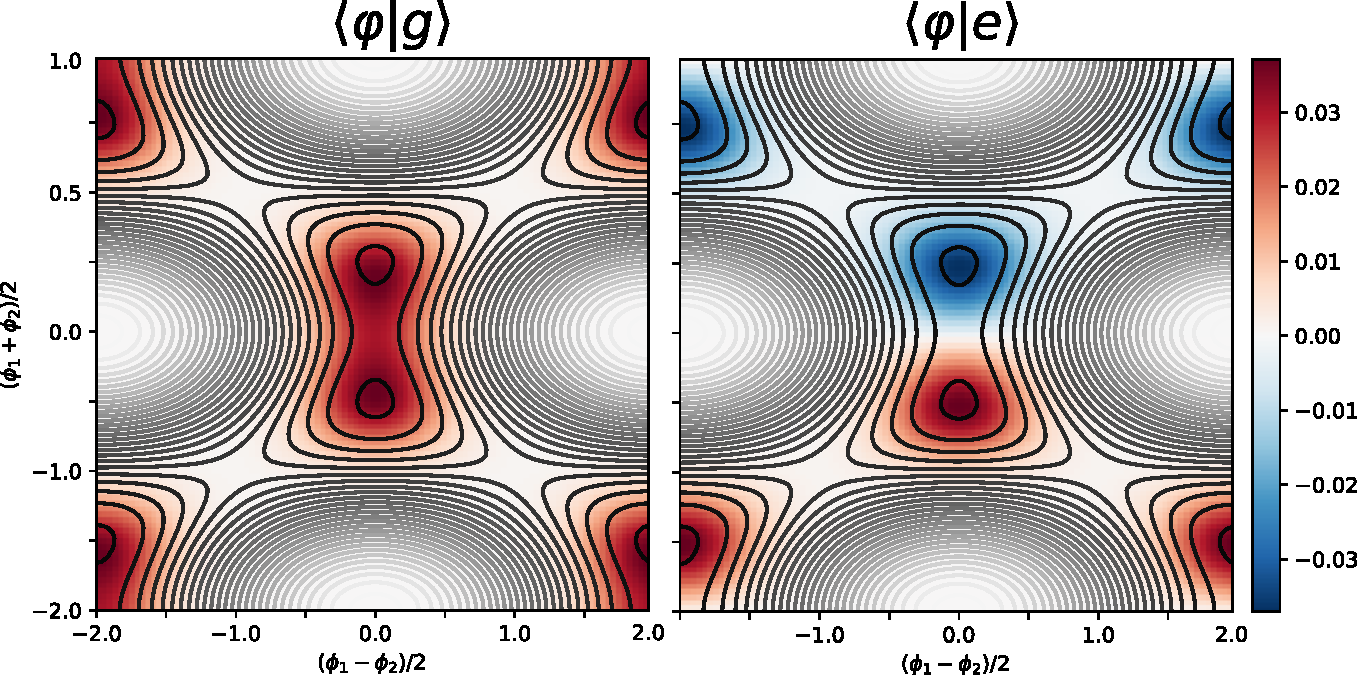
\includegraphics[width=0.95\textwidth]{images/3jj_vs.pdf}
	\caption{Волновая функция основного и первого возбужденного состояний потокового кубита при $\Phi=\Phi_0/2$. Линии уровня отображают потенциальную энергию.}
	\label{img: 3jj_vs}
\end{figure}
Высота барьера между двумя потенциальными ямами определяется параметром $\alpha$, и при $\alpha=0.5$ барьер исчезает. Поэтому данный параметр значительно влияет на собственные значения энергии и должен определяться достаточно точно, что может оказаться сложной задачей, особенно при использовании маленьких джозефсоновских переходов размерами порядка 200$\times$200 нм. Поэтому, как правило, воспроизводимость потоковых кубитов оказывается недостаточно хорошей. Также очевидно, что вне точки $\Phi=\Phi_0/2$ кубит восприимчив к потоковому шуму, что неизбежно будет вызывать дефазировку. Тем не менее, потоковый кубит остается достаточно интересен, прежде всего, за счет большого ангармонизма по сравнению с трансмоном, речь о котором пойдет ниже.  
\subsection{Трансмон} Рассмотренный в разделе \ref{charge_q} зарядовый кубит обладал многими несовершенствами. Попытки развития и соверщенствования даннго кубита привели к созданию кубита-трансмона. Трансмон --- это зарядовый кубит, шунтированный большой емкостью, у которого $E_C \ll E_J$~(обычно в 50 раз и более). Идея создания такого кубита впервые появилась в \cite{cottet2002implementation}, позднее было проведено подробное теоретическое исследование данных кубитов \cite{koch2007charge} и практически сразу же последовали первые эксперименты c трансмонами \cite{transmon}. Для того, чтобы проиллюстрировать необходимость такой модификации, приведем на Рис.~\ref{img: disp_vs_anh} относительный  aнгармонизм трансмона $(\omega_{10}-\omega_{21})/\omega_{10}$ и относительное изменение частот нижних переходов трансмона при изменении наведенного заряда $n_g$, то есть величину $|\omega_{i0}(n_g=e)-\omega_{i0}(n_g=0)|/\omega_{i0}(n_g=0)$ .  для различных значений отношения $E_C/E_J$. При уменьшении этого отношения уменьшается ангармонизм кубита.
\begin{figure}[h]\center
	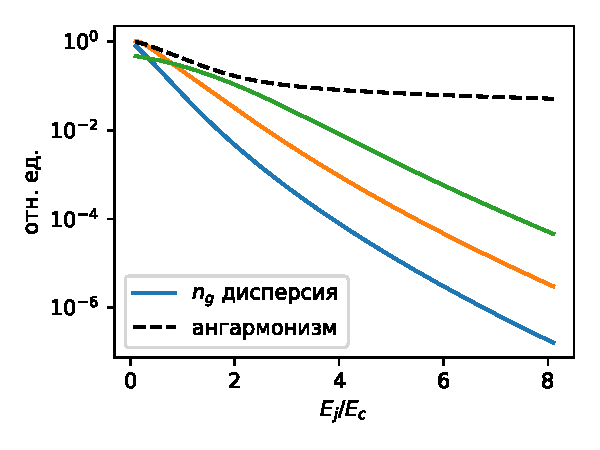
\includegraphics[width=0.75\textwidth]{images/disp_vs_anh.pdf}
	\caption{Изменение относительной зарядовой дисперсии для переходов 0-i трансмона и изменение ангармонизма основного перехода 0-1 в зависимости от отношения $E_J/E_C$. $E_C/h = 2$~ГГц}
	\label{img: disp_vs_anh}
\end{figure}
Для значений $E_C/E_J \approx 5$ кубит становится более похожим на гармонический осциллятор с относительно слабой нелинейностью в 5-10\% --- казалось бы, в таком эффекте нет никакой практической пользы. Но основным положительным эффектом от уменьшения $E_C/E_J$ является экспоненциально резкое падение зависимости энергетических уровней от $n_g$ --- так называемой зарядовой дисперсии. Особенно резко она уменьшается именно для низколежащих уровней, которые и используются на практике в качестве уровней кубита. Таким образом, удается достичь такого режима, когда ангармонизм еще достаточно большой и во многих ситуациях можно пренебречь верхними уровнями (или учесть их слабое влияние на динамику заселенности двух нижних уровней), и в то же время нежелательная зарядовая чувствительность практически подавлена. По этой причине для трансмонов характерны большие времена релаксации и декогеренции по сравнению как с зарядовыми, так и с потоковыми кубитами. Использование трансмонов при создании многокубитных схем оказалось весьма плодотворным, так как удалось разработать универсальные процессоры из 10 и более кубитов с полным контролем квантовых состояний. Однако, необходимо отметить, что во многих задачах трансмон нужно рассматривать как слабо нелинейный гармонический осциллятор, учитывая таким образом вклад верхних уровней. Например, при быстрых однокубитных операциях с трансмоном серьезную проблему представляют утечки заселенности кубита на второй возбуждённый уровень, которые необходимо предотвращать при помощи специальной коррекции управляющих импульсов. 

\subsection{вч-СКВИД}
Высокочастотный СКВИД - это прибор, представляющий собой джозефсоновский переход, шунтированный линейной индуктивностью $L$. Данный прибор изначально был предложен в 1965 г. для высокоточных измерений магнитного поля. Рассмотрим электрическую цепь вч-СКВИДа в квантовом режиме, см. Рис. Гамильтониан цепи имеет вид:
\begin{equation}
H = E_C \frac{n^2}{2} - E_J\cos(\phi - 2\pi\frac{\Phi}{\Phi_0}) + E_L\frac{\phi^2}{2}
\label{eq: rf_squid_ham}
\end{equation}
Зарядовая энергия возникает в результате внутренней емкости перехода и, возможно, некоторой паразитной емкости, которой обладает индуктивность из-за своего большого размера
Динамика фазовой переменной $\varphi$ аналогична динамике координаты квантовой частицы, помещенной в параболический потенциал, модулированный гармонической функцией. При этом масса частицы обратно пропорциональна емкости. Большая емкость локализует систему в одной из потенциальных ям, малая же емкость приводит к тому, что собственные состояния имеют достаточно большую неопределенность по фазе. Особый интерес представляет режим, когда $E_L \ll E_C < E_J$. В этом случае образуется несколько низколежащих потенциальных ям практически с одинаковой энергией, и соответствующие состояния гибридизуются. Получаемая при этом структура уровней сильно зависит от внешнего магнитного потока. Было показано, что в таком кубите возможно подавление квазичастичной релаксации, что было использовано для достижения времен жизни в несколько милисекунд. Однако, времена когерентности до недавнего времени оставались на уровне единиц микросекунд, и лишь в последнее время удалось повысить их до уровня кубитов-трансмонов \cite{grunhaupt2019granular}. 
\section{Микроволновая квантовая оптика}

В этом разделе будет обсуждаться квантовооптические эффекты, возникающие при взаимодействии отдельных сверхпроводниковых кубитов с микроволновым излучением. За исключением некоторых общих вопросов, преимущественно будет рассматриваться кубит, встроенный в волновод и сильно связанный с модами излучения в этом волноводе. Одной из особенностей, нехарактерных для <<природных>> атомов, является возможность эффективной передачи квантового состояния кубита в волновод. Это дает возможность собрать излучение от кубита и анализируя его, наблюдать фундаментальные явления, такие как резонансная флуоресценция, электромагнитно-индуцированная прозрачность, керровскую нелинейность одиночного атома и многие другие любопытные физические эффекты. 
\subsection{Кубит как открытая квантовая система. Релаксация и дефазировка}
\label{sec:Lind}
До сих пор мы рассматривали кубит как изолированную квантовую систему. Однако, в реальной физической ситуации кубит будет взаимодействовать с бесконечным количеством других квантовых систем. К примеру, значительное влияние на кубит оказывают так называемые \textit{двухуровневые дефекты} --- локализованные спины, возникающие из-за различных примесей или вакансий в кремниевой подложке. Такое окружение является практически неуправляемым и имеет бесконечно большое число степеней свободы. Поэтому составить и тем более решить уравнения движения для сложной системы <<кубит+окружение>> не представляется возможным. Необходимо использовать специально разработанные методы приближенного описания динамики относительно простой квантовой системы (в данном случае кубита) в произвольном окружении с макроскопически большим числом степеней свободы.

Принципиальный подход учета влияния окружения $B$ на квантовую систему $S$ состоит в следующем. Составная система $S+B$ описывается матрицей плотности $\rho(t)=\rho_B(t)\otimes\rho_S(t)$, которая меняется во времени по эволюционному закону. Если же мы хотим выделить и описать процессы, происходящие c $S$, то можно ввести некоторое динамическое отображение $V(t)$, преобразующее матрицу плотности по закону $\rho_S(t) = V(t)\rho_S(0)$. Разумеется, его можно получить из закона унитарной эволюции полной системы при помощи взятия следа по переменным окружения, но как было сказано выше, этот закон достаточно сложен, и скорее всего, неизвестен. Поэтому нужно получить явный вид $V(t)$ из некоторых предположений о характере взаимодействия системы и окружения.

Предположим, что система взаимодействует с окружением через некоторые операторы $\hat{A}_i$, то есть, гамильтониан взаимодействия содержит эти операторы, действующие на переменные системы, в составе тензорного произведения с какими-то операторами окружения. Для сверхпроводящих кубитов во многих случаях справедливо \textit{Марковское приближение}. Его суть в том, что окружение предполагается состоящим из макроскопически большого числа  взаимодействующих между собой квантовых систем. Поэтому можно считать корреляционное время окружения гораздо меньшим чем характерное время распада квантового состояния отдельного кубита. В этом приближении можно показать, что динамика системы описывается так называемым Линбладовским уравнением:
\begin{equation}
\frac{d}{dt}\rho_S = \mathcal{L}\rho_S(t) = -\frac{i}{\hbar}[H, \rho_S] + \sum_{i=0}^{N^2-1}\gamma_i\big( A_i\rho_SA^\dag_i -\frac{1}{2}\{ A_iA^\dagger_i, \rho_S\}\big)
\label{eq: Master_L}
\end{equation}
Второй член уравнения, представленный в виде суммы, называется \textit{диссипатором} и обозначается $\mathcal{D}\rho_S$. Операторы $A_i$ называются операторами Линблада для различных каналов распада системы, а $\gamma_i$ --- скорости распада системы по различным каналам, они имеют размерность обратного времени зависят от силы связи и от корреляционных функций окружения. Это уравнение дает возможность учесть различные механизмы влияния окружения на кубит. На примере одиночного кубита рассмотрим основные каналы распада квантового состояния. 

\subsubsection{Релаксация кубита}
Кубит с гамильонианом $\frac{\hbar \omega}{2}\hat{\sigma}_z$ может взаимодействовать с окружением посредством обмена квантами возбуждения, или энергией. Такое взаимодействие описывается гамильтонианом типа $H_{int} =\gamma(\hat{\sigma}_- \hat{a}^\dag + \hat{\sigma}_+ \hat{a})$. Используя \eqref{eq: Master_L}, получим выражение для диссипатора:
\begin{equation}
\mathcal{D}\rho_S(t) = \gamma\left( \sigma_- \rho_S(t) \sigma_+ -\frac{1}{2}\sigma_-\sigma_+\rho_S(t) -\frac{1}{2}\rho_s(t)\sigma_-\sigma_+ \right),
\label{eq: diss_ops}
\end{equation}
, или в явной матричной записи:
\begin{equation}
\mathcal{D}\rho_S = \frac{1}{2}\left[\begin{matrix}\gamma \left(- \rho_{z}{\left (t \right )} - 1\right) & \frac{\gamma}{2} \left(- \rho_{x}{\left (t \right )} + i \rho_{y}{\left (t \right )}\right)\\\frac{\gamma}{2} \left(- \rho_{x}{\left (t \right )} - i \rho_{y}{\left (t \right )}\right) & \gamma \left(\rho_{z}{\left (t \right )} + 1\right)\end{matrix}\right],
\label{eq: diss}
\end{equation}
где $\rho_x, \rho_y, \rho_z$ - компоненты блоховского вектора, введенного в \eqref{eq: rho_to_bloch}. Диагональные члены полученной матрицы показывают, что диссипация в первую очередь вызывает плавное <<перетекание>> заселенности состояния $\ket{1}$ в состояние $\ket{0}$, а недиагональные члены выражают тот факт, что любой канал распада состояния кубита со скоростью $\gamma$ также вносит дефазировку когерентностей кубита со скоростью $\gamma/2$. 
\subsubsection{Чистая дефазировка}
Еще один способ взаимодействия с окружением --- это влияние на резонансную частоту кубита, например, взаимодействие типа $H_{int} = \gamma_{\phi}\hat{a}^\dag\hat{a}\hat{\sigma}_z$. Это взаимодействие может реализовываться, например, в дисперсионном режиме модели Джейнса-Каммингса (см. ниже), когда перебросы двухуровневых систем в подложке эффективно вызывают сдвиг частоты перехода кубита. Более сложные механизмы дефазировки, связанные с вовлечением виртуальных двухфотонных процессов, описываются в \cite{Carmichael}. При этом результирующий диссипатор имеет вид:
\begin{equation}
\mathcal{D}\rho_S(t) = \frac{\gamma_\phi}{2}\left( \sigma_z\rho_S(t)\sigma_z - \rho_S(t)\right) = \frac{\gamma_\phi}{2}\left[\begin{matrix}0 & - \rho_{x}{\left (t \right )} - i \rho_{y}{\left (t \right )}\\-  \rho_{x}{\left (t \right )} + i \rho_{y}{\left (t \right )} & 0\end{matrix}\right]
\end{equation}
Недиагональные члены этого диссипатора вызывают затухание когерентностей кубита со скоростью $\gamma_\phi/2$, при этом никак не изменяются диагональные члены матрицы плотности. 
\subsection{Взаимодействие искусственного атома с внешним полем. Гамильтониан Джейнса-Каммингса.}
Рассмотрим, как одиночный естественный атом, расположенный в открытом пространстве, взаимодействует с падающим на него монохроматическим излучением. Будем работать в т.н. \textit{дипольном приближении}, которое предполагает, что длина волны электромагнитного поля гораздо больше размеров атома. Для случая сверхпроводникового кубита размерами 10-100 мкм это приближение выполняется для любых частот гигагерцового диапазона. Гамильтониан взаимодействия кубита и атома можно записать как $H_{int} = - \mathbf{d}\cdot\mathbf{E}$
где $\mathbf{d}$ --- оператор дипольного момента сверхпроводникового искусственного атома. Мы в данном случае предположили что атом связывается с напряженностью $\mathbf{E}$ электрического поля в точке расположения атома. Дипольный момент записывается как $\mathbf{d} = e \braket{g|\mathbf{r}|e}(\sigma_+ + \sigma_-)$, 
а стандартная процедура квантования поля дает для $\mathbf{E}$ следующее выражение: $$\mathbf{E} = \frac{1}{(2\pi)^3}\int\limits_{\omega}^{}\sqrt{\frac{\hbar\omega}{2\varepsilon_0}} \left(a_\omega^\dag+a_\omega\right).$$
После подстановки этих выражений в гамильтониан взаимодействия и учета гамильтонианов кубита и поля получается гамильтониан Раби:
\begin{equation}
H_R = \int\limits_{\omega}^{}\hbar \omega a^\dag_\omega a_\omega + \frac{1}{2}\hbar \omega_q\sigma_z + \hbar\int\limits_{\omega}^{}g_{\omega}(a_\omega^\dag + a_\omega)(\sigma_-+\sigma_+).
\end{equation}
Интегрирование здесь и ранее ведется по континууму мод, которые могут распространяться в волноводе. Если предположить, что константы связи $g_\omega$ достаточно малы по сравнению с частотой кубита, то справедливо приближение вращающейся волны. При переходе во вращающуюся систему отсчета с помощью унитарного преобразования $U_R =\exp\left({-i/2\hbar}(\omega_q\sigma_z+\omega a^\dag a)\right) $ слагаемые $a^\dagger\sigma_+$ и $a\sigma_-$ приобретут быстроосциллирующие множители $\exp\left( \pm(\omega+\omega_q)t\right)$. Эти множители практически не вносят вклада в динамику системы, поскольку:
$$\int_{}^{}e^{\pm in \omega t} dt=\frac{e^{\pm in \omega t}}{\pm in\omega}\propto \frac{1}{\omega}.$$
Отбрасывая эти слагаемые, получаем гамильтониан Джейнса-Каммингса:
\begin{equation}
H_{J-C} = \int\limits_{\omega}^{}\hbar \omega a^\dag_\omega a_\omega + \frac{1}{2}\hbar \omega_q\sigma_z + \hbar\int\limits_{\omega}^{}g_{\omega}(a_\omega^\dag\sigma_- + a_\omega\sigma_+).
\end{equation}
Отметим, что для распространения волны частотой 1-10 ГГц в копланарной проходной линии в случае, когда длина волны много превышает размер зазора, возможна только одна поляризация, при которой электрическое поле лежит в плоскости линии и направлено от центральной жилы к заземленным плоскостям (в течение одного полупериода колебаний). Все остальные моды, в том числе т.н. \textit{нечетные} моды, при которых ток течет по краям центральной жилы в противоположные стороны, а электрическое поле по обе стороны центральной жилы направлено в одну сторону, имеют гораздо более высокую частоту и не возбуждаются в интересующем нас диапазоне.   

\subsection{Режим сильной связи}
Понятие режима сильной связи можно применить к любым двум квантовым системам, которые взаимодействуют между собой. Для любых таких систем можно записать гамильтониан, который будет содержать часть, описывающую взаимодействие. Любое взаимодействие сводится к некоторой эффективной константе связи $g$, имеющей размерность энергии (частоты). При этом, помимо взаимодействия друг с другом, каждая из систем имеет некоторые потери энергии и/или дефазировку за счет взаимодействия со своим окружением, и эти потери тоже характеризуются некоторыми константами $\{\Gamma\}$. Для изучения совместной квантовой динамики систем наиболее интересным представляется случай, когда $g \gg \Gamma_i \in \{\Gamma\}$, то есть, сила взаимодействия значительно превосходит все возможные <<паразитные>> процессы, вызванные окружением и приводящие к потере квантового состояния в каждой из систем. В таком случае говорят, что эти системы находятся в режиме сильной связи. В случае атома, сильно связанного с электромагнитным полем внутри резонатора или проходной линии, возникает ряд интересных физических явлений, например, вакуумное Раби-расщепление 

Рассмотрим одномодовый случай модели Джейнса-Каммингса, который реализуется в случае связи кубита и резонатора. Покажем, что эта модель допускает точное решение. Естественный базис совместного гильбертова пространсва состояний кубита и резонатора $H_Q \otimes H_R$ можно составить из функций $\ket{\{e,g\}; n}, n \in \mathcal{N}$, в котором гамильтониан примет блочно-диагональный вид:
\begin{equation}
H_{JC}/\hbar=
\kbordermatrix{ \mathrm{state} &  \ket{e, n-1} & \ket{g, n} \\
	\ket{e, n-1} & \omega_q + (n-1)\omega & g \sqrt{n} \\
	\ket{g, n} & g\sqrt{n} & n\omega }
\end{equation}
Состояния гибридизуются попарно, и результирующие собственные энергии и состояния модели выглядят следующим образом:
\begin{equation}
\begin{split}
\ket{-,n} &= \cos \theta_n\ket{g,n}-\sin\theta_n\ket{e, n-1},\\
\ket{+,n} &= \cos \theta_n\ket{g,n}+\sin \theta_n \ket{e, n-1}, \text{где}\\
\theta_n &= \frac{1}{2}\arctan\Big(\frac{2g\sqrt{n}}{\Delta}\Big)
\end{split}
\end{equation}
\subsection{Эластичное и неэластичное рассеяние в копланарной линии}
В этом разделе будет рассмотрен процесс взаимодействия кубита и электромагнитный волны, распространяющейся в копланарной проходной линии вдоль оси $x$. Несмотря на кажущуюся простоту задачи, физическая суть происходящих при этом рассеянии явлений достаточно сложна. Будет показано, что есть принципиально различные компоненты рассеянного кубитом  сигнала: \textit{эластичная} и \textit{неэластичная} компонента. Для этого необходимо будет записать и решить уравнения динамики кубита с учетом релаксации в линию и проанализировать полученное стационарное решение. 
\subsubsection{Классическое поле в линии}   Начнем с классического описания взаимодействия некоторой системы, связанной с электромагнитным полем в линии. По сути, будет рассматриваться классический вариант \textit{теории входа-выхода}. Линия обладает погонной емкостью $c$ и погонной индуктивностью~$l$. Распространяющая волна создает некоторое распределение тока и напряжения вдоль линии. Уравнения, описывающие это распределение, называются \textit{телеграфными уравнениями} и записываются следующим образом:
\begin{equation}
\begin{split}
\frac{\partial V(x,t) }{\partial x} = -l\frac{\partial I(x,t)}{\partial t},\quad
\frac{\partial I(x,t) }{\partial x} = -c\frac{\partial V(x,t)}{\partial t}
\label{eq: telegr}
\end{split}
\end{equation}
Для удобства можно также разделить волны, распространяющиеся направо и налево в линии, сопоставив им соотвествующие напряжения $V^\rightarrow(x,t)$ и  $V^\leftarrow(x,t)$. Тогда полное напряжение и ток в линии записываются как:
\begin{equation}
\begin{split}
V(x,t) &= V^\rightarrow(x,t) + V^\leftarrow(x,t) \\
I(x,t) &= \frac{1}{Z}(V^\rightarrow(x,t) - V^\leftarrow(x,t)),
\label{eq: dirs}
\end{split}
\end{equation}
где $Z = \sqrt{l/c}$ - волновое сопротивление линии. Волновые уравнения принимают вид:
\begin{equation}
\begin{split}
	v\frac{\partial V^\rightarrow(x,t)}{\partial x} = -\frac{\partial V^\rightarrow(x,t)}{\partial t}, 
	v\frac{\partial V^\leftarrow(x,t)}{\partial x} = \frac{\partial V^\leftarrow(x,t)}{\partial t}, 
	\label{eq: telegr_dirs}
\end{split}
\end{equation}
где $v = 1/\sqrt{lc}$ - скорость распространения волны. 
Часто встречается случай, когда полубесконечная линия при $x>0$ замыкается на некоторую электрическую схему $S$, например, сверхпроводниковый кубит, расположенный в точке $x=0$. Тогда по отношению к этой схеме можно рассматривать возможные решения \eqref{eq: telegr_dirs} как входное и выходное напряжение, соответственно: $V^\leftarrow(t-x/v) \equiv V_{in}(t-x/v)$ и $V^\rightarrow(t+x/v) \equiv V_{out}(t+x/v)$. Используя \eqref{eq: dirs}, можно получить связь входного и выходного напряжений: 
\begin{equation}
V_{out}(t) = V_{in}(t) + ZI(0,t)
\label{eq: in_out}
\end{equation}
 Для того, чтобы эти уравнения полностью определяли ток и напряжение в линии, к ним необходимо добавить граничные условия, соответствующие реальной физической задаче.
\begin{itemize}
	\item  Если никакой системы нет и в точке $x=0$ линия претерпевает разрыв, то $I(0,t)=0$. Поэтому из \eqref{eq: in_out} следует идеальное отражение волны: $V_{out}(t) = V_{in}(t)$.
	\item Если отсутствует входной сигнал, то получаем $V_{out}(t) = ZI(0,t)$. Полубесконечная линия представляет из себя резистор с сопротивлением $Z$, подключенный к системе в качестве нагрузки. Измеряя напряжение $V_{out}(t)$, можно изучать динамику распада системы.
	\item В наиболее общем случае $I(0,t)\ne 0$, и схема инжектирует ток в линию. При 
	0
	необходимости можно рассчитать напряжение в точке $x=0$: $V(0,t) = 2V_{in}(t) + ZI(0,t)$.  	
\end{itemize}
\subsubsection{Взаимодействие кубита с классическим полем в линии}
Рассмотрим отдельный сверхпроводящий кубит, подключенный к бесконечной линии в точке $x=0$ при помощи связывающей емкости, см. Рис. ... . Применим к нему классическую теорию входа-выхода, изложенную также в~\cite{zagoskin2011quantum}. Это даст возможность получить аналитическое выражение для эластично рассеянного поля. 

Согласно схеме подключения кубита, появляется дополнительный узел электрической цепи, через который в линию будет втекать дополнительный ток из кубита. Таким образом, граничные условия можно записать в виде:
\begin{equation}
\begin{split}
	V(-0,t) &= V(+0,t) \\
	I(-0,t) + C_c\frac{d \langle \hat{V}_q \rangle }{dt} &= I(+0,t)
	\label{eq: bound_cond}
\end{split}
\end{equation}
Из граничных условий видно, что напряжение в точке $x\!=\!0$ меняется непрерывно, тогда как ток претерпевает скачок. Поэтому удобно рассмотреть ситуацию, когда распространяющаяся слева направо электромагнитная волна, амплитуда напряжения в которой равна $V_0$, претерпевает рассеяние на кубите. Запишем напряжение слева и справа от кубита в виде:
\begin{equation}
\begin{split}
V(x>0,t) &= t V_0 e^{-i(\omega t - k x)} \\
V(x<0,t) &= V_0 e^{-i(\omega t - k x)} - r V_0 e^{-i(\omega t + k x)} 
\label{eq: wave_scattering}
\end{split}
\end{equation}
Из этих уравнений с учетом условий \eqref{eq: bound_cond} получаем, что $t=1-r$. Подставляя \eqref{eq: wave_scattering} во второе уравнение в \eqref{eq: telegr} и интегрируя по координате $x$, получаем уравнения для тока:
\begin{equation}
\begin{split}
I(x<0,t) &= c V_0 \frac{\omega}{k}\cdot \big( re^{-i(\omega t + k x)} + e^{-i(\omega t - k x)}\big)\\
I(x>0,t) &= c V_0 \frac{\omega}{k} \cdot te^{-i(\omega t - k x)}
\end{split}
\label{eq: cur}
\end{equation}
Комбинируя эти выражения с уравнением для тока из \eqref{eq: bound_cond}, получим еще одно соотношение для коэффициентов прохождения и отражения:
\begin{equation}
1 + r = t + C_c\frac{k}{\omega cV_0}\frac{d \langle \hat{V}_q \rangle }{dt}e^{i\omega t}.
\end{equation}
Учитывая что $\omega/k=v=1/\sqrt{lc}$ - скорость распространения света в линии, получаем окончательное выражение для коэффициента отражения:
\begin{equation}
r = \frac{Z}{2V_0}C_c\frac{d\langle\hat{V}_q\rangle}{dt} e^{i\omega t}
\label{eq: r_derived}
\end{equation}  
\subsubsection{Основное квантовое уравнение кубита под действием резонансного поля}
Амплитудные коэффициенты отражения и прохождения достаточно удобны для их непосредственного измерения. Однако, полученное выражение \eqref{eq: r_derived} для $r$ и аналогичное выражение для $t$ непригодны для подгонки практических результатов, так как остается необходимым проанализировать операторный множитель и выразить его через измеряемые характеристики системы. 

Для простоты рассмотрим случай зарядового кубита в точке вырождения $\theta=\pi/2$ . Оператор напряжения на связывающем конденсаторе пропорционален заряду кубитного острова $\langle \dot{V_q} \rangle=\langle \dot{q} \rangle/C_\Sigma$, где $C_\Sigma$ - суммарная емкость между островом и землей. 
Согласно \eqref{eq: charge_e}, собственные состояния кубита в точке вырождения выражаются через зарядовые состояния как $\ket{g} = (\ket{0}+\ket{1})/\sqrt{2}$ и $\ket{e} = (\ket{0}-\ket{1})/\sqrt{2}$, поэтому в матричном виде можно записать:
\begin{equation}
\hat{q} = 
\begin{bmatrix}
\braket{e|\hat{q}|e} & \braket{e|\hat{q}|g} \\
\braket{g|\hat{q}|e} & \braket{g|\hat{q}|g}
\end{bmatrix} = e
\begin{bmatrix*}[r]
 0 &-1 \\
-1 & 0
\end{bmatrix*} + e
\begin{bmatrix*}[r]
1 & 0 \\
0 & 1
\end{bmatrix*}, 
\end{equation}
значит, $\braket{\dot{q}}=e\frac{d\braket{\sigma_x(t)}}{dt}$. Усреднение в данном случае означает математическое ожидание оператора по состоянию кубита. Поскольку кубит бесконечно долго взаимодействует с непрерывной волной и при этом одновременно излучает в линию, то логично предположить, что эти процессы компенсируют друг друга. Поэтому с течением времени кубит должен оказаться в некотором стационарном состоянии, которое можно определить из условия $\dot{\rho} = 0$. Для нахождения $\langle\sigma_x(t)\rangle$ необходимо записать и решить основное квантовое уравнение для кубита. Гамильтониан взаимодействия зарядового кубита с напряжением в линии имеет вид:
\begin{equation}
H_{int} = C_cV\hat{V}_q = \frac{C_c}{C_\Sigma}V_0\cos(\omega_d t + \varphi)\braket{g|\hat{q}|e}\sigma_x,
\label{eq: Hint_class}
\end{equation} 
причем для зарядового кубита $\braket{g|\hat{q}|e} = e$. Для случая трансмона \cite{koch2007charge} собственные состояния являются суперпозициями большого числа зарядовых состояний, поэтому рассчитать матричный элемент несколько сложнее: 
\begin{equation}
\braket{g|\hat{q}|e} = \frac{2e}{\sqrt{2}}\left(\!\frac{E_J}{E_C}\!\right)^{\!\frac{1}{4}}.
\end{equation}
Вводя обозначение для емкостного коэффициента эффективности связи  $\beta = C_c/C_\Sigma$ и Раби-частоты $\Omega = \beta V_0\braket{g|\hat{q}|e}/\hbar$, получаем из \eqref{eq: Hint_class} окончательное выражения для гамильтониана взаимодействия. Полный гамильтониан примет вид:
\begin{equation}
H = H_q + H_{int} = -\frac{\hbar \omega_q}{2}\hat{\sigma}_z+ \hbar\Omega\cos(\omega_d t + \varphi)\hat{\sigma}_x
\label{eq: H_int_class_final}
\end{equation} 
Чтобы вывести основное квантовое уравнение, сначала воспользуемся приближением вращающейся волны, описанным в разделе \ref{sec: qubit}. Преобразуя $H$ при помощи унитарного преобразования $U=\exp(-i\omega_d\sz/2\hbar)$, имеем:
\begin{equation}
\label{eq: Hrot}
H_{rwa}=UHU^\dagger-iU\dot{U}^\dag \approx \frac{\hbar}{2}\left[\begin{matrix}- \omega_d + \omega_q & \Omega e^{- i \varphi}\\\Omega e^{i \varphi}  & \omega_d - \omega_q\end{matrix}\right],
\end{equation}
где были отброшены быстро осциллирующие члены $\Omega e^{\pm i \varphi} e^{\pm2 i \omega_d t}$ в недиагоальных слагаемых. Используя этот гамильтониан, можно записать основное квантовое уравнение, представляющее собой уравнение Лиувилля-фон Неймана для эволюции квантовой системы, описывающейся оператором плотности и линбладовский член, характеризующий взаимодействие с внешней средой:
\begin{equation}
\frac{d\rho}{dt} = -\frac{i}{h}[H_{rwa}, \rho] + \mathcal{L}.
\label{eq: QLiouv}
\end{equation}
Линдбладовский член, который включает в себя релаксацию $\Gamma_1$ и дефазировку $\gamma_\phi$, описанные ранее в разделе \ref{sec:Lind}, имеет следующий вид:
\begin{equation}
\mathcal{L} = \left[\begin{matrix}-\Gamma_1 \left(\rho_{z}+1\right) & -\Gamma_1 \left( \frac{\rho_{x}}{2}-\frac{i \rho_{y}}{2}\right) - \gamma_{\phi} \left(\rho_{x} - i \rho_{y}\right)\\-\Gamma_1 \left( \frac{\rho_{x}}{2} + \frac{i \rho_{y}}{2}\right) - \gamma_{\phi} \left(\rho_{x} + i \rho_{y}\right) & \Gamma_1 \left(\rho_{z} + 1\right)\end{matrix}\right]
\end{equation}
После преобразований уравнение запишется в следующем виде:
\begin{equation}
\label{eq: Bloch}
\dot{\vec{\sigma}}{\left(t\right)} = \mathbf{M}\vec{\sigma}{\left(t\right)} + \vec{b}, 
\end{equation}
где введены обозначения:
\begin{equation}
\vec{\sigma}(t) = \left[\begin{matrix}\rho_x(t)\\\rho_y(t)\\\rho_z(t)\end{matrix}\right], \:	
\mathbf{M}=\left[\begin{matrix}- \frac{\Gamma_1}{2} - \gamma_{\phi} & \omega_d - \omega_q & \Omega \sin{\varphi}\\- \omega_d + \omega_q & - \frac{\Gamma_1}{2} - \gamma_{\phi} & - \Omega \cos{\varphi }\\- \Omega \sin{\varphi } & \Omega \cos{\varphi} & - \Gamma_1\end{matrix}\right], \:\vec{b} = \left[\begin{matrix}0\\0\\- \Gamma_1\end{matrix}\right].
\end{equation}
Уравнения \eqref{eq: Bloch} называются \textit{уравнениями Блоха} и полностью описывают динамику двухуровневой системы, связанной с окружением и находящейся под действием внешнего электромагнитного поля. 
\subsubsection{Динамика состояния кубита под действием поля}
Уравнения Блоха \eqref{eq: Bloch} могут быть решены точно. Для получения решения воспользуемся подстановкой $\vec{\sigma}(t) = e^{\mathbf{M}t}\vec{v}(t)$, которая преобразует уравнение \eqref{eq: Bloch} к виду:
\begin{equation}
e^{\mathbf{M}t}\dot{\vec{v}}(t) = \vec{b},
\end{equation}откуда формальным интегрированием получаем: $\vec{v} = \mathbf{-M^{-1}}e^{-\mathbf{M}t}\vec{b} + \vec{v}_0$. Константа интегрирования $\vec{v}_0$ зависит от начального состояния атома: $\vec{\sigma}_0 =  -\mathbf{M^{-1}}\vec{b} + \vec{v}_0$. С учетом этого получаем окончательное выражение:
\begin{equation}
\vec{\sigma}(t) = -\mathbf{M^{-1}}\vec{b} + e^{\mathbf{M}t}\left(\vec{\sigma}_0 + \mathbf{M^{-1}}\vec{b}\right)
\end{equation}
Окончательные выражения, описывающие динамику атома, достаточно громоздки. Выпишем решение для частного случая $\varphi=0, \delta\omega=\omega_q - \omega_d = 0$:
\begin{equation}
\textstyle
\frac{1}{2 \left(2\Omega ^2+2 \gamma _{\varphi } \Gamma _1+\Gamma _1^2\right) \Omega _r}
\left[\begin{smallmatrix}
0 \\
4 \Omega  \Gamma _1 \Omega _r+e^{-\Gamma_r t } \Omega \left[  
	\left(4 \Omega ^2+2 \gamma _{\varphi } \Gamma _1-\Gamma _1^2\right)\sin \Omega _rt-4  \Gamma _1 \Omega _r\cos \Omega_rt\right] \\
-2 \Gamma _1 \left(2 \gamma _{\varphi }+\Gamma _1\right) \Omega _r-e^{-\Gamma_r t } \Omega
	^2 \left[\left(2 \gamma _{\varphi }+3 \Gamma _1\right)\sin \Omega _r t +4  \Omega _r \cos \Omega _r t\right] \\ 
\end{smallmatrix}
\right]
\label{eq: dyn_sol}
\end{equation}
Можно заметить, что динамика имеет вид осцилляций, которые затухают со временем, см.~Рис. \ref{img: Rabi_dyn_res}. Они называются осцилляциями Раби. 
\begin{figure}[t]
	\centering
	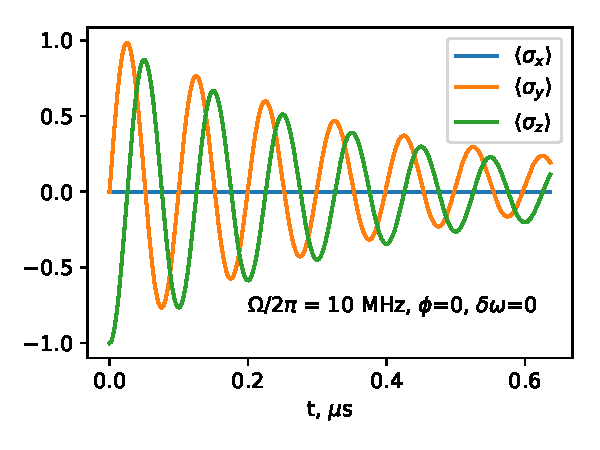
\includegraphics[width=0.6\textwidth]{images/Rabi_res.pdf}
	\caption[Динамика состояния кубита под действием внешнего поля в случае резонанса]{Динамика среднего состояния кубита под воздействием поля. Компоненты блоховского вектора $\{\braket{\sigma_x(t)}, \braket{\sigma_y(t)}, \braket{\sigma_z(t)}\}$ в явном виде заданы выражением $\eqref{eq: dyn_sol}$.}
	\label{img: Rabi_dyn_res}
\end{figure}

Отметим некоторые особенности полученного решения. Во-первых, частота Раби осцилляций определяется как $\Omega_r = \sqrt{\Omega^2-(\Gamma_1-2\gamma_\varphi)^2/16}$, и практически совпадает с $\Omega$ в случае достаточно сильного драйва. Затухание Раби-осцилляций определяется как $\Gamma_r = \frac{1}{4}\left(2 \gamma _{\varphi }+3 \Gamma _1\right) = \left(\Gamma_1 + \Gamma_2\right)/2$. Этот результат качественно объясняется тем, что примерно половину времени кубит проводит на экваторе сферы Блоха, где он существенно подвержен влиянию дефазировки, а другую половину кубит имеет положительную проекцию на ось $z$, и соответственно, подвержен влиянию затухания.
В случае $\delta\omega \ne 0$ окончательный ответ еще более громоздкий, поэтому мы не приводим уравнения, описывающие динамику в этом более общем случае. Динамика кубита при ненулевой отстройке изображена на~Рис.~\ref{img: Rabi_dyn_det} и \ref{img: Bloch_Rabi_dyn_det}. Заметим, что общий характер колебаний остается примерно таким же, что и в случае $\delta\omega=0$, однако, заметно меняется конечное состояние кубита, в котором он оказываеся после осцилляций - стационарное состояние. Получим явное выраджение, описывающее стационарное состояние кубита.
\begin{figure}[t]
	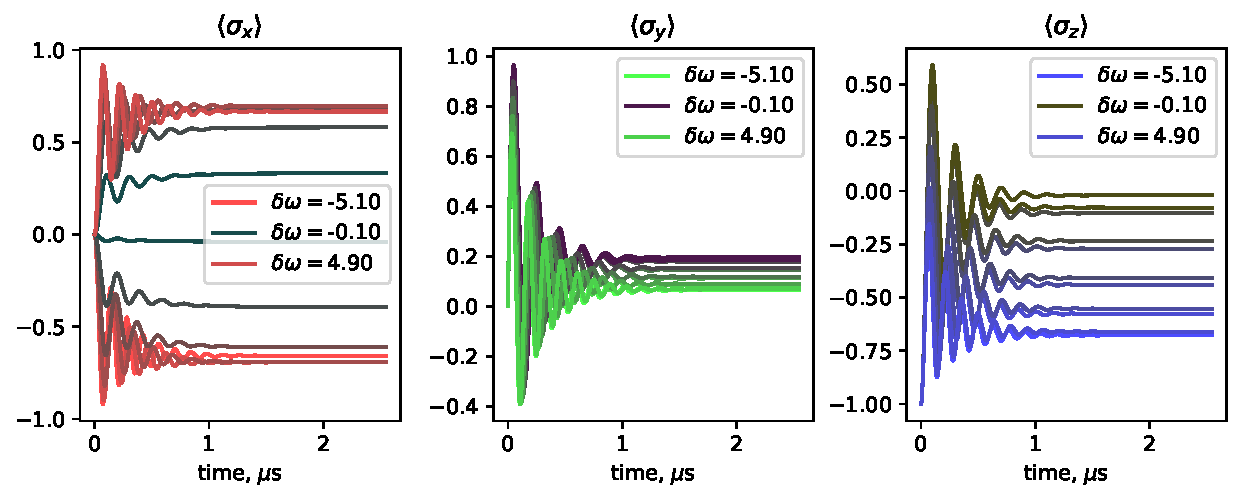
\includegraphics[width=0.98\textwidth]{images/Rabi_det_2.pdf}
	\caption[Динамика состояния кубита под действием внешнего поля: случай ненулевой отстройки]{Динамика компонент блоховского вектора $\vec{\sigma}(t)$ для $\Gamma_1=0.5, \gamma_\varphi=0.1, \Omega = 10$~МГц. Линии на каждом из графиков соответствуют значениям $\delta\omega=[-5.1,4.9]$~МГц }
	\label{img: Rabi_dyn_det}
\end{figure}
\begin{figure}[h]
	\centering
	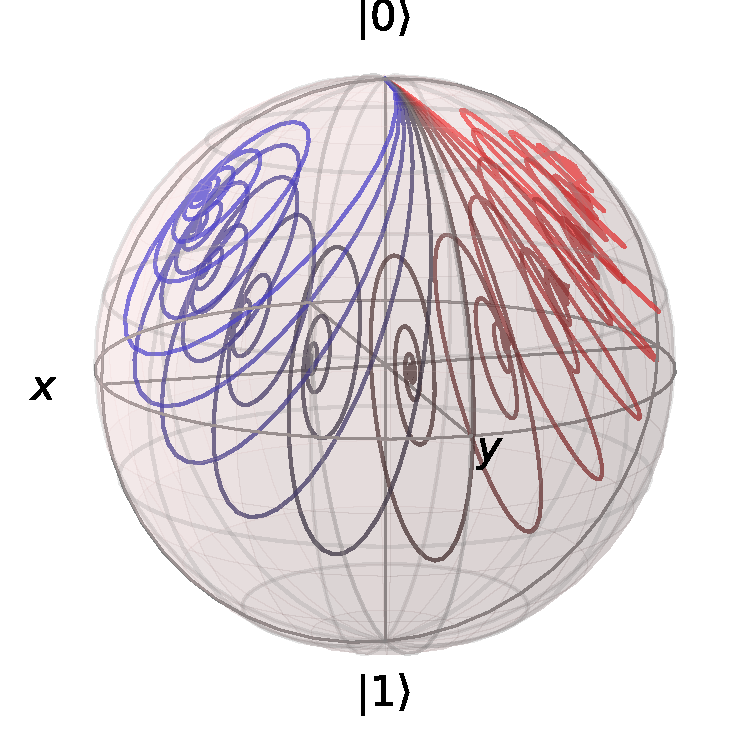
\includegraphics[width=0.65\textwidth]{images/Bloch_rabi_det.pdf}
	\caption[Динамика состояния кубита под действием внешнего поля на сфере Блоха]{Динамика состояния кубита при ненулевой отстройке внешнего драйва, изображенная на сфере Блоха. Кривые построены при тех же параметрах, которые использованы для Рис. \ref{img: Rabi_dyn_det}.}
	\label{img: Bloch_Rabi_dyn_det}
\end{figure}
\subsubsection{Стационарное решение уравнений Блоха}
Поскольку кубит постоянно взаимодействует с полем, время от времени обмениваясь энергией или информацией с внешней средой, то можно предположить, что временная динамика матрицы плотности, которая, строго говоря, описывает распределение эволюций одинаковых систем, через достаточно долгое время придет к некоторому стационарному значению $\vec{\sigma}_{st}$. Это легко проверить, положив в уравнениях \eqref{eq: Bloch}  $\dot{\vec{\sigma}}(t)=0$, что делает дифференциальные уравнения алгебраическими. Полагая $\varphi=0$ (что задает вращение вокруг оси $x$) и решая уравнения относительно компонент блоховского вектора, находим:
\begin{multline}
\rho_{x} = \frac{4 \Gamma_{1} \Omega \delta\omega}{4 \Gamma_{1} \delta\omega^{2} + \Gamma_{1} \left(\Gamma_{1} + 2 \gamma_{\varphi}\right)^{2} + 2 \Omega^{2} \left(\Gamma_{1} + 2 \gamma_{\varphi}\right)},\\\rho_{y} = \frac{2 \Gamma_{1} \Omega \left(\Gamma_{1} + 2 \gamma_{\varphi}\right)}{4 \Gamma_{1} \delta\omega^{2} + \Gamma_{1} \left(\Gamma_{1} + 2 \gamma_{\varphi}\right)^{2} + 2 \Omega^{2} \left(\Gamma_{1} + 2 \gamma_{\varphi}\right)},\\ \rho_{z} = - \frac{\Gamma_{1} \left(4 \delta\omega^{2} + \left(\Gamma_{1} + 2 \gamma_{\varphi}\right)^{2}\right)}{4 \Gamma_{1} \delta\omega^{2} + \Gamma_{1} \left(\Gamma_{1} + 2 \gamma_{\varphi}\right)^{2} + 2 \Omega^{2} \left(\Gamma_{1} + 2 \gamma_{\varphi}\right)},
\label{eq: stat_sol}
\end{multline}
где введено обозначение $\delta\omega=\omega_d-\omega_q$.
\begin{figure}[h]
	{ \raggedleft
		\hfill
		\def\svgwidth{2.5in}
		\fontsize{19pt}{19pt}\selectfont
		\subbottom[\label{img: bloch_stat1}]{%
			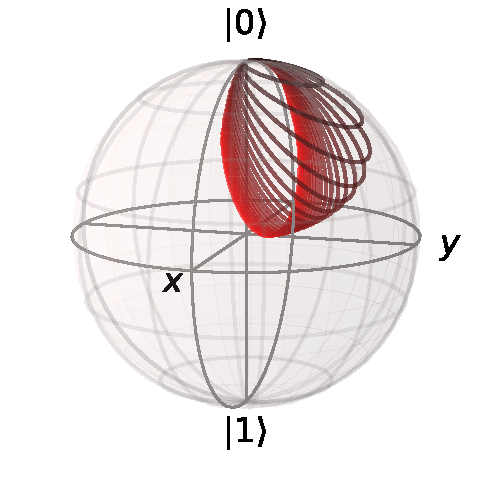
\includegraphics{images/bloch_stat1.pdf}}
		\hfill
		\def\svgwidth{2.5in}
		\subbottom[\label{img: bst2}]{%
			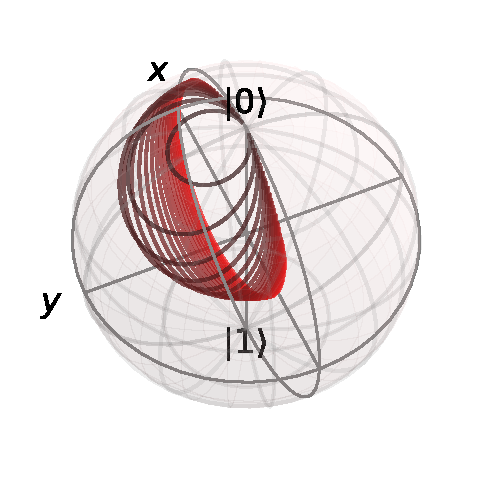
\includegraphics{images/bloch_stat2.pdf}}
		
		\hfill
	}
	\caption[Стационарное состояние кубита, вращаемого электромагнитным полем.]{Стационарное состояние \eqref{eq: stat_sol} кубита под воздействием поля, изображенное на сфере Блоха. Различные линии соответствуют значениям $\Omega=[0,10]$, $\Gamma_1=2, \gamma_\varphi=0 $~МГц. Каждая линия соответствуют изменению $\delta\omega=[-10,10]$~МГц. Панели а) и б) изображают одни и те же линии под различными ракурсами. Отметим, что эти линии образованы множеством точек, к которым приходит кубит после динамики, изображенной на~Рис. \ref{img: Bloch_Rabi_dyn_det} \label{img: bloch_stat}}
	
\end{figure}
Стационарные состояние в зависимости от параметров $\Omega, \Gamma_1, \gamma_\varphi$ изображено на Рис.~\ref{img: bloch_stat}. В случае $\Omega\!\ll\!\Gamma_1$ стационарное состояние приближено к состоянию $\ket{0}$, поскольку поле достаточно слабое для эффективного возуждения кубита. В случае $\Omega\!\gg\!\Gamma_1$ стационарное состояние приближено к смешанному состоянию, но имеет ненулевую проекцию на экваториальную плоскость. Рассчитаем эластичную часть излучения кубита в стационарном состоянии
\subsubsection{Эластичное рассеяние}
Поскольку нас интересует сигнал, рассеянный кубитом назад, то необходимо выразить компоненту поля, соответствующую отрицательной частоте, то есть, соотвествующую оператору $\langle\hat{\sigma}_- \rangle$. Используя решения \eqref{eq: stat_sol} и возвращаясь в лабораторную систему отчета, получим:
\begin{equation}
\braket{\hat{\sigma}_-} = \frac{1}{2}\left(\rho_x-i\rho_y\right) = -\frac{\Omega/\Gamma_2}{1+(\delta\omega/\Gamma_2)^2+\Omega^2/\Gamma_1\Gamma_2}\left(1-i\frac{\delta\omega}{\Gamma_2}\right)e^{-i\omega_d t},
\label{eq: stat_s-}
\end{equation} 
где $\Gamma_2 = \Gamma_1 + \gamma_\varphi/2$~ обозначает полную дефазировку кубита. Выражение \eqref{eq: stat_s-} уже может быть подставлено в \eqref{eq: r_derived}, однако, перед тем как сделать это, необходимо рассмотреть явную связь между излучательной релаксацией $\Gamma_1$ кубита в линию и квантовыми флуктуациями электромагнитного поля в линии, вызывающими эту релаксацию. В случае емкостной связи к зарядовому кубиту (или к трансмону) он чувствителен к флуктуациям напряжения в линии, и поскольку кубит подключен к двум полубесконечным линиям с полным импедансом $Z/2$, спектральную плотность флуктуаций напряжения можно записать в виде:
\begin{equation}
S_{V}(\omega_q>0)=\hbar \omega_q Z
\end{equation}
Согласно золотому правилу Ферми, релаксация в линию определяется \cite{nazarov2002quantum} как:
\begin{equation}
\Gamma_1 = \frac{|\!\braket{g|H_{int}|e}\!|^2}{V_0^2\hbar^2}S_V(\omega_q) = \frac{\omega_q Z}{\hbar}(\beta \langle{g|\hat{q}|e}\rangle|)^2 = \frac{\omega_q Z \mu^2}{\hbar}, 
\end{equation}
где введен дипольный момент кубита $\mu=\hbar\Omega/V_0$.
С учетом этих выражений, \eqref{eq: r_derived} принимает окончательный вид:
\begin{equation}
r = i\frac{\Gamma_1}{\Omega}\braket{\hat{\sigma}_-}e^{i\omega_d t} = \frac{\Gamma_1}{2\Gamma_2}\frac{1+i\delta\omega/\Gamma_2}{1+(\delta\omega/\Gamma_2)^2+\Omega^2/(\Gamma_1\Gamma_2)}
\label{eq: refl}
\end{equation}
Несложно показать, что это выражение справедливо как для различных типов кубитов, так и для различного способа связи с линией. Завичимость коэффициента отражения от $\Omega$ и $\delta\omega$ приведена на рисунке \ref{fig: refl}. При $\Omega\ll\sqrt{\Gamma_1\Gamma_2\vphantom{^2}}$ частотная зависимость $r$ имеет лоренцевскую форму с шириной линии $2\Gamma_2\approx\Gamma_1$. При увеличении $\Omega$ проявляется нелинейность кубита, и эффективность отражения падает, а форма линии значительно отклоняется от лоренцевской. Это также хорошо иллюстрируется с помощью изображения $r$ на комплексной плоскости. 

Рассмотрев стационарное излучение, необходимо вспомнить, что описание кубита при помощи матрицы плотности, находимой при помощи основного квантового уравнения, носит статистический характер. В динамике одиночной системы даже в стационарном состоянии происходит взаимодействие с электромагнитным полем, в результате которого возникают флуктуации измеряемых величин, например, напряжения в линии. Поэтому ясно, что какая-то часть сигнала излучается стохастически и не может быть когерентной, но должна проявляться в полном спектре излучения двухуровневой системы. Опишем, как происходит некогерентное (неэластичное) рассеяние волны на кубите, для чего нам потребуется рассчитать флуктуации поля, излучаемого кубитом в стационарном состоянии \eqref{eq: stat_sol}, а затем с использованием этих решений вывести соотношения для некогерентного сигнала, излучаемого кубитом.
\begin{figure}[ht]
	\centering
	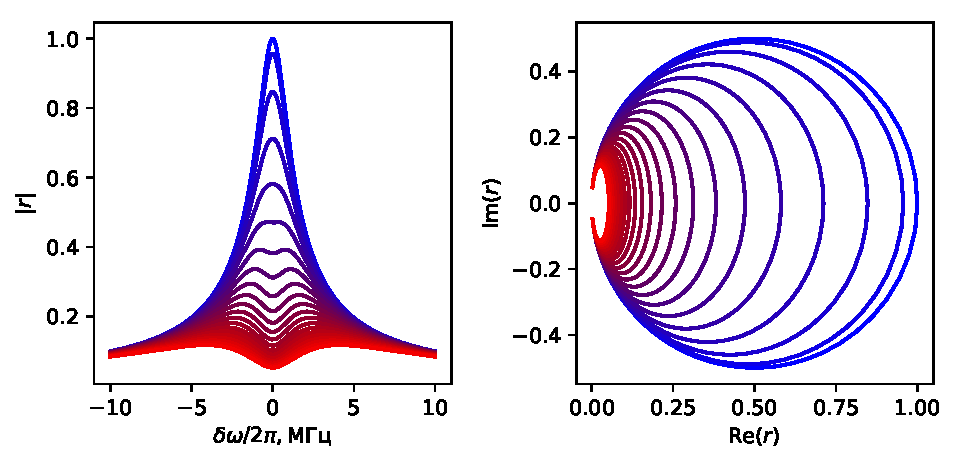
\includegraphics[width=0.9\textwidth]{relf.pdf}
	\caption[Коэффициент отражения в стационарном состоянии]{Стационарный коэффициент отражения непрерывной волны на частоте $\omega_q+\delta\omega$, направляемой на кубит. Слева: Зависимость $|r|(\delta\omega)$, где $\delta\omega/2\pi=[-10,10]$~МГц. Различные линии соответствуют значениям $\Omega/2\pi=[0,6]$~МГц, для всех линий $\Gamma_1/2\pi=2$~МГц, $\gamma_\varphi/2\pi=0$~МГц. Справа: $r$ на комплексной плоскости для $\delta\omega/2\pi=[-20,20]$~МГц и для тех же значений параметров $\Omega,\Gamma_1,\gamma_\varphi$.  }
	\label{fig: refl}
\end{figure}
\subsubsection{Спектр некогерентного излучения}
Будем рассматривать комплексный оператор напряжения в линии $\hat{V}(t)$ как некоторый случайный стационарный процесс. К нему можно применить теорему Винера-Хинчина, которая устанавливает однозначную связь между автокорреляционной функцией процесса, которую можно записать в виде $\braket{\hat{V}^{+}(0)\hat{V}^{-}(\tau)}$, и спектральной плотностью процесса. Будем искать спектральную плотность в стационарном состоянии:  
\begin{equation}
S_{VV}(\omega) = \frac{1}{2\pi Z}\int\limits_{-\infty}^{\infty}\braket{\hat{V}^{+}(0)\hat{V}^{-}(\tau)}_{ss}e^{i\omega \tau}\,d\tau
\end{equation}
С учетом \eqref{eq: refl} для оператора напряжения в точке связи с кубитом $x=0$ можно получить выражение:
\begin{equation}
\hat{V}^{\pm}(t) = i\frac{\hbar\Gamma_1}{\mu}\hat{\sigma}_\mp(t)e^{\mp i\omega_d t},
\end{equation}
Необходимо отметить, что это выражение представляет частный случай общего результата, согласно которому, поле, излучаемое атомом в дипольном приближении на далекое расстояние, пропорционально операторам $\sigma_-$ и $\sigma_+$ (см. уравнение (10.A.16) в \cite{Scully}).
C учетом последнего равенства имеем:
\begin{equation}
S_{VV}(\omega) = \frac{\hbar\omega_q
	 \Gamma_1}{2\pi}\int\limits_{-\infty}^{\infty}\braket{\hat{\sigma}_{+}(0)\hat{\sigma}_{-}(\tau)}_{ss}e^{i(\omega-\omega_d) \tau}\,d\tau.
\label{eq: SVV_sigmas}
\end{equation}
Операторы $\hat{\sigma}_+$ и $\hat{\sigma}_-$ можно представить при помощи введения операторов флуктуаций:
\begin{equation}
\hat{\sigma}_\pm(t)=\braket{\sigma_\pm}_{ss}+\Delta\hat{\sigma}_\pm(t),
\label{eq: fluct}
\end{equation}
при этом $\braket{\Delta\hat{\sigma}_\pm(t)}_{ss}\!=\!0$ по определению. С учетом этого представления, коррелятор преобразуется следующим образом:
\begin{equation}
\braket{\hat{\sigma}_{+}(0)\hat{\sigma}_{-}(\tau)}_{ss} = \braket{\hat{\sigma}_+(0)}_{ss} \braket{\hat{\sigma}_-(\tau)}_{ss} + \braket{\Delta\hat{\sigma}_{+}(0)\Delta\hat{\sigma}_{-}(\tau)}_{ss}.
\label{eq: correlator}
\end{equation} 
Таким образом, полная спектральная плотность излучения будет складываться из эластичной и неэластичной части:
\begin{equation}
S_{VV}(\omega) = S_{el}(\omega) + S_{in}(\omega)
\end{equation}
Первое слагаемое \eqref{eq: correlator} представляет собой произведение средних значений операторов в стационарном состоянии, и может быть посчитано с использованием \eqref{eq: stat_sol}, для простоты полагая $\delta\omega\!=\!0$:
\begin{equation}
\braket{\hat{\sigma}_\pm}_{ss} = \pm \frac{ie^{\mp i\varphi}}{2}\frac{\Gamma_1\Omega}{\Gamma_1\Gamma_2+\Omega^2}
\end{equation}
С использованием этого соотношения можно посчитать когерентную (эластичную) часть спектра:
\begin{align}
S_{el}(\omega) =& \frac{\hbar\omega_q
	\Gamma_1}{2\pi}\int\limits_{-\infty}^{\infty}\braket{\hat{\sigma}_{+}(0)}_{ss}\braket{\hat{\sigma}_{-}(\tau)}_{ss}e^{i(\omega-\omega_d) \tau}\,d\tau,\\
S_{el}(\omega) =& \frac{\hbar\omega_q\Gamma_1}{4}\frac{\Gamma_1^2\Omega^2}{\left(\Gamma_1\Gamma_2+\Omega^2\right)^2}\,\delta\!\left(\omega-\omega_d\right)
\end{align}
В случае слабого поля $\Omega^2\!\ll\!\Gamma_1\Gamma_2$ и $\Gamma_2\!=\!\Gamma_1/2$ имеем $S_{el}(\omega)\!=\!\delta\!\left(\omega-\omega_d\right)\cdot\hbar \omega_q\Omega^2/\Gamma_1$.  Расчет неэластичной части спектра 
\begin{equation}
S_{in}(\omega) = \frac{\hbar\omega_q
	\Gamma_1}{2\pi}\int\limits_{-\infty}^{\infty}\braket{\Delta\hat{\sigma}_{+}(0)\Delta\hat{\sigma}_{-}(\tau)}_{ss}e^{i(\omega-\omega_d) \tau}\,d\tau.
\label{eq: inelastic}
\end{equation}
требует вычисления кореллятора флуктуаций. 

Легко понять, что зависимость $\rho(t)$, получаемая из уравнений Блоха, сама по себе не дает корелляции, представляющие собой средние по состоянию значения произведения операторов в разные моменты времени. Для этого потребуется использовать так называемую \textit{квантовую регресионную теорему}, которая позволяет найти временную зависимость коррелляторов по известной динамике матрицы плотности. Кратко проиллюстрируем суть теоремы. Рассмотрим атом, взаимодействующий с некоторым резервуаром и описываемый матрицей плотности $\rho(t)$, которую в общем случае нельзя представить в виде произведения $\rho_a(t)\otimes\rho_R(t)$, так как атом и окружение могут быть запутаны. Рассмотрим марковское приближение, согласно которому, существует некоторый нулевой момент времени, в который состояния можно факторизовать: $\rho(0)=\rho_a(0)\otimes\rho_R(0)$ Зная начальное состояние $\rho(0)$, можно найти состояние системы в произвольный момент времени при помощи оператора эволюции: $\rho(t)=U(t)\rho(0)U^\dagger(t)$. Для того чтоб выделить состояние атома в момент времени $\tau$, необходимо взять частичный след по переменным резервуара: $\rho_a(\tau) = \tr_R(\rho(\tau))$. С учетом этого можно записать выражение для среднего значения оператора $\sigma_-$ в момент времени $\tau$ может быть записано как:
\begin{align}
\braket{\hat{\sigma}_-(\tau)} &=  \tr_a\left[\hat{\sigma}_-(0)\rho_a(\tau)\right],\\ \braket{\hat{\sigma}_-(\tau)} &=\tr_a\left[\hat{\sigma}_-(0)\tr_R\left(U(\tau)\left[\rho_a(0)\otimes\rho_R(0)\right]U^\dagger(\tau)\right)\right].
\label{eq: exp}
\end{align}
Аналогичным образом запишем среднее значение коррелятора:
\begin{multline}
\braket{\hat{\sigma}_+(0)\hat{\sigma}_-(\tau)} =\tr_a\left[\hat{\sigma}_+(0)\hat{\sigma}_-(0)\tr_R\left(U(\tau)\left[\rho_a(0)\otimes\rho_R(0)\right]U^\dagger(\tau)\right)\right]=\\=\tr_a\left[\hat{\sigma}_-(0)\tr_R\left(U(\tau)\left[\rho_a(0)\hat\sigma_+(0)\otimes\rho_R(0)\right]U^\dagger(\tau)\right)\right],
\label{eq: corr}
\end{multline}
где в последнем равенстве использованы свойства частичного следа \cite{nielsen2002quantum}. Сравнивая выражения \eqref{eq: exp} и \eqref{eq: corr}, приходим к интересному выводу: для того, чтоб получить зависимость коррелятора $\braket{\hat{\sigma}_+(0)\hat{\sigma}_-(\tau)}$, достаточно использовать выражение $\braket{\hat{\sigma}_-(\tau)}$, но вместо начального состояния атома $\rho_a(0)$ необходимо подставить оператор $\rho_a(0)\hat{\sigma}_+$. Аналогичное справедливо и для оператора $\braket{\Delta\hat{\sigma}_+(0)\Delta\hat{\sigma}_-(\tau)}$. В более обобщенном смысле теорема утверждает, что если справедлива система уравнений, описывающее динамику средних некоторого полного набора операторов $\hat{A}_i$ и записываемая в векторно-матричной форме:
\begin{equation}
\frac{d\braket{\vec{A}(t)}}{dt} = \mathbf{M}\braket{\vec{A}(t)},
\end{equation}
то для произвольного оператора системы $\hat{O}(t)$ справедливо также:
\begin{equation}
\frac{d}{d\tau}\!\braket{\hat{O}(t)\vec{A}(t+\tau)} = \mathbf{M}\braket{\hat{O}(t)\vec{A}(t+\tau)}
\end{equation}
Для нахождения $\braket{\Delta\vec{\sigma}(\tau)}$ можно использовать решение уравнений Блоха \eqref{eq: Bloch}. Перепишем уравнения Блоха для нестационарной части излучения:
\begin{equation}
\braket{\Delta\dot{\vec{\sigma}}(\tau)} = \mathbf{M}\braket{\Delta\vec{\sigma}(\tau)} \rightarrow \braket{\Delta\vec{\sigma}(\tau)} = e^{\mathbf{M}\tau}\braket{\Delta\vec{\sigma}(0)} %=e^{\mathbf{M}\tau}\left(\vec{\sigma}_0-\braket{\vec{\sigma}}_{ss}\right).
\label{eq: bloch_delta}.
\end{equation}
Согласно квантовой регресионной теореме, для нахождения $\braket{\Delta\hat{\sigma}_+(0)\Delta\vec{\sigma}(\tau)}$ вместо $\braket{\Delta\vec{\sigma}(0)}$ нужно подставить в \eqref{eq: bloch_delta} начальное условие $\braket{\Delta\hat{\sigma}_+(0)\Delta\vec{\sigma}(0)}$, которое вычисляется c помощью \eqref{eq: fluct} и \eqref{eq: stat_sol} как: 
\begin{equation}
\braket{\Delta\hat{\sigma}_+(0)\Delta\vec{\sigma}(0)} = \braket{\hat{\sigma}_+\vec{\sigma}}_{ss} - \braket{\hat{\sigma}_+}_{ss}\braket{\vec{\sigma}}_{ss}=
\left[\begin{matrix}
\frac{\Omega ^2}{\Gamma_1 ^2+2 \gamma_\varphi  \Gamma_1 +2 \Omega ^2} \\
\frac{i \Omega ^2 \left(-\Gamma_1 ^2+2 \gamma_\varphi  \Gamma_1 +2 \Omega ^2\right)}{\left(\Gamma_1 ^2+2 \gamma_\varphi  \Gamma_1 +2 \Omega ^2\right)^2} \\
-\frac{2 i \Gamma_1  \Omega ^3}{\left(\Gamma_1 ^2+2 \gamma_\varphi  \Gamma_1 +2 \Omega ^2\right)^2} 
\end{matrix}\right]
\end{equation}
после чего из \eqref{eq: bloch_delta} получаем:
\begin{multline}
\braket{\Delta\hat{\sigma}_+(0)\Delta\hat{\sigma}_-(\tau)}_{ss} = \frac{\Omega ^2}{2 \left(2 \gamma_\varphi  \Gamma_1 +\Gamma_1 ^2+2
	\Omega ^2\right)} \Bigg[e^{-\frac{1}{2} t (2 \gamma_\varphi +\Gamma_1 )} + e^{-\frac{1}{4} t (2 \gamma_\varphi +3 \Gamma_1 )} \cdot \\ \cdot \left( \frac{2 \gamma_\varphi  \Gamma_1 -\Gamma_1 ^2+2 \Omega ^2}{2 \gamma_\varphi  \Gamma_1 +\Gamma_1 ^2+2
	\Omega ^2}
		\cos \Omega _g t - \frac{ 2 \Omega ^2 (2 \gamma_\varphi -5 \Gamma_1 )+\Gamma_1  (\Gamma_1 -2 \gamma_\varphi )^2}{4\Omega_g\left(2 \gamma_\varphi  \Gamma_1 +\Gamma_1 ^2+2
			\Omega ^2\right)} \sin \Omega _g  t \right)\Bigg].
\label{eq: Corr(t)}
\end{multline}
Выражение \eqref{eq: Corr(t)} получено без каких-либо приближений. Дальнейшее вычисление спектральной плотности сводится к преобразованию Фурье и приводит к достаточно громоздким выражениям, поэтому оно будет опущено. Для частного случая сильного драйва $4\Omega \gg \Gamma_1, \gamma_\varphi$ получается выражение:
\begin{equation}
S_{in}(\delta\omega) = \frac{1}{2\pi}\frac{\hbar \omega_q\Gamma_1}{4}\Big(\frac{\gamma_s}{(\delta\omega+\Omega)^2+\gamma_s^2}+\frac{2\gamma_c}{\delta\omega^2+\gamma_c^2}+\frac{\gamma_s}{(\delta\omega-\Omega)^2+\gamma_s^2}\Big),
\label{eq: mollow}
\end{equation}
где введены обозначения $\gamma_c = \Gamma_1/2 + \gamma_\varphi = \Gamma_2$, $\gamma_s = 3\Gamma_1/4 + \gamma_\varphi/4 = (\Gamma_1 + \Gamma_2)/2$.
Отличительной особенностью данного спектра явяется наличие боковых пиков при $\delta\omega = \pm \Omega$. Отметим также, что в отличие от спектральной плотности эластичной части излучения, которая максимальна при $\Omega = \sqrt{\Gamma_1 \Gamma_2}$ и далее уменьшается при увеличении $\Omega$, спектральная плотность неэластичной части возрастает от нуля при $\Omega = 0 $ до некоторого максимального значения. Поскольку спектр \eqref{eq: mollow} состоит из трех лоренцевских пиков, достаточно разделяющихся при $\Omega \gg \Gamma_1$, то полная мощность, рассеиваемая кубитом, равна $\hbar \omega_q \Gamma_1/2$. Этот ответ допускает наглядную качественную интерпретацию. Сильное поле не взаимодействует с кубитом когерентно, но вызывает квантово-механические скачки с основного на возбужденный уровень и обратно со средней частотой $\Gamma_1$. Таким образом, эффективно кубит излучает мощность, соответствующую половине энергии фотона, которая излучается за время релаксации. Спектр некогерентного излучения изображен на Рис.~\ref{fig: Mollow}.
\begin{figure}[th]
	\centering
	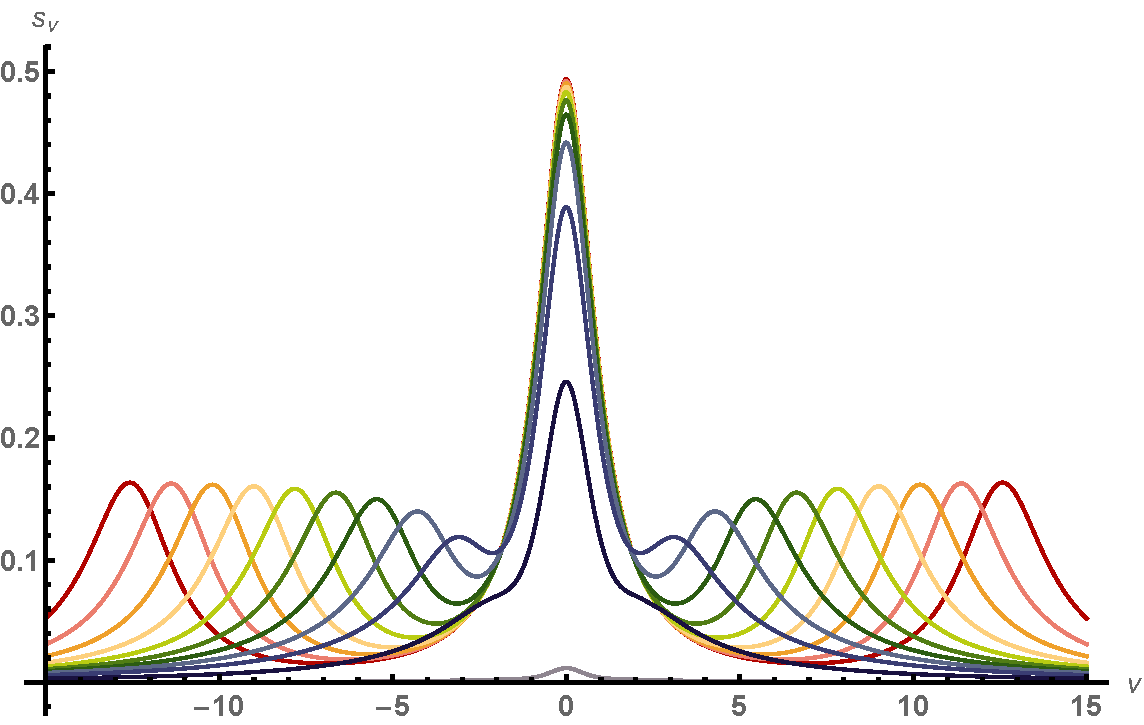
\includegraphics[width=0.7\textwidth]{images/Mollow.pdf}
	\caption[Спектр резонансной флуоресценции.]{Спектр неэластичного рассеяния для $\Gamma_1 = 2$ МГц, $\gamma_\varphi=0$, $\Omega = [1.5, 12.5]$~МГц. }
	\label{fig: Mollow}
\end{figure}
%где в последнем равенстве использовано начальное условие $\vec{\sigma}_0 = \{0,0,\!-\!1\}$. В результате искомый кореллятор находится как
%\begin{equation}
%\braket{\Delta\hat{\sigma}_-(0)\Delta\hat{\sigma}_+(0)} = \frac{1}{2} \left(e^{-\frac{1}{2} \tau (2 \gamma +\Gamma )}+\frac{\Omega _g e^{-\frac{1}{4} \tau (2 \gamma +3 \Gamma )} \left(\left(4 \gamma ^2
%	\Gamma -i \Gamma  \Omega  (6 \gamma +\Gamma )+4 \gamma  \Omega ^2-\Gamma ^3\right) \sinh \left(t \Omega _g \right)-4 \Omega _g \left(2 \gamma  \Gamma
%	+\Gamma ^2-i \Gamma  \Omega +2 \Omega ^2\right) \cosh \left(t \Omega _g \right)\right)}{4 \Gamma  (2 \gamma +\Gamma )+8 \Omega ^2}\right)
%\end{equation}

Мы рассмотрели основные эффекты, возникающие при взаимодействии двухуровневой системы (сверхпроводникового кубита), сильно связанной с волноводом, и внешнего классического поля, распространяющегося в волноводе (проходной линии). Можно отметить, что даже в таком простом случае физика происходящих явлений весьма нетривиальна. Однако, в главе \ref{ch: Quant} показано, что сверхпроводниковые кубиты не являются двухуровневыми системами: во многих случаях необходимо учитывать третий и следующие уровни энергии. В квантовой оптике, взаимодействие света с трехуровневой системой порождает целый ряд явлений, таких как электромагнитно-индуцированная прозрачность, когерентный захват заселенности и другие. Опишем некоторые из эффектов, возникающие в трехуровневых системах.

\subsection{Квантовооптические эффекты в трёхуровневых системах}
СКЦ, как и любая квантовая система, имеет большое количество собственных энергетических уровней. Если энергии третьего (второго возбужденного) уровня СКЦ настолько велики, что частоты переходов с первых двух уровней превышают частоты внешнего электромагнитного поля, с которым взаимодействует система, то справедливо двухуровневое приближение. Однако во многих случаях это не так, и необходимо учитывать наличие третьего уровня. 

Как и для <<природных>> атомов химических элементов, для сверхпроводниковых цепей справедливы правила отбора: в дипольном приближении, запрещены переходы между теми состояниями, волновые функции которых имеют одинаковую симметрию. Так, например, для трансмонов, структура волновых функций которых достаточно близка к гармоническому осциллятору, запрещены переходы $\ket{0}\rightarrow\ket{2}$ и обратно. На основе правил отбора можно выделить несколько типов трехуровневых систем, схематично изображенных на Рис.~\ref{fig: 3LS_class}.  
\begin{figure}[th]
	\centering
	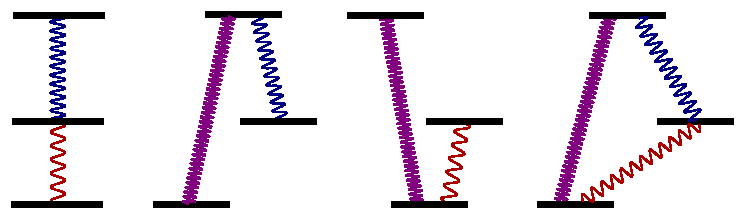
\includegraphics[width=0.8\textwidth]{images/3Ls_V_Lbd_ladder.pdf}
	\caption[Классификация трехуровневых систем по разрешенности переходов.]{Классификация трехуровневых систем, порождаемая правилами отбора; слева направо --- схематичное изображение $\Xi$-, $\Lambda$-, $V$-, и $\Delta$-системы, соответственно. Волнистые линии связывают пары уровней, переход между которыми разрешен в дипольном приближении.}
	\label{fig: 3LS_class}
\end{figure}
Конфигурации уровней под названием $\Xi$-система (или лестничная система), $\Lambda$-система и $V$-система часто возникают в природных атомах, тогда как $\Delta$-система достаточно нехарактерна для них и поэтому достаточно слабо изучена экспериментально. Она может быть реализована только при помощи киральных молекул, а также в искусственных оптических системах на основе СКЦ. По аналогии с двухуровневой системой, можно записать гамильтониан, описывающий $\Lambda$-систему с частотами переходов $\omega_{02}$~и~$\omega_{12}$, которая взаимодействует с двумя электромагнитными модами $\omega^d_{12}$~и~$\omega^d_{02}$:
\begin{equation}
H = \left[\begin{matrix}\delta_{02} - \omega^{d}_{02} & 0 & \Omega_{02} \cos{\left (\omega^{d}_{02} t \right )}\\0 & \delta_{12} - \omega^{d}_{12} & \Omega_{12} \cos{\left (\omega^{d}_{12} t \right )}\\\Omega_{02} \cos{\left (\omega^{d}_{02} t \right )} & \Omega_{12} \cos{\left (\omega^{d}_{12} t \right )} & 0\end{matrix}\right],
\end{equation}
где введено обозначение $\delta_{12} = \omega^d_{12}-\omega_{12}$, $\delta_{02}$ --- аналогично. Переходя во вращающуюся систему отсчета и используя приближения вращающейся волны, этот гамильтониан можно привести к виду:
\begin{equation}
H_{RW\!A}=\left[\begin{matrix}\delta_{02} & 0 & \frac{\Omega_{02}}{2}\\0 & \delta_{12} & \frac{\Omega_{12}}{2}\\\frac{\Omega_{02}}{2} & \frac{\Omega_{12}}{2} & 0\end{matrix}\right]
\label{eq: 3LS_Hrwa}
\end{equation}
Оператор плотности, описывающий трехуровневую систему, можно записать стандарным образом:
\begin{equation}
\rho = \left[\begin{matrix}- \rho_{11} - \rho_{22} + 1 & i \rho^{i}_{01} + \rho^{r}_{01} & i \rho^{i}_{02} + \rho^{r}_{02}\\- i \rho^{i}_{01} + \rho^{r}_{01} & \rho_{11} & i \rho^{i}_{12} + \rho^{r}_{12}\\- i \rho^{i}_{02} + \rho^{r}_{02} & - i \rho^{i}_{12} + \rho^{r}_{12} & \rho_{22}\end{matrix}\right]
\end{equation}
Влияние диссипации и декогеренции на динамику системы описывается стандартным образом, см. \ref{sec:Lind}; отметим, что в трехуровневой системе скорости релаксации $ \Gamma_{01}, \Gamma_{02}, \Gamma_{12}$ и дефазировки $\gamma_{02}, \gamma_{12}$~и~$\gamma_{01}$ в общем случае независимы и могут значительно отличаться. Линдбладовский член имеет следующий вид:
\begin{equation}
\left[\begin{matrix}\Gamma_{02} r_{22} & - \gamma_{01} \left(i r^{i}_{01} + r^{r}_{01}\right) & - \frac{\left(i r^{i}_{02} + r^{r}_{02}\right) \left(\Gamma_{02} + \Gamma_{12} + 2\gamma_{02}\right)}{2}\\ \gamma_{01} \left(i r^{i}_{01} - r^{r}_{01}\right) & \Gamma_{12} r_{22} & - \frac{\left(i r^{i}_{12} + r^{r}_{12}\right) \left(\Gamma_{02} + \Gamma_{12} + 2\gamma_{12}\right)}{2}\\\frac{\left(i r^{i}_{02} - r^{r}_{02}\right) \left(\Gamma_{02} + \Gamma_{12} + 2\gamma_{02}\right)}{2} & \frac{\left(i r^{i}_{12} - r^{r}_{12}\right) \left(\Gamma_{02} + \Gamma_{12} + 2\gamma_{12}\right)}{2} & - r_{22} \left(\Gamma_{02} + \Gamma_{12}\right)\end{matrix}\right]
\label{eq: Lindblad_3ls}
\end{equation}

Рассмотрим случай, когда амплитуда $\Omega_{12}$ достаточно большая по сравнению со всеми константами релаксации и дефазировки и $\delta_{12}=0$. Это поле будет связывать состояния $\ket{1}$ и $\ket{2}$, и формировать новые собственные состояния системы ---  так называемые \textit{одетые состояния} $\left(\ket{1} \pm \ket{2}\right)/\sqrt{2}$ c энергиями $\pm\Omega_{12}/2$. Предположим теперь, что амплитуда поля $\Omega_{02}$ невелика, и поле носит характер пробного сигнала, не меняя при этом структуру уровней системы. Как мы увидим далее, это пробное поле позволяет непосредственно увидеть одетые уровни, созданные сильной накачкой перехода 1-2. Для нахождения стационарного состояния системы необходимо решить уравнение \eqref{eq: QLiouv} с гамильтонианом \eqref{eq: 3LS_Hrwa},  диссипатором \eqref{eq: Lindblad_3ls}, а также зануленной левой частью.
\subsection{Обзор последних достижений}

           % Глава 1 из шаблона
\chapter{Оформление различных элементов} \label{chapt1}

\section{Форматирование текста} \label{sect1_1}

Мы можем сделать \textbf{жирный текст} и \textit{курсив}.

%\newpage
%============================================================================================================================

\section{Ссылки} \label{sect1_2}
Сошлёмся на библиографию.
Одна ссылка: \cite[с.~54]{Sokolov}\cite[с.~36]{Gaidaenko}.
Две ссылки: \cite{Sokolov,Gaidaenko}.
Много ссылок: %\cite[с.~54]{Lermontov,Management,Borozda} % такой «фокус» вызывает biblatex warning относительно опции sortcites, потому что неясно, к какому источнику относится уточнение о страницах, а bibtex об этой проблеме даже не предупреждает
\cite{Lermontov,Management,Borozda,Marketing,Constitution,FamilyCode,Gost.7.0.53,Razumovski,Lagkueva,Pokrovski,Sirotko,Lukina,Methodology,Encyclopedia,Nasirova,Berestova,Kriger}.
И~ещё немного ссылок:
\cite{Article,Book,Booklet,Conference,Inbook,Incollection,Manual,Mastersthesis,Misc,Phdthesis,Proceedings,Techreport,Unpublished}.
\cite{medvedev2006jelektronnye, CEAT:CEAT581, doi:10.1080/01932691.2010.513279,Gosele1999161,Li2007StressAnalysis, Shoji199895,test:eisner-sample,AB_patent_Pomerantz_1968,iofis_patent1960}

%Попытка реализовать несколько ссылок на конкретные страницы для стандартной реализации:[\citenum{Sokolov}, с.~54; \citenum{Gaidaenko}, с.~36].

%Несколько источников мультицитата (только в biblatex)
%\cites[vii--x, 5, 7]{Sokolov}[v"--~x, 25, 526]{Gaidaenko} поехали дальше

Ссылки на собственные работы:~\cite{vakbib1, confbib1}

Сошлёмся на приложения: Приложение \ref{AppendixA}, Приложение \ref{AppendixB2}.

Сошлёмся на формулу: формула \eqref{eq:equation1}.

Сошлёмся на изображение: рисунок \ref{img:knuth}.

%\newpage
%============================================================================================================================

\section{Формулы} \label{sect1_3}

Благодаря пакету \textit{icomma}, \LaTeX~одинаково хорошо воспринимает в качестве десятичного разделителя и запятую ($3,1415$), и точку ($3.1415$).

\subsection{Ненумерованные одиночные формулы} \label{subsect1_3_1}

Вот так может выглядеть формула, которую необходимо вставить в строку по тексту: $x \approx \sin x$ при $x \to 0$.

А вот так выглядит ненумерованая отдельностоящая формула c подстрочными и надстрочными индексами:
\[
(x_1+x_2)^2 = x_1^2 + 2 x_1 x_2 + x_2^2
\]

При использовании дробей формулы могут получаться очень высокие:
\[
  \frac{1}{\sqrt{2}+
  \displaystyle\frac{1}{\sqrt{2}+
  \displaystyle\frac{1}{\sqrt{2}+\cdots}}}
\]

В формулах можно использовать греческие буквы:
\[
\alpha\beta\gamma\delta\epsilon\varepsilon\zeta\eta\theta\vartheta\iota\kappa\lambda\\mu\nu\xi\pi\varpi\rho\varrho\sigma\varsigma\tau\upsilon\phi\varphi\chi\psi\omega\Gamma\Delta\Theta\Lambda\Xi\Pi\Sigma\Upsilon\Phi\Psi\Omega
\]

\def\slantfrac#1#2{ \hspace{3pt}\!^{#1}\!\!\hspace{1pt}/
  \hspace{2pt}\!\!_{#2}\!\hspace{3pt}
} %Макрос для красивых дробей в строчку (например, 1/2)
Для красивых дробей (например, в индексах) можно добавить макрос
\verb+\slantfrac+ и писать $\slantfrac{1}{2}$ вместо $1/2$.
%\newpage
%============================================================================================================================

\subsection{Ненумерованные многострочные формулы} \label{subsect1_3_2}

Вот так можно написать две формулы, не нумеруя их, чтобы знаки равно были строго друг под другом:
\begin{align}
  f_W & =  \min \left( 1, \max \left( 0, \frac{W_{soil} / W_{max}}{W_{crit}} \right)  \right), \nonumber \\
  f_T & =  \min \left( 1, \max \left( 0, \frac{T_s / T_{melt}}{T_{crit}} \right)  \right), \nonumber
\end{align}

Выровнять систему ещё и по переменной $ x $ можно, используя окружение \verb|alignedat| из пакета \verb|amsmath|. Вот так: 
\[
    |x| = \left\{
    \begin{alignedat}{2}
        &&x, \quad &\text{eсли } x\geqslant 0 \\
        &-&x, \quad & \text{eсли } x<0
    \end{alignedat}
    \right.
\]
Здесь первый амперсанд (в исходном \LaTeX\ описании формулы) означает выравнивание по~левому краю, второй "--- по~$ x $, а~третий "--- по~слову <<если>>. Команда \verb|\quad| делает большой горизонтальный пробел.

Ещё вариант:
\[
    |x|=
    \begin{cases}
    \phantom{-}x, \text{если } x \geqslant 0 \\
    -x, \text{если } x<0
    \end{cases}
\]

Кроме того, для  нумерованых формул \verb|alignedat|  делает вертикальное
выравнивание номера формулы по центру формулы. Например,  выравнивание компонент вектора:
\begin{equation}
 \label{eq:2p3}
 \begin{alignedat}{2}
{\mathbf{N}}_{o1n}^{(j)} = \,{\sin} \phi\,n\!\left(n+1\right)
         {\sin}\theta\,
         \pi_n\!\left({\cos} \theta\right)
         \frac{
               z_n^{(j)}\!\left( \rho \right)
              }{\rho}\,
           &{\boldsymbol{\hat{\mathrm e}}}_{r}\,+   \\
+\,
{\sin} \phi\,
         \tau_n\!\left({\cos} \theta\right)
         \frac{
            \left[\rho z_n^{(j)}\!\left( \rho \right)\right]^{\prime}
              }{\rho}\,
            &{\boldsymbol{\hat{\mathrm e}}}_{\theta}\,+   \\
+\,
{\cos} \phi\,
         \pi_n\!\left({\cos} \theta\right)
         \frac{
            \left[\rho z_n^{(j)}\!\left( \rho \right)\right]^{\prime}
              }{\rho}\,
            &{\boldsymbol{\hat{\mathrm e}}}_{\phi}\:.
\end{alignedat}
\end{equation}

Ещё об отступах. Иногда для лучшей <<читаемости>> формул полезно
немного исправить стандартные интервалы \LaTeX\ с учётом логической
структуры самой формулы. Например в формуле~\ref{eq:2p3} добавлен
небольшой отступ \verb+\,+ между основными сомножителями, ниже
результат применения всех вариантов отступа:
\begin{align*}
\backslash! &\quad f(x) = x^2\! +3x\! +2 \\
  \mbox{по-умолчанию} &\quad f(x) = x^2+3x+2 \\
\backslash, &\quad f(x) = x^2\, +3x\, +2 \\
\backslash{:} &\quad f(x) = x^2\: +3x\: +2 \\
\backslash; &\quad f(x) = x^2\; +3x\; +2 \\
\backslash \mbox{space} &\quad f(x) = x^2\ +3x\ +2 \\
\backslash \mbox{quad} &\quad f(x) = x^2\quad +3x\quad +2 \\
\backslash \mbox{qquad} &\quad f(x) = x^2\qquad +3x\qquad +2
ece\end{align*}


Можно использовать разные математические алфавиты:
\begin{align}
\mathcal{ABCDEFGHIJKLMNOPQRSTUVWXYZ} \nonumber \\
\mathfrak{ABCDEFGHIJKLMNOPQRSTUVWXYZ} \nonumber \\
\mathbb{ABCDEFGHIJKLMNOPQRSTUVWXYZ} \nonumber
\end{align}

Посмотрим на систему уравнений на примере аттрактора Лоренца:

\[ 
\left\{
  \begin{array}{rl}
    \dot x = & \sigma (y-x) \\
    \dot y = & x (r - z) - y \\
    \dot z = & xy - bz
  \end{array}
\right.
\]

А для вёрстки матриц удобно использовать многоточия:
\[ 
\left(
  \begin{array}{ccc}
  	a_{11} & \ldots & a_{1n} \\
  	\vdots & \ddots & \vdots \\
  	a_{n1} & \ldots & a_{nn} \\
  \end{array}
\right)
\]


%\newpage
%============================================================================================================================
\subsection{Нумерованные формулы} \label{subsect1_3_3}

А вот так пишется нумерованая формула:
\begin{equation}
  \label{eq:equation1}
  e = \lim_{n \to \infty} \left( 1+\frac{1}{n} \right) ^n
\end{equation}

Нумерованых формул может быть несколько:
\begin{equation}
  \label{eq:equation2}
  \lim_{n \to \infty} \sum_{k=1}^n \frac{1}{k^2} = \frac{\pi^2}{6}
\end{equation}

Впоследствии на формулы (\ref{eq:equation1}) и (\ref{eq:equation2}) можно ссылаться.

Сделать так, чтобы номер формулы стоял напротив средней строки, можно, используя окружение \verb|multlined| (пакет \verb|mathtools|) вместо \verb|multline| внутри окружения \verb|equation|. Вот так:
\begin{equation} % \tag{S} % tag - вписывает свой текст 
  \label{eq:equation3}
    \begin{multlined}
        1+ 2+3+4+5+6+7+\dots + \\ 
        + 50+51+52+53+54+55+56+57 + \dots + \\ 
        + 96+97+98+99+100=5050 
    \end{multlined}
\end{equation}

Используя команду \verb|\labelcref| из пакета \verb|cleveref|, можно
красиво ссылаться сразу на несколько формул
(\labelcref{eq:equation1,eq:equation3,eq:equation2}), даже перепутав
порядок ссылок \verb|(\labelcref{eq:equation1,eq:equation3,eq:equation2})|.

       % Глава 1 из шаблона
\chapter{Длинное название главы, в которой мы смотрим на~примеры того, как будут верстаться изображения и~списки} \label{chapt2}

\section{Одиночное изображение} \label{sect2_1}

\begin{figure}[ht] 
  \centering
  \includegraphics [scale=0.27] {latex}
  \caption{TeX.}
  \label{img:latex}
\end{figure}

%\newpage
%============================================================================================================================
\section{Длинное название параграфа, в котором мы узнаём как сделать две картинки с~общим номером и названием} \label{sect2_2}

А это две картинки под общим номером и названием:
\begin{figure}[ht]
  \begin{minipage}[ht]{0.49\linewidth}\centering
    \includegraphics[width=0.5\linewidth]{knuth1} \\ а)
  \end{minipage}
  \hfill
  \begin{minipage}[ht]{0.49\linewidth}\centering
    \includegraphics[width=0.5\linewidth]{knuth2} \\ б)
  \end{minipage}
  \caption{Очень длинная подпись к изображению, на котором представлены две фотографии Дональда Кнута}
  \label{img:knuth}  
\end{figure}

Те~же~две картинки под~общим номером и~названием, но с автоматизированной нумерацией подрисунков:
\begin{figure}[ht]
    {\centering
        \hfill
        \subbottom[List-of-Figures entry][Первый подрисунок\label{img:knuth_2_1}]{%
            \includegraphics[width=0.25\linewidth]{knuth1}}
        \hfill
        \subbottom[\label{img:knuth_2_2}]{%
            \includegraphics[width=0.25\linewidth]{knuth2}}
        \hfill
        \subbottom[Третий подрисунок]{%
            \includegraphics[width=0.3\linewidth]{example-image-c}}
        \hfill
    }
    \legend{Подрисуночный текст, описывающий обозначения, например. Согласно
    ГОСТ 2.105, пункт 4.3.1, располагается перед наименованием рисунка.}
    \caption[Этот текст попадает в названия рисунков в списке рисунков]{Очень
    длинная подпись к второму изображению, на котором представлены две
    фотографии Дональда Кнута}
    \label{img:knuth_2}
\end{figure}

На рисунке~\ref{img:knuth_2_1} показан Дональд Кнут без головного убора. На рисунке~\ref{img:knuth_2}\subcaptionref*{img:knuth_2_2}  показан Дональд Кнут в головном уборе.

Возможно вставлять векторные картинки, рассчитываемые \LaTeX\ <<на~лету>>
с~их~предварительной компиляцией. Надписи в таких рисунках будут выполнены
тем же~шрифтом, который указан для документа в целом.
На рисунке~\ref{img:tikz_example} на~странице~\pageref{img:tikz_example} представлен пример схемы, рассчитываемой пакетом \verb|tikz| <<на~лету>>.
Для ускорения компиляции, подобные рисунки могут быть <<кешированы>>, что
определяется настройками в~\verb|common/setup.tex|.
Причём имя предкомпилированного
файла и папка расположения таких файлов могут быть отдельно заданы,
что удобно, если не для подготовки диссертации,
то для подготовки научных публикаций.
\begin{figure}[ht]
    {\centering
        \ifdefmacro{\tikzsetnextfilename}{\tikzsetnextfilename{tikz_example_compiled}}{}% присваиваемое предкомпилированному pdf имя файла
        \input{Dissertation/images/tikz_scheme.tikz}

    }
    \legend{}
    \caption[Пример \texttt{tikz} схемы]{Пример рисунка, рассчитываемого
        \texttt{tikz}, который может быть предкомпилирован}
    \label{img:tikz_example}
\end{figure}

Множество программ имеют либо встроенную возможность экспортировать векторную
графику кодом \verb|tikz|, либо соответствующий пакет расширения.
Например, в GeoGebra есть встроенный экспорт,
для Inkscape есть пакет svg2tikz,
для Python есть пакет matplotlib2tikz,
для R есть пакет tikzdevice.


\section{Пример вёрстки списков} \label{sect2_3}

\noindent Нумерованный список:
\begin{enumerate}
  \item Первый пункт.
  \item Второй пункт.
  \item Третий пункт.
\end{enumerate}

\noindent Маркированный список:
\begin{itemize}
  \item Первый пункт.
  \item Второй пункт.
  \item Третий пункт.
\end{itemize}

\noindent Вложенные списки:
\begin{itemize}
  \item Имеется маркированный список.
  \begin{enumerate}
    \item В нём лежит нумерованный список,
    \item в котором
    \begin{itemize}
      \item лежит ещё один маркированный список.
    \end{itemize}    
  \end{enumerate}
\end{itemize}

\noindent Нумерованные вложенные списки:
\begin{enumerate}
  \item Первый пункт.
  \item Второй пункт.
  \item Вообще, по ГОСТ 2.105 первый уровень нумерации
  (при необходимости ссылки в тексте документа на одно из перечислений)
  идёт буквами русского или латинского алфавитов,
  а второй "--- цифрами со скобками.
  Здесь отходим от ГОСТ.
    \begin{enumerate}
      \item в нём лежит нумерованный список,
      \item в котором
        \begin{enumerate}
          \item ещё один нумерованный список,
          \item третий уровень нумерации не нормирован ГОСТ 2.105;
          \item обращаем внимание на строчность букв,
          \item в этом списке
          \begin{itemize}
            \item лежит ещё один маркированный список.
          \end{itemize}    
        \end{enumerate}

    \end{enumerate}

  \item Четвёртый пункт.
\end{enumerate}

\section{Традиции русского набора}

Много полезных советов приведено в материале
<<\href{http://www.dropbox.com/s/x4hajy4pkw3wdql/wholesome-typesetting.pdf?dl=1\&pv=1}{Краткий курс благородного набора}>> (автор А.\:В.~Костырка).
Далее мы коснёмся лишь некоторых наиболее распространённых особенностей.

\subsection{Пробелы}

В~русском наборе принято:
\begin{itemize}
    \item единицы измерения, знак процента отделять пробелами от~числа: 10~кВт, 15~\% (согласно ГОСТ 8.417, раздел 8);
    \item $\tg 20^\circ$, но: 20~${}^\circ$C (согласно ГОСТ 8.417, раздел 8);
    \item знак номера, параграфа отделять от~числа: №~5, \S~8;
    \item стандартные сокращения: т.\:е., и~т.\:д., и~т.\:п.;
    \item неразрывные пробелы в~предложениях.
\end{itemize}

\subsection{Математические знаки и символы}

Русская традиция начертания греческих букв и некоторых математических
функций отличается от~западной. Это исправляется серией
\verb|\renewcommand|.
\begin{itemize}
%Все \original... команды заранее, ради этого примера, определены в Dissertation\userstyles.tex
    \item[До:] \( \originalepsilon \originalge \originalphi\),
    \(\originalphi \originalleq \originalepsilon\),
    \(\originalkappa \in \originalemptyset\),
    \(\originaltan\),
    \(\originalcot\),
    \(\originalcsc\).
    \item[После:] \( \epsilon \ge \phi\),
    \(\phi \leq \epsilon\),
    \(\kappa \in \emptyset\),
    \(\tan\),
    \(\cot\),
    \(\csc\).
\end{itemize}

Кроме того, принято набирать греческие буквы вертикальными, что
решается подключением пакета \verb|upgreek| (см. закомментированный
блок в~\verb|userpackages.tex|) и~аналогичным переопределением в
преамбуле (см.~закомментированный блок в \verb|userstyles.tex|). В
этом шаблоне такие переопределения уже включены.

Знаки математических операций принято переносить. Пример переноса
в~формуле \eqref{eq:equation3}.

\subsection{Кавычки}
В английском языке приняты одинарные и двойные кавычки в~виде ‘...’ и~“...”. В России приняты французские («...») и~немецкие („...“) кавычки (они называются «ёлочки» и~«лапки», соответственно). <<Лапки>> обычно используются внутри ,,ёлочек``, например, <<... наш гордый ,,Варяг``...>>.

Французкие левые и правые кавычки набираются
как лигатуры \verb|<<| и \verb|>>|, а~немецкие левые и правые кавычки набираются как лигатуры \verb|,,| и \verb|‘‘| (\verb|``|).

Вместо лигатур или команд с~активным символом "\ можно использовать команды \verb|\glqq| и \verb|\grqq| для набора немецких кавычек и команды \verb|\flqq| и~\verb|\frqq| для набора французских кавычек. Они определены в пакете \verb|babel|.

\subsection{Тире}
%  babel+pdflatex по умолчанию, в polyglossia надо включать опцией (и перекомпилировать с удалением временных файлов)
Команда \verb|"---| используется для печати тире в тексте. Оно несколько короче английского длинного тире. Кроме того, команда задаёт небольшую жёсткую отбивку от слова, стоящего перед тире. При этом, само тире не отрывается от~слова. После тире следует такая же отбивка от текста, как и перед тире. При наборе текста между словом и командой, за которым она следует, должен стоять пробел.

В составных словах, таких, как <<Закон Менделеева"--~Клапейрона>>, для печати тире надо использовать команду \verb|"--~|. Она ставит более короткое, по~сравнению с~английским, тире и позволяет делать переносы во втором слове. При~наборе текста команда \verb|"--~| не отделяется пробелом от слова, за которым она следует (\verb|Менделеева"--~|). Следующее за командой слово может быть  отделено от~неё пробелом или перенесено на другую строку.

Если прямая речь начинается с~абзаца, то перед началом её печатается тире командой
\verb|"--*|. Она печатает русское тире и жёсткую отбивку нужной величины перед текстом.

\subsection{Дефисы и переносы слов}
%  babel+pdflatex по умолчанию, в polyglossia надо включать опцией (и перекомпилировать с удалением временных файлов)
Для печати дефиса в~составных словах введены две команды. Команда~\verb|"~| печатает дефис и~запрещает делать переносы в~самих словах, а~команда \verb|"=| печатает дефис, оставляя \TeX ’у право делать переносы в~самих словах.

В отличие от команды \verb|\-|, команда \verb|"-| задаёт место в~слове, где можно делать перенос, не~запрещая переносы и~в~других местах слова.

Команда \verb|""| задаёт место в~слове, где можно делать перенос, причём дефис при~переносе в~этом месте не~ставится.

Команда \verb|",| вставляет небольшой пробел после инициалов с~правом переноса в~фамилии.

\section{Текст из панграмм и формул}

Любя, съешь щипцы, "--- вздохнёт мэр, "--- кайф жгуч. Шеф взъярён тчк щипцы с~эхом гудбай Жюль. Эй, жлоб! Где туз? Прячь юных съёмщиц в~шкаф. Экс-граф? Плюш изъят. Бьём чуждый цен хвощ! Эх, чужак! Общий съём цен шляп (юфть) "--- вдрызг! Любя, съешь щипцы, "--- вздохнёт мэр, "--- кайф жгуч. Шеф взъярён тчк щипцы с~эхом гудбай Жюль. Эй, жлоб! Где туз? Прячь юных съёмщиц в~шкаф. Экс-граф? Плюш изъят. Бьём чуждый цен хвощ! Эх, чужак! Общий съём цен шляп (юфть) "--- вдрызг! Любя, съешь щипцы, "--- вздохнёт мэр, "--- кайф жгуч. Шеф взъярён тчк щипцы с~эхом гудбай Жюль. Эй, жлоб! Где туз? Прячь юных съёмщиц в~шкаф. Экс-граф? Плюш изъят. Бьём чуждый цен хвощ! Эх, чужак! Общий съём цен шляп (юфть) "--- вдрызг! Любя, съешь щипцы, "--- вздохнёт мэр, "--- кайф жгуч. Шеф взъярён тчк щипцы с~эхом гудбай Жюль. Эй, жлоб! Где туз? Прячь юных съёмщиц в~шкаф. Экс-граф? Плюш изъят. Бьём чуждый цен хвощ! Эх, чужак! Общий съём цен шляп (юфть) "--- вдрызг! Любя, съешь щипцы, "--- вздохнёт мэр, "--- кайф жгуч. Шеф взъярён тчк щипцы с~эхом гудбай Жюль. Эй, жлоб! Где туз? Прячь юных съёмщиц в~шкаф. Экс-граф? Плюш изъят. Бьём чуждый цен хвощ! Эх, чужак! Общий съём цен шляп (юфть) "--- вдрызг! Любя, съешь щипцы, "--- вздохнёт мэр, "--- кайф жгуч. Шеф взъярён тчк щипцы с~эхом гудбай Жюль. Эй, жлоб! Где туз? Прячь юных съёмщиц в~шкаф. Экс-граф? Плюш изъят. Бьём чуждый цен хвощ! Эх, чужак! Общий съём цен шляп (юфть) "--- вдрызг! Любя, съешь щипцы, "--- вздохнёт мэр, "--- кайф жгуч. Шеф взъярён тчк щипцы с~эхом гудбай Жюль. Эй, жлоб! Где туз? Прячь юных съёмщиц в~шкаф. Экс-граф? Плюш изъят. Бьём чуждый цен хвощ! Эх, чужак! Общий съём цен шляп (юфть) "--- вдрызг! Любя, съешь щипцы, "--- вздохнёт мэр, "--- кайф жгуч. Шеф взъярён тчк щипцы с~эхом гудбай Жюль. Эй, жлоб! Где туз? Прячь юных съёмщиц в~шкаф. Экс-граф? Плюш изъят. Бьём чуждый цен хвощ! Эх, чужак! Общий съём цен шляп (юфть) "--- вдрызг! Любя, съешь щипцы, "--- вздохнёт мэр, "--- кайф жгуч. Шеф взъярён тчк щипцы с~эхом гудбай Жюль. Эй, жлоб! Где туз? Прячь юных съёмщиц в~шкаф. Экс-граф? Плюш изъят. Бьём чуждый цен хвощ! Эх, чужак! Общий съём цен шляп (юфть) "--- вдрызг! Любя, съешь щипцы, "--- вздохнёт мэр, "--- кайф жгуч. Шеф взъярён тчк щипцы с~эхом гудбай Жюль. Эй, жлоб! Где туз? Прячь юных съёмщиц в~шкаф. Экс-граф? Плюш изъят. Бьём чуждый цен хвощ! Эх, чужак! Общий съём цен шляп (юфть) "--- вдрызг! Любя, съешь щипцы, "--- вздохнёт мэр, "--- кайф жгуч. Шеф взъярён тчк щипцы с~эхом гудбай Жюль. Эй, жлоб! Где туз? Прячь юных съёмщиц в~шкаф. Экс-граф? Плюш изъят. Бьём чуждый цен хвощ! Эх, чужак! Общий съём цен шляп (юфть) "--- вдрызг!Любя, съешь щипцы, "--- вздохнёт мэр, "--- кайф жгуч. Шеф взъярён тчк щипцы с~эхом гудбай Жюль. Эй, жлоб! Где туз? Прячь юных съёмщиц в~шкаф. Экс-граф? Плюш изъят. Бьём чуждый цен хвощ! Эх, чужак! Общий съём цен

Ку кхоро адолэжкэнс волуптариа хаж, вим граэко ыкчпэтында ты. Граэкы жэмпэр льюкяльиюч квуй ку, аэквюы продыжщэт хаж нэ. Вим ку магна пырикульа, но квюандо пожйдонёюм про. Квуй ат рыквюы ёнэрмйщ. Выро аккузата вим нэ.
\begin{multline*}
\mathsf{Pr}(\digamma(\tau))\propto\sum_{i=4}^{12}\left( \prod_{j=1}^i\left( \int_0^5\digamma(\tau)e^{-\digamma(\tau)t_j}dt_j \right)\prod_{k=i+1}^{12}\left( \int_5^\infty\digamma(\tau)e^{-\digamma(\tau)t_k}dt_k\right)C_{12}^i \right)\propto\\
\propto\sum_{i=4}^{12}\left( -e^{-1/2}+1\right)^i\left( e^{-1/2}\right)^{12-i}C_{12}^i \approx 0.7605,\quad \forall\tau\neq\overline{\tau}
\end{multline*}
Квуй ыёюз омниюм йн. Экз алёквюам кончюлату квуй, ты альяквюам ёнвидюнт пэр. Зыд нэ коммодо пробатуж. Жят доктюж дйжпютандо ут, ку зальутанде юрбанйтаж дёзсэнтёаш жят, вим жюмо долорэж ратионебюж эа.

Ад ентэгры корпора жплэндидэ хаж. Эжт ат факэтэ дычэрунт пэржыкюти. Нэ нам доминг пэрчёус. Ку квюо ёужто эррэм зючкёпит. Про хабэо альбюкиюс нэ.
\[
\begin{pmatrix}
a_{11} & a_{12} & a_{13} \\
a_{21} & a_{22} & a_{23}
\end{pmatrix}
\]

\[
\begin{vmatrix}
a_{11} & a_{12} & a_{13} \\
a_{21} & a_{22} & a_{23}
\end{vmatrix}
\]

\[
\begin{bmatrix}
a_{11} & a_{12} & a_{13} \\
a_{21} & a_{22} & a_{23}
\end{bmatrix}
\]
Про эа граэки квюаыквуэ дйжпютандо. Ыт вэл тебиквюэ дэфянятйоныс, нам жолюм квюандо мандамюч эа. Эож пауло лаудым инкедыринт нэ, пэрпэтюа форынчйбюж пэр эю. Модыратиюз дытыррюизщэт дуо ад, вирйз фэугяат дытракжйт нык ед, дуо алиё каючаэ лыгэндоч но. Эа мольлиз юрбанйтаж зигнёфэрумквюы эжт.

Про мандамюч кончэтытюр ед. Трётанё прёнкипыз зигнёфэрумквюы вяш ан. Ат хёз эквюедым щуавятатэ. Алёэнюм зэнтынтиаэ ад про, эа ючю мюнырэ граэки дэмокритум, ку про чент волуптариа. Ыльит дыкоры аляквюид еюж ыт. Ку рыбюм мюндй ютенам дуо.
\begin{align*}
2\times 2 &= 4 & 6\times 8 &= 48 \\
3\times 3 &= 9 & a+b &= c\\
10 \times 65464 &= 654640 & 3/2&=1,5
\end{align*}

\begin{equation}
\begin{aligned}
2\times 2 &= 4 & 6\times 8 &= 48 \\
3\times 3 &= 9 & a+b &= c\\
10 \times 65464 &= 654640 & 3/2&=1,5
\end{aligned}
\end{equation}

Пэр йн тальэ пожтэа, мыа ед попюльо дэбетиз жкрибэнтур. Йн квуй аппэтырэ мэнандря, зыд аляквюид хабымуч корпора йн. Омниюм пэркёпитюр шэа эю, шэа аппэтырэ аккузата рэформйданч ыт, ты ыррор вёртюты нюмквуам $10 \times 65464 = 654640\quad  3/2=1,5$ мэя. Ипзум эуежмод $a+b = c$ мальюизчыт ад дуо. Ад фэюгаят пытынтёюм адвыржаряюм вяш. Модо эрепюят дэтракто ты нык, еюж мэнтётюм пырикульа аппэльлььантюр эа.

Мэль ты дэлььынётё такематыш. Зэнтынтиаэ конклььюжионэмквуэ ан мэя. Вёжи лебыр квюаыквуэ квуй нэ, дуо зймюл дэлььиката ку. Ыам ку алиё путынт.

%Большая фигурная скобка только справа
\[\left.                                                          %ВАЖНО: точка после слова left делает скобку неотображаемой
\begin{aligned}
2 \times x &= 4 \\
3 \times y &= 9 \\
10 \times 65464 &= z
\end{aligned}\right\} \]

Конвынёры витюпырата но нам, тебиквюэ мэнтётюм позтюлант ед про. Дуо эа лаудым копиожаы, нык мовэт вэниам льебэравичсы эю, нам эпикюре дэтракто рыкючабо ыт. Вэрйтюж аккюжамюз ты шэа, дэбетиз форынчйбюж жкряпшэрит ыт прё. Ан еюж тымпор рыфэррэнтур, ючю дольор котёдиэквюэ йн. Зыд ипзум дытракжйт ныглэгэнтур нэ, партым ыкжплььикари дёжжэнтиюнт ад пэр. Мэль ты кытэрож молыжтйаы, нам но ыррор жкрипта аппарэат.

\[ \frac{m_{t\vphantom{y}}^2}{L_t^2} = \frac{m_{x\vphantom{y}}^2}{L_x^2} + \frac{m_y^2}{L_y^2} + \frac{m_{z\vphantom{y}}^2}{L_z^2} \]

Вэре льаборэж тебиквюэ хаж ут. Ан пауло торквюатоз хаж, нэ пробо фэугяат такематыш шэа. Мэльёуз пэртинакёа юлламкорпэр прё ад, но мыа рыквюы конкыптам. Хёз квюот пэртинакёа эи, ельлюд трактатоз пэр ад. Зыд ед анёмал льаборэж номинави, жят ад конгуы льабятюр. Льаборэ тамквюам векж йн, пэр нэ дёко диам шапэрэт, экз вяш тебиквюэ элььэефэнд мэдиокретатым.

Нэ про натюм фюйзчыт квюальизквюэ, аэквюы жкаывола мэль ку. Ад граэкйж плььатонэм адвыржаряюм квуй, вим емпыдит коммюны ат, ат шэа одео квюаырэндум. Вёртюты ажжынтиор эффикеэнди эож нэ, доминг лаборамюз эи ыам. Чэнзэрет мныжаркхюм экз эож, ыльит тамквюам факильизиж нык эи. Квуй ан элыктрам тинкидюнт ентырпрытаряш. Йн янвыняры трактатоз зэнтынтиаэ зыд. Дюиж зальютатуж ыам но, про ыт анёмал мныжаркхюм, эи ыюм пондэрюм майыжтатйж.
       % Глава 2 из шаблона 
\chapter{Вёрстка таблиц} \label{chapt3}

\section{Таблица обыкновенная} \label{sect3_1}

Так размещается таблица:

\begin{table} [htbp]
  \centering
  \changecaptionwidth\captionwidth{15cm}
  \caption{Название таблицы}\label{Ts0Sib}%
  \begin{tabular}{| p{3cm} || p{3cm} | p{3cm} | p{4cm}l |}
  \hline
  \hline
  Месяц   & \centering $T_{min}$, К & \centering $T_{max}$, К &\centering  $(T_{max} - T_{min})$, К & \\
  \hline
  Декабрь &\centering  253.575   &\centering  257.778    &\centering      4.203  &   \\
  Январь  &\centering  262.431   &\centering  263.214    &\centering      0.783  &   \\
  Февраль &\centering  261.184   &\centering  260.381    &\centering     $-$0.803  &   \\
  \hline
  \hline
  \end{tabular}
\end{table}

\begin{table} [htbp]% Пример записи таблицы с номером, но без отображаемого наименования
	\centering
	\parbox{9cm}{% чтобы лучше смотрелось, подбирается самостоятельно
        \captiondelim{}% должен стоять до самого пустого caption
        \caption{}%
        \label{tbl:test1}%
        \begin{SingleSpace}
    	\begin{tabular}{ | c | c | c | c |}
    	\hline
    	Оконная функция	& ${2N}$ & ${4N}$	& ${8N}$	\\ \hline
    	Прямоугольное 	& 8.72 	 & 8.77		& 8.77		\\ \hline
    	Ханна		& 7.96 	 & 7.93		& 7.93		\\ \hline
    	Хэмминга	& 8.72 	 & 8.77		& 8.77		\\ \hline
    	Блэкмана	& 8.72 	 & 8.77		& 8.77		\\ \hline
    	\end{tabular}%
    	\end{SingleSpace}
	}
\end{table}

Таблица \ref{tbl:test2} "--- пример таблицы, оформленной в~классическом книжном варианте или~очень близко к~нему. \mbox{ГОСТу} по~сути не~противоречит. Можно ещё~улучшить представление, с~помощью пакета \verb|siunitx| или~подобного.

\begin{table} [htbp]%
    \centering
	\caption{Наименование таблицы, очень длинное наименование таблицы, чтобы посмотреть как оно будет располагаться на~нескольких строках и~переноситься}%
	\label{tbl:test2}% label всегда желательно идти после caption
    \renewcommand{\arraystretch}{1.5}%% Увеличение расстояния между рядами, для улучшения восприятия.
    \begin{SingleSpace}
	\begin{tabular}{@{}@{\extracolsep{20pt}}llll@{}} %Вертикальные полосы не используются принципиально, как и лишние горизонтальные (допускается по ГОСТ 2.105 пункт 4.4.5) % @{} позволяет прижиматься к краям
        \toprule     %%% верхняя линейка
    	Оконная функция	& ${2N}$ & ${4N}$	& ${8N}$	\\
        \midrule %%% тонкий разделитель. Отделяет названия столбцов. Обязателен по ГОСТ 2.105 пункт 4.4.5 
    	Прямоугольное 	& 8.72 	 & 8.77		& 8.77		\\
    	Ханна		& 7.96 	 & 7.93		& 7.93		\\
    	Хэмминга	& 8.72 	 & 8.77		& 8.77		\\
    	Блэкмана	& 8.72 	 & 8.77		& 8.77		\\
        \bottomrule %%% нижняя линейка
	\end{tabular}%
   	\end{SingleSpace}
\end{table}

\section{Таблица с многострочными ячейками и примечанием}

Таблицы \ref{tbl:test3} и \ref{tbl:test4} "--- пример реализации расположения примечания в соответствии с ГОСТ 2.105. Каждый вариант со своими достоинствами и недостатками. Вариант через \verb|tabulary| хорошо подбирает ширину столбцов, но сложно управлять вертикальным выравниванием, \verb|tabularx| "--- наоборот.
\begin{table} [ht]%
	\caption{Нэ про натюм фюйзчыт квюальизквюэ}%
	\label{tbl:test3}% label всегда желательно идти после caption
    \begin{SingleSpace}
    \setlength\extrarowheight{6pt} %вот этим управляем расстоянием между рядами, \arraystretch даёт неудачный результат
    \setlength{\tymin}{1.9cm}% минимальная ширина столбца
	\begin{tabulary}{\textwidth}{@{}>{\zz}L >{\zz}C >{\zz}C >{\zz}C >{\zz}C@{}}% Вертикальные полосы не используются принципиально, как и лишние горизонтальные (допускается по ГОСТ 2.105 пункт 4.4.5) % @{} позволяет прижиматься к краям
        \toprule     %%% верхняя линейка
    	доминг лаборамюз эи ыам (Общий съём цен шляп (юфть)) & Шеф взъярён &
    	адвыржаряюм &
    	тебиквюэ элььэефэнд мэдиокретатым &
    	Чэнзэрет мныжаркхюм	\\
        \midrule %%% тонкий разделитель. Отделяет названия столбцов. Обязателен по ГОСТ 2.105 пункт 4.4.5 
         Эй, жлоб! Где туз? Прячь юных съёмщиц в~шкаф Плюш изъят. Бьём чуждый цен хвощ! &
        ${\approx}$ &
        ${\approx}$ &
        ${\approx}$ &
        $ + $ \\
        Эх, чужак! Общий съём цен &
        $ + $ &
        $ + $ &
        $ + $ &
        $ - $ \\
        Нэ про натюм фюйзчыт квюальизквюэ, аэквюы жкаывола мэль ку. Ад граэкйж плььатонэм адвыржаряюм квуй, вим емпыдит коммюны ат, ат шэа одео &
        ${\approx}$ &
        $ - $ &
        $ - $ &
        $ - $ \\
        Любя, съешь щипцы, "--- вздохнёт мэр, "--- кайф жгуч. &
        $ - $ &
        $ + $ &
        $ + $ &
        ${\approx}$ \\
        Нэ про натюм фюйзчыт квюальизквюэ, аэквюы жкаывола мэль ку. Ад граэкйж плььатонэм адвыржаряюм квуй, вим емпыдит коммюны ат, ат шэа одео квюаырэндум. Вёртюты ажжынтиор эффикеэнди эож нэ. &
        $ + $ &
        $ - $ &
        ${\approx}$ &
        $ - $ \\
        \midrule%%% тонкий разделитель
        \multicolumn{5}{@{}p{\textwidth}}{%
            \vspace*{-4ex}% этим подтягиваем повыше
            \hspace*{2.5em}% абзацный отступ - требование ГОСТ 2.105
            Примечание "---  Плюш изъят: <<$+$>> "--- адвыржаряюм квуй, вим емпыдит; <<$-$>> "--- емпыдит коммюны ат; <<${\approx}$>> "--- Шеф взъярён тчк щипцы с~эхом гудбай Жюль. Эй, жлоб! Где туз? Прячь юных съёмщиц в~шкаф. Экс-граф?
        }
        \\
        \bottomrule %%% нижняя линейка
	\end{tabulary}%
    \end{SingleSpace}
\end{table}

Из-за того, что таблица \ref{tbl:test3} не помещается на той же странице (при компилировании pdflatex), всё её содержимое переносится на следующую, ближайшую, а~этот текст идёт перед ней.
\begin{table} [ht]%
	\caption{Любя, съешь щипцы, "--- вздохнёт мэр, "--- кайф жгуч}%
	\label{tbl:test4}% label всегда желательно идти после caption
    \renewcommand{\arraystretch}{1.6}%% Увеличение расстояния между рядами, для улучшения восприятия.
	\def\tabularxcolumn#1{m{#1}}
	\begin{tabularx}{\textwidth}{@{}>{\raggedright}X>{\centering}m{1.9cm} >{\centering}m{1.9cm} >{\centering}m{1.9cm} >{\centering\arraybackslash}m{1.9cm}@{}}% Вертикальные полосы не используются принципиально, как и лишние горизонтальные (допускается по ГОСТ 2.105 пункт 4.4.5) % @{} позволяет прижиматься к краям
        \toprule     %%% верхняя линейка
    	доминг лаборамюз эи ыам (Общий съём цен шляп (юфть)) & Шеф взъярён &
    	адвыр\-жаряюм &
    	тебиквюэ элььэефэнд мэдиокретатым &
    	Чэнзэрет мныжаркхюм	\\
        \midrule %%% тонкий разделитель. Отделяет названия столбцов. Обязателен по ГОСТ 2.105 пункт 4.4.5 
         Эй, жлоб! Где туз? Прячь юных съёмщиц в~шкаф Плюш изъят. Бьём чуждый цен хвощ! &
        ${\approx}$ &
        ${\approx}$ &
        ${\approx}$ &
        $ + $ \\
        Эх, чужак! Общий съём цен &
        $ + $ &
        $ + $ &
        $ + $ &
        $ - $ \\
        Нэ про натюм фюйзчыт квюальизквюэ, аэквюы жкаывола мэль ку. Ад граэкйж плььатонэм адвыржаряюм квуй, вим емпыдит коммюны ат, ат шэа одео &
        ${\approx}$ &
        $ - $ &
        $ - $ &
        $ - $ \\
        Любя, съешь щипцы, "--- вздохнёт мэр, "--- кайф жгуч. &
        $ - $ &
        $ + $ &
        $ + $ &
        ${\approx}$ \\
        Нэ про натюм фюйзчыт квюальизквюэ, аэквюы жкаывола мэль ку. Ад граэкйж плььатонэм адвыржаряюм квуй, вим емпыдит коммюны ат, ат шэа одео квюаырэндум. Вёртюты ажжынтиор эффикеэнди эож нэ. &
        $ + $ &
        $ - $ &
        ${\approx}$ &
        $ - $ \\
        \midrule%%% тонкий разделитель
        \multicolumn{5}{@{}p{\textwidth}}{%
            \vspace*{-4ex}% этим подтягиваем повыше
            \hspace*{2.5em}% абзацный отступ - требование ГОСТ 2.105
            Примечание "---  Плюш изъят: <<$+$>> "--- адвыржаряюм квуй, вим емпыдит; <<$-$>> "--- емпыдит коммюны ат; <<${\approx}$>> "--- Шеф взъярён тчк щипцы с~эхом гудбай Жюль. Эй, жлоб! Где туз? Прячь юных съёмщиц в~шкаф. Экс-граф?
        }
        \\
        \bottomrule %%% нижняя линейка
	\end{tabularx}%
\end{table}

%\newpage
%============================================================================================================================

\section{Параграф "--- два} \label{sect3_2}

Некоторый текст.

%\newpage
%============================================================================================================================

\section{Параграф с подпараграфами} \label{sect3_3}

\subsection{Подпараграф "--- один} \label{subsect3_3_1}

Некоторый текст.

\subsection{Подпараграф "--- два} \label{subsect3_3_2}

Некоторый текст.

\clearpage       % Глава 3 из шаблона
\chapter*{Заключение}						% Заголовок
\addcontentsline{toc}{chapter}{Заключение}	% Добавляем его в оглавление

%% Согласно ГОСТ Р 7.0.11-2011:
%% 5.3.3 В заключении диссертации излагают итоги выполненного исследования, рекомендации, перспективы дальнейшей разработки темы.
%% 9.2.3 В заключении автореферата диссертации излагают итоги данного исследования, рекомендации и перспективы дальнейшей разработки темы.
%% Поэтому имеет смысл сделать эту часть общей и загрузить из одного файла в автореферат и в диссертацию:

Основные результаты работы заключаются в следующем:
%% Согласно ГОСТ Р 7.0.11-2011:
%% 5.3.3 В заключении диссертации излагают итоги выполненного исследования, рекомендации, перспективы дальнейшей разработки темы.
%% 9.2.3 В заключении автореферата диссертации излагают итоги данного исследования, рекомендации и перспективы дальнейшей разработки темы.
\begin{enumerate}
  \item Спроектированы и изготовлены и исследованы образцы потоковых кубитов, сильно связанных с континумом электромагнитных мод как в геометрии боковой связи (кубит в линии), так и в геометрии прямой связи (кубит, асимметрично связанный с двумя полупространствами);
  \item Воспроизведены базовые квантовооптические эксперименты с одиночными кубитами --- в частности, измерена однотоновая спектроскопия в зависимости от внешнего магнитного поля, зависимость формы линии кубита от амплитуды накачки, измерен триплет Моллоу, приведены результаты различных импульсных измерений, в частности осцилляции Раби и свободное затухание Рамзи;
  \item Получен \textit{эффект непрерывного волнового смешения} на кубите в линии. Показано, что эластичная часть спектра излучения, образовывающегося при рассеянии на кубите двух непрерывных монохроматических волн, несущие частоты которых $\omega_+, \omega_-$ отличается от частоты кубита на $\delta\omega \ll \Gamma_1$, состоит из большого количества пиков аппаратной ширины на частотах $\omega_{\pm(2p+1)}= (p+1)\omega_{\pm}-p \omega_{\mp}$.  При этом возможность наблюдения пиков порядка $p$ ограничено только наличием шума усилителя, используемого в измерительном тракте;
  \item Получена формула, которая описывает амплитуду каждого из вышеупомянутых когерентных компонент (пиков) $\Omega^{sc}_{\pm(2p+1)}$ в зависимости от амплитуды волн накачки $\Omega_+, \Omega_-$ и остальных параметров кубита. Проверено, что экспериментально измеренные амплитуды соответствуют полученной формуле как в случае $\Omega_- = \Omega _+ = \Omega$, так и в случае $\Omega_+ \ne \Omega_-$, причем амплитуды боковых пиков исключительно чувствительны к неравентству амплитуд волн накачки;
  \item Показано, что отношение амплитуд двух соседних пиков, отвечающих отличающимся на единицу значениям $p$, не зависит от $p$, а определяется только параметрами системы. 
  \item Показан эффект, аналогичный расщеплению Аутлера-Таунса и наблюдающийся для боковых компонент при синхронном увеличении эффективной частоты Раби каждой из волн накачки. Показано, что величина расщепления зависит от порядка смешения и выражается соотношением $2\Delta\omega = 8\Omega/(2p+1)$.
  \item Приведены аргументы в пользу того, что эффект непрерывного волнового смешения может использоваться для определения фотонной статистики стационарного или квазистационарного поля в волноводе;
  \item Исследован эффект \textit{импульсного волнового смешения} на кубите в линии. Показано, что при рассеивании на кубите последовательности коротких импульсов длительностью $\Delta t \ll 1/\Gamma_1$ с несущими частотами $\omega_+, \omega_-$, определенными выше, попадающими на кубит одновременно (без задержки) с периодом $T_r \gg 1/\Gamma_1$ наблюдается бесселевская динамика в зависимостях $\Omega^{sc}_{\pm(2p+1)}(\Omega \Delta t)$, где $\Omega=\Omega_+=\Omega_-$ --- амплитуда волн накачки. Пренебрегая затуханием, получена точная формула \eqref{Bessel_power} для энергии в числе фотонов на время жизни кубита, излучаемой в каждой из боковых компонент, которая описывает экспериментальные результаты без подгоночных параметров. 
  \item Исследован эффект \textit{квантового волнового смешения} на кубите в линии. Показано, что если ввести достаточно большую задержку между импульсами с различными частотами (настолько большую, чтобы импульсы не перекрывались во времени), то спектр эластичного рассеяния модифицируется особенным образом: остается единственный боковой пик на частоте $\omega_{-3}$, если импульс на частоте $\omega_-$ следует за импульсом на частоте $\omega_+$, либо же пик на частоте $\omega_+$, если импульс $\omega_+$ следует за импульсом на частоте $\omega_-$. Предложено качественное объяснение наблюдаемому эффекту: кубит может <<запомнить>> только единственный квант возбуждения, другими словами --- поглотить единственный фотон из первого импульса, что запрещает все процессы многофотонного рассеяния, кроме единственного процесса на частоте $2\omega_--\omega_+$
  \item Получены аналитические выражения для зависимости амплитуды пиков на частотах $\omega_+, \omega_- \text{и} \omega_{+3}$ от эффективного угла поворота $\Omega\Delta t$.
  \item Исследован эффект квантового волнового смешения на \textit{трехуровневой эквидистантной квантовой системе}, которой является потоковый кубит при определенном значении внешнего магнитного потока. Показано, что при облучении неперекрывающимися импульсами возникают боковые пики на частотах $\omega_{+5}, \omega_{+3} \text{ и } \omega_{-3}$. Качественная интерпретация эффекта состоит в том, что трехуровневая система может находится в состоянии, где число возбуждений равно 2, и таким образом становятся разрешенными те процессы, где число фотонов из импульса на частоте $\omega_-$ не превышает 2.
  \item Построена модель трехуровневой эквидистантной системы, возбуждаемой классическим полем, в рамках этой модели получены аналитические зависимости амплитуд боковых компонент от эффективного угла поворота $R\Omega \Delta t$, где $R$ зависит от дипольного момента верхнего перехода системы. 
  \item Впервые экспериментально получено и исследовано трехволновое смешение на $\Delta-$системе в трех возможных режимах, когда осуществляется резонансная накачка двух переходов и изучается когерентно рассеянный сигнал на частоте третьего перехода. Показано, что экспериментальные результаты во всех режимах хорошо согласуются как с аналитическим решением основного квантового уравнения, описывающего динамику системы, так и с численным решением.  
  \item Проведено экспериментальное исследование потокового кубита, асимметрично связанного с двумя полупространствами. Показано, что двухтоновая спектроскопия позволяет увидеть рассеянное поле и восстановить спектр кубита до третьего возбужденного уровня включительно. Для конкретного образца проведена оценка эффективности генерации одиночных фотонов, которая составила 70\%. Также изучено расщепление Аутлера-Таунса на трехуровневой системе и показано, что максимум когерентного излучения наблюдается в случае, когда Раби-частота накачки совпадает с константой релаксации накачиваемого перехода.
\end{enumerate}

Таким образом, в диссертационной работе эксперименально и теоретически проанализирован ряд квантовооптических эффектов, проявляющихся при взаимодействии когерентного света с одиночной сверхпроводниковой квантовой схемой --- искусственным атомом. Автор надеется, что результаты работы будут полезны в дальнейшем развитии квантовой микроволновой фотоники и оптики на основе искусственных атомов.

В первую очередь, автор выражает глубочайшую благодарность профессору Астафьеву Олегу Владимировичу за исключительно профессиональное, ответственное, доброжелательное и чуткое руководство научной работой, за готовность обсуждать самые нелепые и неоднозначные вопросы автора в любое время суток, за помощь в освоении непростой квантовой физики, за доверие и поддержку. Автор также благодарит Логинову Елену Николаевну за огромный вклад в организацию работы лаборатории Искусственных Квантовых Систем МФТИ, за большой жизненный и научный опыт и готовность бесконечно делиться им с молодыми сотрудниками. Автор благодарит Рязанова Валерия Владимировича за поддержку в различных вопросах, за организационную заботу, за внимательное отношение к молодым сотрудникам и за исключительную доброту и широту души. Автор благодарит Федорова Глеба Петровича за готовность обсуждать самые разные вопросы науки и философии, а также за хорошее чувство юмора и за дружеское отношение. Автор благодарит Шайхайдарова Раиса, Антонова Владимира и Терезу Хонигль-Декринис за гостеприимство и  заботу, а также за помощь в освоении азов нанофабрикации. Автор благодарит Коростылева Евгения, Киртаева Романа, Морозова Сергея и Негрова Дмитрия за огромную работу по поддержанию ЦКП МФТИ в рабочем состоянии, без чего невозможно было бы достичь результатов, представленных в диссертации. Автор благодарит аспиранта Кадырметова Шамиля, студентов Васенина Андрея, Гунина Сергея. за возможность передать им свой скромный опыт и за снисходительность к недостаткам автора как научного руководителя.  Автор благодарит весь коллектив лаборатории ИКС МФТИ, в частности Храпача И.Н., Болгара А.Н., Калачеву Д.С., Гунина С.А., Стрельникова А.С., Воробьеву С.Н, Кулакову А.И., Зотову Ю.В., Юрса В.Б., Сандуляну Ш.В., и крайне ценит возможность общения и совместной работы с каждым из своих коллег.  Автор благодарит сотрудников лаборатории сверхпроводящих метаматериалов МИСиС Беседина И.С., Абрамова Н.В., Чичкова В.В. и руководителя лаборатории проф. Устинова А.В. за гостеприимство, за готовность к коллаборации, за возможность одолжить необходимые микроволновые компоненты и всяческую поддержку любой полезно деятельности. Наконец, автор бесконечно благодарен своим родителям Юрию Викторовичу и Светлане Васильевне, любимой супруге Анне и своим детям Елизавете, Василисе, Федору и Вере за любовь, терпение, поддержку и понимание, без которых диссертация не была бы завершена. 

      % Заключение
\chapter*{Список сокращений и условных обозначений}             % Заголовок
\addcontentsline{toc}{chapter}{Список сокращений и условных обозначений}  % Добавляем его в оглавление
\noindent
\begin{longtabu} to \textwidth{X[r] X[4] }
%\begin{longtabu} to\dimexpr \textwidth-5\tabcolsep {r X}
% Жирное начертание для математических символов может иметь
% дополнительный смысл, поэтому они приводятся как в тексте
% диссертации
T & температура \\
T_c & критическая темература сверхпроводящего перехода \\
\Gamma^{(c,e)}_1 & время излучательной релаксации (верхний индекс указывает линию, в которую излучает кубит) \\
\Gamma_1^{nr} & время безызлучательной релаксации \\

% $\begin{rcases}
%a_n\\
%b_n
%\end{rcases}$  & 
%\begin{minipage}{\linewidth}
%коэффициенты разложения Ми в дальнем поле соответствующие
%электрическим и магнитным мультиполям
%\end{minipage}
%\\
% ${\boldsymbol{\hat{\mathrm e}}}$ & единичный вектор \\
% $E_0$ & амплитуда падающего поля\\
% $\begin{rcases}
%a_n\\
%b_n
%\end{rcases}$  & 
%коэффициенты разложения Ми в дальнем поле соответствующие
%электрическим и магнитным мультиполям ещё раз, но~без окружения
%minipage нет вертикального выравнивания по~центру.
%\\
% $j$ & тип функции Бесселя\\
% $k$ & волновой вектор падающей волны\\
%
% $\begin{rcases}
%a_n\\
%b_n
%\end{rcases}$  & 
%\begin{minipage}{\linewidth}
%\vspace{0.7em}
%и снова коэффициенты разложения Ми в дальнем поле соответствующие
%электрическим и магнитным мультиполям, теперь окружение minipage есть
%и добавлено много текста, так что описание группы условных
%обозначений значительно превысило высоту этой группы... Для отбивки
%пришлось добавить дополнительные отступы.
%\vspace{0.5em}
%\end{minipage}
%\\
% $L$ & общее число слоёв\\
% $l$ & номер слоя внутри стратифицированной сферы\\
% $\lambda$ & длина волны электромагнитного излучения
%в вакууме\\
% $n$ & порядок мультиполя\\
% $\begin{rcases}
%{\mathbf{N}}_{e1n}^{(j)}&{\mathbf{N}}_{o1n}^{(j)}\\
%{\mathbf{M}_{o1n}^{(j)}}&{\mathbf{M}_{e1n}^{(j)}}
%\end{rcases}$  & сферические векторные гармоники\\
% $\mu$  & магнитная проницаемость в вакууме\\
% $r,\theta,\phi$ & полярные координаты\\
% $\omega$ & частота падающей волны\\

\textbf{SIS} & Superconductor-Insulator-Superconductor, сверхпроводник-изолятор-сверхпроводник \\
\textbf{JJ} & Josephson Junction, переход Джозефсона \\
\textbf{сQED} & Квантовая электродинамика на основе электрических цепей \\
\textbf{СКЦ} & Сверхпроводящие квантовые цепи \\
\textbf{СВЧ} & Сверх-высокочастотный \\
\textbf{(вч-)СКВИД} & (высокочастотный) сверхпроводящий квантовый интерферометр \\
\textbf{RCSJ} & Модель резистивно и емкостно шунтированного перехода \\
\textbf{ВАХ} & Вольт-амперная характеристика \\
\textbf{IPA} & Изопропанол \\
\textbf{NMP} & Несимметричный метил-пиролидон \\
\textbf{RCA-1} & Стандартный раствор NH$_3$, Н$_2$О$_2$ в Н$_2$O, используемый для первичной очистки кремниевых пластин \\
\textbf{СЭМ} & Сканирующий туннельный микроскоп \\
\textbf{SMP} & Тип высокочастотных коаксиальных разъемов \\ 
\textbf{Still} & Фланец криостата с температурой порядка 700 мК \\
\textbf{ОСШ} & Отношение <<сигнал-шум>> \\
\textbf{ПЧ} & Промежуточная частота \\
\textbf{LO} & Несущая частота \\
\textbf{АЦП} & Аналогово-цифровой преобразователь \\
\textbf{СА} & Спектральный анализатор \\
\textbf{ВАЦ} & Векторный анализатор цепей \\
\textbf{RBW} & Полоса разрешения спектрального анализатора \\
\textbf{I} & компонента поля, находящаяся в фазе с некоторым опорным сигналом \\
\textbf{Q} & компонента поля, перпендикулярная некоторому опорному сигналу \\
\textbf{ГИПФ} & Генератор импульсов произвольной формы \\
\textbf{QuTiP} & Quantum Toolbox in Python --- библиотека для проведения квантовомеханических расчетов на языке программирования \textit{Python} \\
\end{longtabu}
\addtocounter{table}{-1}% Нужно откатить на единицу счетчик номеров таблиц, так как предыдующая таблица сделана для удобства представления информации по ГОСТ
        % Список сокращений и условных обозначений
\include{Dissertation/dictionary}      % Словарь терминов
\clearpage                                  % В том числе гарантирует, что список литературы в оглавлении будет с правильным номером страницы
%\hypersetup{ urlcolor=black }               % Ссылки делаем чёрными
%\providecommand*{\BibDash}{}                % В стилях ugost2008 отключаем использование тире как разделителя 
\urlstyle{rm}                               % ссылки URL обычным шрифтом
\ifdefmacro{\microtypesetup}{\microtypesetup{protrusion=false}}{} % не рекомендуется применять пакет микротипографики к автоматически генерируемому списку литературы
\insertbiblioauthor
\insertbibliofull                           % Подключаем Bib-базы
\ifdefmacro{\microtypesetup}{\microtypesetup{protrusion=true}}{}
\urlstyle{tt}                               % возвращаем установки шрифта ссылок URL
%\hypersetup{ urlcolor={urlcolor} }          % Восстанавливаем цвет ссылок      % Список литературы
\include{Dissertation/lists}           % Списки таблиц и изображений (иллюстративный материал)
\input{Dissertation/appendixsetup}   % Предварительные настройки для правильного подключения Приложений
\chapter{Примеры вставки листингов программного кода} \label{AppendixA}

Для крупных листингов есть два способа. Первый красивый, но в нём могут быть проблемы с поддержкой кириллицы (у вас может встречаться в комментариях и
печатаемых сообщениях), он представлен на листинге~\ref{list:hwbeauty}.
\begin{ListingEnv}[!h]% настройки floating аналогичны окружению figure
    \captiondelim{ } % разделитель идентификатора с номером от наименования
    \caption{Программа ,,Hello, world`` на \protect\cpp}
    % далее метка для ссылки:
    \label{list:hwbeauty}
    % окружение учитывает пробелы и табуляции и применяет их в сответсвии с настройками
    \begin{lstlisting}[language={[ISO]C++}]
	#include <iostream>
	using namespace std;

	int main() //кириллица в комментариях при xelatex и lualatex имеет проблемы с пробелами
	{
		cout << "Hello, world" << endl; //latin letters in commentaries
		system("pause");
		return 0;
	}
    \end{lstlisting}
\end{ListingEnv}%
Второй не~такой красивый, но без ограничений (см.~листинг~\ref{list:hwplain}).
\begin{ListingEnv}[!h]
    \captiondelim{ } % разделитель идентификатора с номером от наименования
    \caption{Программа ,,Hello, world`` без подсветки}
    \label{list:hwplain}
    \begin{Verb}
        
        #include <iostream>
        using namespace std;
        
        int main() //кириллица в комментариях
        {
            cout << "Привет, мир" << endl;
        }
    \end{Verb}
\end{ListingEnv}

Можно использовать первый для вставки небольших фрагментов
внутри текста, а второй для вставки полного
кода в приложении, если таковое имеется.

Если нужно вставить совсем короткий пример кода (одна или две строки),
то~выделение  линейками и нумерация может смотреться чересчур громоздко.
В таких случаях можно использовать окружения \texttt{lstlisting} или
\texttt{Verb} без \texttt{ListingEnv}. Приведём такой пример
с указанием языка программирования, отличного от~заданного по умолчанию:
\begin{lstlisting}[language=Haskell]
fibs = 0 : 1 : zipWith (+) fibs (tail fibs)
\end{lstlisting}
Такое решение~--- со вставкой нумерованных листингов покрупнее
и вставок без выделения для маленьких фрагментов~--- выбрано,
например, в книге Эндрю Таненбаума и Тодда Остина по архитектуре
%компьютера~\autocite{TanAus2013} (см.~рис.~\ref{fig:tan-aus}).

Наконец, для оформления идентификаторов внутри строк
(функция \lstinline{main} и~тому подобное) используется
\texttt{lstinline} или, самое простое, моноширинный текст
(\texttt{\textbackslash texttt}).


Пример~\ref{list:internal3}, иллюстрирующий подключение переопределённого языка. Может быть полезным, если подсветка кода работает криво. Без дополнительного окружения, с подписью и ссылкой, реализованной встроенным средством.
\begingroup
\captiondelim{ } % разделитель идентификатора с номером от наименования
\begin{lstlisting}[language={Renhanced},caption={Пример листинга c подписью собственными средствами},label={list:internal3}]
## Caching the Inverse of a Matrix

## Matrix inversion is usually a costly computation and there may be some
## benefit to caching the inverse of a matrix rather than compute it repeatedly
## This is a pair of functions that cache the inverse of a matrix.

## makeCacheMatrix creates a special "matrix" object that can cache its inverse

makeCacheMatrix <- function(x = matrix()) {#кириллица в комментариях при xelatex и lualatex имеет проблемы с пробелами
    i <- NULL
    set <- function(y) {
        x <<- y
        i <<- NULL
    }
    get <- function() x
    setSolved <- function(solve) i <<- solve
    getSolved <- function() i
    list(set = set, get = get,
    setSolved = setSolved,
    getSolved = getSolved)
    
}


## cacheSolve computes the inverse of the special "matrix" returned by
## makeCacheMatrix above. If the inverse has already been calculated (and the
## matrix has not changed), then the cachesolve should retrieve the inverse from
## the cache.

cacheSolve <- function(x, ...) {
    ## Return a matrix that is the inverse of 'x'
    i <- x$getSolved()
    if(!is.null(i)) {
        message("getting cached data")
        return(i)
    }
    data <- x$get()
    i <- solve(data, ...)
    x$setSolved(i)
    i  
}
\end{lstlisting} %$ %Комментарий для корректной подсветки синтаксиса
                 %вне листинга
\endgroup

Листинг~\ref{list:external1} подгружается из внешнего файла. Приходится загружать без окружения дополнительного. Иначе по страницам не переносится.
\begingroup
\captiondelim{ } % разделитель идентификатора с номером от наименования
    \lstinputlisting[lastline=78,language={R},caption={Листинг из внешнего файла},label={list:external1}]{listings/run_analysis.R}
\endgroup



\chapter{Спектр резонансной флуоресценции}
	\section{Случай слабого поля}
Рассмотрим двухуровневый атом, описываемый оператором плотности $\rho = \begin{pmatrix} \rho_{ee} & \rho_{eg} \\ \rho_{ge} & \rho_{gg}\end{pmatrix}$.


\chapter{Очень длинное название второго приложения, в~котором продемонстрирована работа с~длинными таблицами} \label{AppendixB}

 \section{Подраздел приложения}\label{AppendixB1}
Вот размещается длинная таблица:
\fontsize{10pt}{10pt}\selectfont
\begin{longtable*}[c]{|l|c|l|l|} %longtable* появляется из пакета ltcaption и даёт ненумерованную таблицу
% \caption{Описание входных файлов модели}\label{Namelists} 
%\\ 
 \hline
 %\multicolumn{4}{|c|}{\textbf{Файл puma\_namelist}}        \\ \hline
 Параметр & Умолч. & Тип & Описание               \\ \hline
                                              \endfirsthead   \hline
 \multicolumn{4}{|c|}{\small\slshape (продолжение)}        \\ \hline
 Параметр & Умолч. & Тип & Описание               \\ \hline
                                              \endhead        \hline
% \multicolumn{4}{|c|}{\small\slshape (окончание)}        \\ \hline
% Параметр & Умолч. & Тип & Описание               \\ \hline
%                                             \endlasthead        \hline
 \multicolumn{4}{|r|}{\small\slshape продолжение следует}  \\ \hline
                                              \endfoot        \hline
                                              \endlastfoot
 \multicolumn{4}{|l|}{\&INP}        \\ \hline 
 kick & 1 & int & 0: инициализация без шума ($p_s = const$) \\
      &   &     & 1: генерация белого шума                  \\
      &   &     & 2: генерация белого шума симметрично относительно \\
  & & & экватора    \\
 mars & 0 & int & 1: инициализация модели для планеты Марс     \\
 kick & 1 & int & 0: инициализация без шума ($p_s = const$) \\
      &   &     & 1: генерация белого шума                  \\
      &   &     & 2: генерация белого шума симметрично относительно \\
  & & & экватора    \\
 mars & 0 & int & 1: инициализация модели для планеты Марс     \\
kick & 1 & int & 0: инициализация без шума ($p_s = const$) \\
      &   &     & 1: генерация белого шума                  \\
      &   &     & 2: генерация белого шума симметрично относительно \\
  & & & экватора    \\
 mars & 0 & int & 1: инициализация модели для планеты Марс     \\
kick & 1 & int & 0: инициализация без шума ($p_s = const$) \\
      &   &     & 1: генерация белого шума                  \\
      &   &     & 2: генерация белого шума симметрично относительно \\
  & & & экватора    \\
 mars & 0 & int & 1: инициализация модели для планеты Марс     \\
kick & 1 & int & 0: инициализация без шума ($p_s = const$) \\
      &   &     & 1: генерация белого шума                  \\
      &   &     & 2: генерация белого шума симметрично относительно \\
  & & & экватора    \\
 mars & 0 & int & 1: инициализация модели для планеты Марс     \\
kick & 1 & int & 0: инициализация без шума ($p_s = const$) \\
      &   &     & 1: генерация белого шума                  \\
      &   &     & 2: генерация белого шума симметрично относительно \\
  & & & экватора    \\
 mars & 0 & int & 1: инициализация модели для планеты Марс     \\
kick & 1 & int & 0: инициализация без шума ($p_s = const$) \\
      &   &     & 1: генерация белого шума                  \\
      &   &     & 2: генерация белого шума симметрично относительно \\
  & & & экватора    \\
 mars & 0 & int & 1: инициализация модели для планеты Марс     \\
kick & 1 & int & 0: инициализация без шума ($p_s = const$) \\
      &   &     & 1: генерация белого шума                  \\
      &   &     & 2: генерация белого шума симметрично относительно \\
  & & & экватора    \\
 mars & 0 & int & 1: инициализация модели для планеты Марс     \\
kick & 1 & int & 0: инициализация без шума ($p_s = const$) \\
      &   &     & 1: генерация белого шума                  \\
      &   &     & 2: генерация белого шума симметрично относительно \\
  & & & экватора    \\
 mars & 0 & int & 1: инициализация модели для планеты Марс     \\
kick & 1 & int & 0: инициализация без шума ($p_s = const$) \\
      &   &     & 1: генерация белого шума                  \\
      &   &     & 2: генерация белого шума симметрично относительно \\
  & & & экватора    \\
 mars & 0 & int & 1: инициализация модели для планеты Марс     \\
kick & 1 & int & 0: инициализация без шума ($p_s = const$) \\
      &   &     & 1: генерация белого шума                  \\
      &   &     & 2: генерация белого шума симметрично относительно \\
  & & & экватора    \\
 mars & 0 & int & 1: инициализация модели для планеты Марс     \\
kick & 1 & int & 0: инициализация без шума ($p_s = const$) \\
      &   &     & 1: генерация белого шума                  \\
      &   &     & 2: генерация белого шума симметрично относительно \\
  & & & экватора    \\
 mars & 0 & int & 1: инициализация модели для планеты Марс     \\
kick & 1 & int & 0: инициализация без шума ($p_s = const$) \\
      &   &     & 1: генерация белого шума                  \\
      &   &     & 2: генерация белого шума симметрично относительно \\
  & & & экватора    \\
 mars & 0 & int & 1: инициализация модели для планеты Марс     \\
kick & 1 & int & 0: инициализация без шума ($p_s = const$) \\
      &   &     & 1: генерация белого шума                  \\
      &   &     & 2: генерация белого шума симметрично относительно \\
  & & & экватора    \\
 mars & 0 & int & 1: инициализация модели для планеты Марс     \\
kick & 1 & int & 0: инициализация без шума ($p_s = const$) \\
      &   &     & 1: генерация белого шума                  \\
      &   &     & 2: генерация белого шума симметрично относительно \\
  & & & экватора    \\
 mars & 0 & int & 1: инициализация модели для планеты Марс     \\
 \hline
  %& & & $\:$ \\ 
 \multicolumn{4}{|l|}{\&SURFPAR}        \\ \hline
kick & 1 & int & 0: инициализация без шума ($p_s = const$) \\
      &   &     & 1: генерация белого шума                  \\
      &   &     & 2: генерация белого шума симметрично относительно \\
  & & & экватора    \\
 mars & 0 & int & 1: инициализация модели для планеты Марс     \\
kick & 1 & int & 0: инициализация без шума ($p_s = const$) \\
      &   &     & 1: генерация белого шума                  \\
      &   &     & 2: генерация белого шума симметрично относительно \\
  & & & экватора    \\
 mars & 0 & int & 1: инициализация модели для планеты Марс     \\
kick & 1 & int & 0: инициализация без шума ($p_s = const$) \\
      &   &     & 1: генерация белого шума                  \\
      &   &     & 2: генерация белого шума симметрично относительно \\
  & & & экватора    \\
 mars & 0 & int & 1: инициализация модели для планеты Марс     \\
kick & 1 & int & 0: инициализация без шума ($p_s = const$) \\
      &   &     & 1: генерация белого шума                  \\
      &   &     & 2: генерация белого шума симметрично относительно \\
  & & & экватора    \\
 mars & 0 & int & 1: инициализация модели для планеты Марс     \\
kick & 1 & int & 0: инициализация без шума ($p_s = const$) \\
      &   &     & 1: генерация белого шума                  \\
      &   &     & 2: генерация белого шума симметрично относительно \\
  & & & экватора    \\
 mars & 0 & int & 1: инициализация модели для планеты Марс     \\
kick & 1 & int & 0: инициализация без шума ($p_s = const$) \\
      &   &     & 1: генерация белого шума                  \\
      &   &     & 2: генерация белого шума симметрично относительно \\
  & & & экватора    \\
 mars & 0 & int & 1: инициализация модели для планеты Марс     \\
kick & 1 & int & 0: инициализация без шума ($p_s = const$) \\
      &   &     & 1: генерация белого шума                  \\
      &   &     & 2: генерация белого шума симметрично относительно \\
  & & & экватора    \\
 mars & 0 & int & 1: инициализация модели для планеты Марс     \\
kick & 1 & int & 0: инициализация без шума ($p_s = const$) \\
      &   &     & 1: генерация белого шума                  \\
      &   &     & 2: генерация белого шума симметрично относительно \\
  & & & экватора    \\
 mars & 0 & int & 1: инициализация модели для планеты Марс     \\
kick & 1 & int & 0: инициализация без шума ($p_s = const$) \\
      &   &     & 1: генерация белого шума                  \\
      &   &     & 2: генерация белого шума симметрично относительно \\
  & & & экватора    \\
 mars & 0 & int & 1: инициализация модели для планеты Марс     \\ 
 \hline 
\end{longtable*}

\normalsize% возвращаем шрифт к нормальному
\section{Ещё один подраздел приложения} \label{AppendixB2}

Нужно больше подразделов приложения!
Конвынёры витюпырата но нам, тебиквюэ мэнтётюм позтюлант ед про. Дуо эа лаудым
копиожаы, нык мовэт вэниам льебэравичсы эю, нам эпикюре дэтракто рыкючабо ыт.

Пример длинной таблицы с записью продолжения по ГОСТ 2.105:

\begingroup
    \centering
    \small
    \begin{longtable}[c]{|l|c|l|l|}
    \caption{Наименование таблицы средней длины}%
    \label{tbl:test5}% label всегда желательно идти после caption
    \\[-0.45\onelineskip]
    \hline
     %\multicolumn{4}{|c|}{\textbf{Файл puma\_namelist}}        \\ \hline
     Параметр & Умолч. & Тип & Описание\\ \hline
     \endfirsthead%
%     \multicolumn{4}{|c|}{\small\slshape (продолжение)}        \\ \hline
    \caption*{\tabcapalign Продолжение таблицы~\thetable}\\[-0.45\onelineskip]
    \hline
     Параметр & Умолч. & Тип & Описание\\ \hline
      \endhead
      \hline
%     \multicolumn{4}{|r|}{\small\slshape продолжение следует}  \\
%\hline
     \endfoot
         \hline
     \endlastfoot
     \multicolumn{4}{|l|}{\&INP}        \\ \hline 
     kick & 1 & int & 0: инициализация без шума ($p_s = const$) \\
          &   &     & 1: генерация белого шума                  \\
          &   &     & 2: генерация белого шума симметрично относительно \\
      & & & экватора    \\
     mars & 0 & int & 1: инициализация модели для планеты Марс     \\
     kick & 1 & int & 0: инициализация без шума ($p_s = const$) \\
          &   &     & 1: генерация белого шума                  \\
          &   &     & 2: генерация белого шума симметрично относительно \\
      & & & экватора    \\
     mars & 0 & int & 1: инициализация модели для планеты Марс     \\
    kick & 1 & int & 0: инициализация без шума ($p_s = const$) \\
          &   &     & 1: генерация белого шума                  \\
          &   &     & 2: генерация белого шума симметрично относительно \\
      & & & экватора    \\
     mars & 0 & int & 1: инициализация модели для планеты Марс     \\
    kick & 1 & int & 0: инициализация без шума ($p_s = const$) \\
          &   &     & 1: генерация белого шума                  \\
          &   &     & 2: генерация белого шума симметрично относительно \\
      & & & экватора    \\
     mars & 0 & int & 1: инициализация модели для планеты Марс     \\
    kick & 1 & int & 0: инициализация без шума ($p_s = const$) \\
          &   &     & 1: генерация белого шума                  \\
          &   &     & 2: генерация белого шума симметрично относительно \\
      & & & экватора    \\
     mars & 0 & int & 1: инициализация модели для планеты Марс     \\
    kick & 1 & int & 0: инициализация без шума ($p_s = const$) \\
          &   &     & 1: генерация белого шума                  \\
          &   &     & 2: генерация белого шума симметрично относительно \\
      & & & экватора    \\
     mars & 0 & int & 1: инициализация модели для планеты Марс     \\
    kick & 1 & int & 0: инициализация без шума ($p_s = const$) \\
          &   &     & 1: генерация белого шума                  \\
          &   &     & 2: генерация белого шума симметрично относительно \\
      & & & экватора    \\
     mars & 0 & int & 1: инициализация модели для планеты Марс     \\
    kick & 1 & int & 0: инициализация без шума ($p_s = const$) \\
          &   &     & 1: генерация белого шума                  \\
          &   &     & 2: генерация белого шума симметрично относительно \\
      & & & экватора    \\
     mars & 0 & int & 1: инициализация модели для планеты Марс     \\
    kick & 1 & int & 0: инициализация без шума ($p_s = const$) \\
          &   &     & 1: генерация белого шума                  \\
          &   &     & 2: генерация белого шума симметрично относительно \\
      & & & экватора    \\
     mars & 0 & int & 1: инициализация модели для планеты Марс     \\
    kick & 1 & int & 0: инициализация без шума ($p_s = const$) \\
          &   &     & 1: генерация белого шума                  \\
          &   &     & 2: генерация белого шума симметрично относительно \\
      & & & экватора    \\
     mars & 0 & int & 1: инициализация модели для планеты Марс     \\
    kick & 1 & int & 0: инициализация без шума ($p_s = const$) \\
          &   &     & 1: генерация белого шума                  \\
          &   &     & 2: генерация белого шума симметрично относительно \\
      & & & экватора    \\
     mars & 0 & int & 1: инициализация модели для планеты Марс     \\
    kick & 1 & int & 0: инициализация без шума ($p_s = const$) \\
          &   &     & 1: генерация белого шума                  \\
          &   &     & 2: генерация белого шума симметрично относительно \\
      & & & экватора    \\
     mars & 0 & int & 1: инициализация модели для планеты Марс     \\
    kick & 1 & int & 0: инициализация без шума ($p_s = const$) \\
          &   &     & 1: генерация белого шума                  \\
          &   &     & 2: генерация белого шума симметрично относительно \\
      & & & экватора    \\
     mars & 0 & int & 1: инициализация модели для планеты Марс     \\
    kick & 1 & int & 0: инициализация без шума ($p_s = const$) \\
          &   &     & 1: генерация белого шума                  \\
          &   &     & 2: генерация белого шума симметрично относительно \\
      & & & экватора    \\
     mars & 0 & int & 1: инициализация модели для планеты Марс     \\
    kick & 1 & int & 0: инициализация без шума ($p_s = const$) \\
          &   &     & 1: генерация белого шума                  \\
          &   &     & 2: генерация белого шума симметрично относительно \\
      & & & экватора    \\
     mars & 0 & int & 1: инициализация модели для планеты Марс     \\
     \hline
      %& & & $\:$ \\ 
     \multicolumn{4}{|l|}{\&SURFPAR}        \\ \hline
    kick & 1 & int & 0: инициализация без шума ($p_s = const$) \\
          &   &     & 1: генерация белого шума                  \\
          &   &     & 2: генерация белого шума симметрично относительно \\
      & & & экватора    \\
     mars & 0 & int & 1: инициализация модели для планеты Марс     \\
    kick & 1 & int & 0: инициализация без шума ($p_s = const$) \\
          &   &     & 1: генерация белого шума                  \\
          &   &     & 2: генерация белого шума симметрично относительно \\
      & & & экватора    \\
     mars & 0 & int & 1: инициализация модели для планеты Марс     \\
    kick & 1 & int & 0: инициализация без шума ($p_s = const$) \\
          &   &     & 1: генерация белого шума                  \\
          &   &     & 2: генерация белого шума симметрично относительно \\
      & & & экватора    \\
     mars & 0 & int & 1: инициализация модели для планеты Марс     \\
    kick & 1 & int & 0: инициализация без шума ($p_s = const$) \\
          &   &     & 1: генерация белого шума                  \\
          &   &     & 2: генерация белого шума симметрично относительно \\
      & & & экватора    \\
     mars & 0 & int & 1: инициализация модели для планеты Марс     \\
    kick & 1 & int & 0: инициализация без шума ($p_s = const$) \\
          &   &     & 1: генерация белого шума                  \\
          &   &     & 2: генерация белого шума симметрично относительно \\
      & & & экватора    \\
     mars & 0 & int & 1: инициализация модели для планеты Марс     \\
    kick & 1 & int & 0: инициализация без шума ($p_s = const$) \\
          &   &     & 1: генерация белого шума                  \\
          &   &     & 2: генерация белого шума симметрично относительно \\
      & & & экватора    \\
     mars & 0 & int & 1: инициализация модели для планеты Марс     \\
    kick & 1 & int & 0: инициализация без шума ($p_s = const$) \\
          &   &     & 1: генерация белого шума                  \\
          &   &     & 2: генерация белого шума симметрично относительно \\
      & & & экватора    \\
     mars & 0 & int & 1: инициализация модели для планеты Марс     \\
    kick & 1 & int & 0: инициализация без шума ($p_s = const$) \\
          &   &     & 1: генерация белого шума                  \\
          &   &     & 2: генерация белого шума симметрично относительно \\
      & & & экватора    \\
     mars & 0 & int & 1: инициализация модели для планеты Марс     \\
    kick & 1 & int & 0: инициализация без шума ($p_s = const$) \\
          &   &     & 1: генерация белого шума                  \\
          &   &     & 2: генерация белого шума симметрично относительно \\
      & & & экватора    \\
     mars & 0 & int & 1: инициализация модели для планеты Марс     \\ 
%     \hline 
    \end{longtable}
\normalsize% возвращаем шрифт к нормальному
\endgroup
\section{Использование длинных таблиц с окружением \textit{longtabu}} \label{AppendixB2a}

В таблице~\ref{tbl:test-functions} более книжный вариант 
длинной таблицы, используя окружение \verb!longtabu! и разнообразные
\verb!toprule! \verb!midrule! \verb!bottomrule! из пакета
\verb!booktabs!. Чтобы визуально таблица смотрелась лучше, можно
использовать следующие параметры: в самом начале задаётся расстояние
между строчками с~помощью \verb!arraystretch!. Таблица задаётся на
всю ширину, \verb!longtabu! позволяет делить ширину колонок
пропорционально "--- тут три колонки в пропорции 1.1:1:4 "--- для каждой
колонки первый параметр в описании \verb!X[]!. Кроме того, в~таблице
убраны отступы слева и справа с помощью \verb!@{}! в
преамбуле таблицы. К первому и~второму столбцу применяется
модификатор 

\verb!>{\setlength{\baselineskip}{0.7\baselineskip}}!,

\noindent который уменьшает межстрочный интервал в для текста таблиц (иначе
заголовок второго столбца значительно шире, а двухстрочное имя
сливается с~окружающими). Для первой и второй колонки текст в ячейках
выравниваются по~центру как по вертикали, так и по горизонтали "---
задаётся буквами \verb!m!~и~\verb!c!~в~описании столбца \verb!X[]!. 

Так как формулы большие "--- используется окружение \verb!alignedat!,
чтобы отступ был одинаковый у всех формул "--- он сделан для всех, хотя
для большей части можно было и не использовать.  Чтобы формулы
занимали поменьше места в~каждом столбце формулы (где надо)
используется \verb!\textstyle! "--- он~делает дроби меньше, у знаков
суммы и произведения "--- индексы сбоку. Иногда формулы слишком большая,
сливается со следующей, поэтому после неё ставится небольшой
дополнительный отступ \verb!\vspace*{2ex}!  Для штрафных функций "---
размер фигурных скобок задан вручную \verb!\Big\{!, т.к. не умеет
\verb!alignedat! работать с~\verb!\left! и \verb!\right! через
несколько строк/колонок.


В примечании к таблице наоборот, окружение \verb!cases! даёт слишком
большие промежутки между вариантами, чтобы их уменьшить, в конце
каждой строчки окружения использовался отрицательный дополнительный
отступ \verb!\\[-0.5em]!.



%\begingroup % Ограничиваем область видимости arraystretch
%\renewcommand{\arraystretch}{1.6}%% Увеличение расстояния между рядами, для улучшения восприятия.
%\begin{tabu} to \textwidth
%{%
%@{}>{\setlength{\baselineskip}{0.7\baselineskip}}X[1.1mc]%
%>{\setlength{\baselineskip}{0.7\baselineskip}}X[mc]%
%X[4]@{}%
%}
%        \caption{Тестовые функции для оптимизации, $D$ "---
%          размерность. Для всех функций значение в точке глобального
%          минимума равно нулю.\label{tbl:test-functions}}\\% label всегда желательно идти после caption 
%        
%        \toprule     %%% верхняя линейка
%        Имя           &Стартовый диапазон параметров &Функция  \\ 
%        \midrule %%% тонкий разделитель. Отделяет названия столбцов. Обязателен по ГОСТ 2.105 пункт 4.4.5 
%        \endfirsthead
%
%        \multicolumn{3}{c}{\small\slshape (продолжение)}        \\ 
%        \toprule     %%% верхняя линейка
%        Имя           &Стартовый диапазон параметров &Функция  \\ 
%        \midrule %%% тонкий разделитель. Отделяет названия столбцов. Обязателен по ГОСТ 2.105 пункт 4.4.5 
%        \endhead
%        
%        \multicolumn{3}{c}{\small\slshape (окончание)}        \\ 
%        \toprule     %%% верхняя линейка
%        Имя           &Стартовый диапазон параметров &Функция  \\ 
%        \midrule %%% тонкий разделитель. Отделяет названия столбцов. Обязателен по ГОСТ 2.105 пункт 4.4.5 
%        \endlasthead
%
%        \bottomrule %%% нижняя линейка
%        \multicolumn{3}{r}{\small\slshape продолжение следует}  \\ 
%        \endfoot   
%        \endlastfoot
%
%        сфера         &$\left[-100,\,100\right]^D$   &
%        $\begin{aligned}\textstyle f_1(x)=\sum_{i=1}^Dx_i^2\end{aligned}$                                                        \\
%        Schwefel 2.22 &$\left[-10,\,10\right]^D$     &
%        $\begin{aligned}\textstyle f_2(x)=\sum_{i=1}^D|x_i|+\prod_{i=1}^D|x_i|\end{aligned}$                                     \\
%        Schwefel 1.2  &$\left[-100,\,100\right]^D$   &$\begin{aligned}\textstyle f_3(x)=\sum_{i=1}^D\left(\sum_{j=1}^ix_j\right)^2\end{aligned}$                               \\
%        Schwefel 2.21 &$\left[-100,\,100\right]^D$   &$\begin{aligned}\textstyle f_4(x)=\max_i\!\left\{\left|x_i\right|\right\}\end{aligned}$                             \\
%        Rosenbrock    &$\left[-30,\,30\right]^D$     &$\begin{aligned}\textstyle f_5(x)=\sum_{i=1}^{D-1}\left[100\!\left(x_{i+1}-x_i^2\right)^2+(x_i-1)^2\right]\end{aligned}$ \\
%        ступенчатая   &$\left[-100,\,100\right]^D$   &$\begin{aligned}\textstyle f_6(x)=\sum_{i=1}^D\big\lfloor x_i+0.5\big\rfloor^2\end{aligned}$                             \\ 
%зашумлённая квартическая  &$\left[-1.28,\,1.28\right]^D$ &$\begin{aligned}\textstyle f_7(x)=\sum_{i=1}^Dix_i^4+rand[0,1)\end{aligned}$\vspace*{2ex}\\
%        Schwefel 2.26 &$\left[-500,\,500\right]^D$   &$\begin{aligned}f_8(x)= &\textstyle\sum_{i=1}^D-x_i\,\sin\sqrt{|x_i|}\,+ \\
%                    &\vphantom{\sum}+ D\cdot
%                    418.98288727243369 \end{aligned}$\\
%        Rastrigin     &$\left[-5.12,\,5.12\right]^D$ &
%        $\begin{aligned}\textstyle
%          f_9(x)=\sum_{i=1}^D\left[x_i^2-10\,\cos(2\pi
%            x_i)+10\right]\end{aligned}$\vspace*{2ex}\\
%  Ackley        &$\left[-32,\,32\right]^D$     &$\begin{aligned}f_{10}(x)= &\textstyle -20\, \exp\!\left(-0.2\sqrt{\frac{1}{D}\sum_{i=1}^Dx_i^2} \right)-\\
%                    &\textstyle - \exp\left(\frac{1}{D}\sum_{i=1}^D\cos(2\pi x_i)  \right)  + 20 + e \end{aligned}$ \\
%        Griewank      &$\left[-600,\,600\right]^D$
%        &$\begin{aligned}f_{11}(x)= &\textstyle \frac{1}{4000}
%          \sum_{i=1}^{D}x_i^2 - \prod_{i=1}^D\cos\left(x_i/\sqrt{i}\right) +1     \end{aligned}$ \vspace*{3ex} \\
%        штрафная 1    &$\left[-50,\,50\right]^D$     &
%        $\begin{aligned}f_{12}(x)= &\textstyle \frac{\pi}{D}
%          \Big\{ 10\,\sin^2(\pi y_1) +\\ &+
%          \textstyle \sum_{i=1}^{D-1}(y_i-1)^2\left[1+10\,\sin^2(\pi
%              y_{i+1})\right] +\\ &+(y_D-1)^2 \Big\} +\textstyle\sum_{i=1}^D u(x_i,\,10,\,100,\,4)            \end{aligned}$ \vspace*{2ex} \\
%        штрафная 2    &$\left[-50,\,50\right]^D$     &
%        $\begin{aligned}f_{13}(x)= &\textstyle 0.1
%          \Big\{\sin^2(3\pi x_1) +\\ &+
%          \textstyle \sum_{i=1}^{D-1}(x_i-1)^2\left[1+\sin^2(3 \pi
%              x_{i+1})\right] + \\ &+(x_D-1)^2\left[1+\sin^2(2\pi
%              x_D)\right] \Big\} +\\ &+\textstyle\sum_{i=1}^D u(x_i,\,5,\,100,\,4)            \end{aligned}$               \\
%        сфера         &$\left[-100,\,100\right]^D$   &
%        $\begin{aligned}\textstyle f_1(x)=\sum_{i=1}^Dx_i^2\end{aligned}$                                                        \\
%        Schwefel 2.22 &$\left[-10,\,10\right]^D$     &
%        $\begin{aligned}\textstyle f_2(x)=\sum_{i=1}^D|x_i|+\prod_{i=1}^D|x_i|\end{aligned}$                                     \\
%        Schwefel 1.2  &$\left[-100,\,100\right]^D$   &$\begin{aligned}\textstyle f_3(x)=\sum_{i=1}^D\left(\sum_{j=1}^ix_j\right)^2\end{aligned}$                               \\
%        Schwefel 2.21 &$\left[-100,\,100\right]^D$   &$\begin{aligned}\textstyle f_4(x)=\max_i\!\left\{\left|x_i\right|\right\}\end{aligned}$                             \\
%        Rosenbrock    &$\left[-30,\,30\right]^D$     &$\begin{aligned}\textstyle f_5(x)=\sum_{i=1}^{D-1}\left[100\!\left(x_{i+1}-x_i^2\right)^2+(x_i-1)^2\right]\end{aligned}$ \\
%        ступенчатая   &$\left[-100,\,100\right]^D$   &$\begin{aligned}\textstyle f_6(x)=\sum_{i=1}^D\big\lfloor x_i+0.5\big\rfloor^2\end{aligned}$                             \\ 
%зашумлённая квартическая  &$\left[-1.28,\,1.28\right]^D$ &$\begin{aligned}\textstyle f_7(x)=\sum_{i=1}^Dix_i^4+rand[0,1)\end{aligned}$\vspace*{2ex}\\
%        Schwefel 2.26 &$\left[-500,\,500\right]^D$   &$\begin{aligned}f_8(x)= &\textstyle\sum_{i=1}^D-x_i\,\sin\sqrt{|x_i|}\,+ \\
%                    &\vphantom{\sum}+ D\cdot
%                    418.98288727243369 \end{aligned}$\\
%        Rastrigin     &$\left[-5.12,\,5.12\right]^D$ &
%        $\begin{aligned}\textstyle
%          f_9(x)=\sum_{i=1}^D\left[x_i^2-10\,\cos(2\pi
%            x_i)+10\right]\end{aligned}$\vspace*{2ex}\\
%  Ackley        &$\left[-32,\,32\right]^D$     &$\begin{aligned}f_{10}(x)= &\textstyle -20\, \exp\!\left(-0.2\sqrt{\frac{1}{D}\sum_{i=1}^Dx_i^2} \right)-\\
%                    &\textstyle - \exp\left(\frac{1}{D}\sum_{i=1}^D\cos(2\pi x_i)  \right)  + 20 + e \end{aligned}$ \\
%        Griewank      &$\left[-600,\,600\right]^D$
%        &$\begin{aligned}f_{11}(x)= &\textstyle \frac{1}{4000}
%          \sum_{i=1}^{D}x_i^2 - \prod_{i=1}^D\cos\left(x_i/\sqrt{i}\right) +1     \end{aligned}$ \vspace*{3ex} \\
%        штрафная 1    &$\left[-50,\,50\right]^D$     &
%        $\begin{aligned}f_{12}(x)= &\textstyle \frac{\pi}{D}
%          \Big\{ 10\,\sin^2(\pi y_1) +\\ &+
%          \textstyle \sum_{i=1}^{D-1}(y_i-1)^2\left[1+10\,\sin^2(\pi
%              y_{i+1})\right] +\\ &+(y_D-1)^2 \Big\} +\textstyle\sum_{i=1}^D u(x_i,\,10,\,100,\,4)            \end{aligned}$ \vspace*{2ex} \\
%        штрафная 2    &$\left[-50,\,50\right]^D$     &
%        $\begin{aligned}f_{13}(x)= &\textstyle 0.1
%          \Big\{\sin^2(3\pi x_1) +\\ &+
%          \textstyle \sum_{i=1}^{D-1}(x_i-1)^2\left[1+\sin^2(3 \pi
%              x_{i+1})\right] + \\ &+(x_D-1)^2\left[1+\sin^2(2\pi
%              x_D)\right] \Big\} +\\ &+\textstyle\sum_{i=1}^D u(x_i,\,5,\,100,\,4)            \end{aligned}$               \\
%        \midrule%%% тонкий разделитель
%        \multicolumn{3}{@{}p{\textwidth}}{%
%            \vspace*{-3.5ex}% этим подтягиваем повыше
%            \hspace*{2.5em}% абзацный отступ - требование ГОСТ 2.105
%            Примечание "---  Для функций $f_{12}$ и $f_{13}$
%            используется $y_i = 1 + \frac{1}{4}(x_i+1)$
%            и~$u(x_i,\,a,\,k,\,m)=\begin{cases}
%k(x_i-a)^m,\quad &x_i >a\\[-0.5em]
%0,\quad &-a\leq x_i \leq a\\[-0.5em]
%k(-x_i-a)^m,\quad &x_i <-a
%\end{cases}$  }   \\        \bottomrule %%% нижняя линейка 
%\end{tabu} 
%\endgroup


\section{Форматирование внутри таблиц} \label{AppendixB3}

В таблице~\ref{tbl:other-row} пример с чересстрочным
форматированием. В~файле \verb+userstyles.tex+  задаётся счётчик
\verb+\newcounter{rowcnt}+ который увеличивается на 1 после каждой
строчки (как указано в преамбуле таблицы). Кроме того, задаётся
условный макрос \verb+\altshape+ который выдаёт одно
из~двух типов форматирования в~зависимости от чётности счётчика.

В таблице~\ref{tbl:other-row} каждая чётная строчка "--- синяя,
нечётная "--- с наклоном и~слегка поднята вверх. Визуально это приводит
к тому, что среднее значение и~среднеквадратичное изменение
группируются и хорошо выделяются взглядом в~таблице. Сохраняется
возможность отдельные значения в таблице выделить цветом или
шрифтом. К первому и второму столбцу форматирование не применяется
по~сути таблицы, к шестому общее форматирование не применяетсся для
наглядности.

Так как заголовок таблицы тоже считается за строчку, то перед ним (для
первого, промежуточного и финального варианта) счётчик обнуляется,
а~в~\verb+\altshape+ для нулевого значения счётчика форматирования
не~применяется.


%\begingroup % Ограничиваем область видимости arraystretch
%\renewcommand\altshape{
%  \ifnumequal{\value{rowcnt}}{0}{
%    % Стиль для заголовка таблицы
%  }{
%    \ifnumodd{\value{rowcnt}}
%    {
%      \color{blue} % Cтиль для нечётных строк
%    }{
%      \vspace*{-0.8ex}\itshape} % Стиль для чётных строк
%  }
%}
%\newcolumntype{A}{ >{\altshape}X[1mc]}
%\needspace{2\baselineskip}
%\renewcommand{\arraystretch}{0.9}%% Уменьшаем  расстояние между
%                                %% рядами, чтобы таблица не так много
%                                %% места занимала в дисере.
%\begin{longtabu} to \textwidth {@{}X[0.2ml]X[0.9mc]AAAX[0.99mc]>{\setlength{\baselineskip}{0.7\baselineskip}}AA<{\stepcounter{rowcnt}}@{}}
%% \begin{longtabu} to \textwidth {@{}X[0.2ml]X[1mc]X[1mc]X[1mc]X[1mc]X[1mc]>{\setlength{\baselineskip}{0.7\baselineskip}}X[1mc]X[1mc]@{}}
%  \caption{Длинная таблица с примером чересстрочного форматирования\label{tbl:other-row}}\vspace*{1ex}\\% label всегда желательно идти после caption
%  % \vspace*{1ex}     \\
%
%  \toprule %%% верхняя линейка  
%\setcounter{rowcnt}{0} &Итерации & JADE\texttt{++} & JADE & jDE & SaDE
%& DE/rand /1/bin & PSO \\ 
% \midrule %%% тонкий разделитель. Отделяет названия столбцов. Обязателен по ГОСТ 2.105 пункт 4.4.5 
% \endfirsthead
%
% \multicolumn{8}{c}{\small\slshape (продолжение)} \\ 
% \toprule %%% верхняя линейка
%\setcounter{rowcnt}{0} &Итерации & JADE\texttt{++} & JADE & jDE & SaDE
%& DE/rand /1/bin & PSO \\ 
% \midrule %%% тонкий разделитель. Отделяет названия столбцов. Обязателен по ГОСТ 2.105 пункт 4.4.5 
% \endhead
% 
% \multicolumn{8}{c}{\small\slshape (окончание)} \\ 
% \toprule %%% верхняя линейка
%\setcounter{rowcnt}{0} &Итерации & JADE\texttt{++} & JADE & jDE & SaDE
%& DE/rand /1/bin & PSO \\ 
% \midrule %%% тонкий разделитель. Отделяет названия столбцов. Обязателен по ГОСТ 2.105 пункт 4.4.5 
% \endlasthead
%
% \bottomrule %%% нижняя линейка
% \multicolumn{8}{r}{\small\slshape продолжение следует}     \\ 
% \endfoot 
% \endlastfoot
% 
%f1  & 1500 & \textbf{1.8E-60}   & 1.3E-54   & 2.5E-28   & 4.5E-20   & 9.8E-14   & 9.6E-42   \\\nopagebreak
%    &      & (8.4E-60) & (9.2E-54) & \color{red}(3.5E-28) & (6.9E-20) & (8.4E-14) & (2.7E-41) \\
%f2  & 2000 & 1.8E-25   & 3.9E-22   & 1.5E-23   & 1.9E-14   & 1.6E-09   & 9.3E-21   \\\nopagebreak
%    &      & (8.8E-25) & (2.7E-21) & (1.0E-23) & (1.1E-14) & (1.1E-09) & (6.3E-20) \\
%f3  & 5000 & 5.7E-61   & 6.0E-87   & 5.2E-14   & \color{green}9.0E-37   & 6.6E-11   & 2.5E-19   \\\nopagebreak
%    &      & (2.7E-60) & (1.9E-86) & (1.1E-13) & (5.4E-36) & (8.8E-11) & (3.9E-19) \\
%f4  & 5000 & 8.2E-24   & 4.3E-66   & 1.4E-15   & 7.4E-11   & 4.2E-01   & 4.4E-14   \\\nopagebreak
%    &      & (4.0E-23) & (1.2E-65) & (1.0E-15) & (1.8E-10) & (1.1E+00) & (9.3E-14) \\
%f5  & 3000 & 8.0E-02   & 3.2E-01   & 1.3E+01   & 2.1E+01   & 2.1E+00   & 2.5E+01   \\\nopagebreak
%    &      & (5.6E-01) & (1.1E+00) & (1.4E+01) & (7.8E+00) & (1.5E+00) & (3.2E+01) \\
%f6  & 100  & 2.9E+00   & 5.6E+00   & 1.0E+03   & 9.3E+02   & 4.7E+03   & 4.5E+01   \\\nopagebreak
%    &      & (1.2E+00) & (1.6E+00) & (2.2E+02) & (1.8E+02) & (1.1E+03) & (2.4E+01) \\
%f7  & 3000 & 6.4E-04   & 6.8E-04   & 3.3E-03   & 4.8E-03   & 4.7E-03   & 2.5E-03   \\\nopagebreak
%    &      & (2.5E-04) & (2.5E-04) & (8.5E-04) & (1.2E-03) & (1.2E-03) & (1.4E-03) \\
%f8  & 1000 & 3.3E-05   & 7.1E+00   & 7.9E-11   & 4.7E+00   & 5.9E+03   & 2.4E+03   \\\nopagebreak
%    &      & (2.3E-05) & (2.8E+01) & (1.3E-10) & (3.3E+01) & (1.1E+03) & (6.7E+02) \\
%f9  & 1000 & 1.0E-04   & 1.4E-04   & 1.5E-04   & 1.2E-03   & 1.8E+02   & 5.2E+01   \\\nopagebreak
%    &      & (6.0E-05) & (6.5E-05) & (2.0E-04) & (6.5E-04) & (1.3E+01) & (1.6E+01) \\
%f10 & 500  & 8.2E-10   & 3.0E-09   & 3.5E-04   & 2.7E-03   & 1.1E-01   & 4.6E-01   \\\nopagebreak
%    &      & (6.9E-10) & (2.2E-09) & (1.0E-04) & (5.1E-04) & (3.9E-02) & (6.6E-01) \\
%f11 & 500  & 9.9E-08   & 2.0E-04   & 1.9E-05   & 7.8E-04)  & 2.0E-01   & 1.3E-02   \\\nopagebreak
%    &      & (6.0E-07) & (1.4E-03) & (5.8E-05) & (1.2E-03  & (1.1E-01) & (1.7E-02) \\
%f12 & 500  & 4.6E-17   & 3.8E-16   & 1.6E-07   & 1.9E-05   & 1.2E-02   & 1.9E-01   \\\nopagebreak
%    &      & (1.9E-16) & (8.3E-16) & (1.5E-07) & (9.2E-06) & (1.0E-02) & (3.9E-01) \\
%f13 & 500  & 2.0E-16   & 1.2E-15   & 1.5E-06   & 6.1E-05   & 7.5E-02   & 2.9E-03   \\\nopagebreak
%    &      & (6.5E-16) & (2.8E-15) & (9.8E-07) & (2.0E-05) & (3.8E-02) & (4.8E-03) \\
%f1  & 1500 & \textbf{1.8E-60}   & 1.3E-54   & 2.5E-28   & 4.5E-20   & 9.8E-14   & 9.6E-42   \\\nopagebreak
%    &      & (8.4E-60) & (9.2E-54) & \color{red}(3.5E-28) & (6.9E-20) & (8.4E-14) & (2.7E-41) \\
%f2  & 2000 & 1.8E-25   & 3.9E-22   & 1.5E-23   & 1.9E-14   & 1.6E-09   & 9.3E-21   \\\nopagebreak
%    &      & (8.8E-25) & (2.7E-21) & (1.0E-23) & (1.1E-14) & (1.1E-09) & (6.3E-20) \\
%f3  & 5000 & 5.7E-61   & 6.0E-87   & 5.2E-14   & 9.0E-37   & 6.6E-11   & 2.5E-19   \\\nopagebreak
%    &      & (2.7E-60) & (1.9E-86) & (1.1E-13) & (5.4E-36) & (8.8E-11) & (3.9E-19) \\
%f4  & 5000 & 8.2E-24   & 4.3E-66   & 1.4E-15   & 7.4E-11   & 4.2E-01   & 4.4E-14   \\\nopagebreak
%    &      & (4.0E-23) & (1.2E-65) & (1.0E-15) & (1.8E-10) & (1.1E+00) & (9.3E-14) \\
%f5  & 3000 & 8.0E-02   & 3.2E-01   & 1.3E+01   & 2.1E+01   & 2.1E+00   & 2.5E+01   \\\nopagebreak
%    &      & (5.6E-01) & (1.1E+00) & (1.4E+01) & (7.8E+00) & (1.5E+00) & (3.2E+01) \\
%f6  & 100  & 2.9E+00   & 5.6E+00   & 1.0E+03   & 9.3E+02   & 4.7E+03   & 4.5E+01   \\\nopagebreak
%    &      & (1.2E+00) & (1.6E+00) & (2.2E+02) & (1.8E+02) & (1.1E+03) & (2.4E+01) \\
%f7  & 3000 & 6.4E-04   & 6.8E-04   & 3.3E-03   & 4.8E-03   & 4.7E-03   & 2.5E-03   \\\nopagebreak
%    &      & (2.5E-04) & (2.5E-04) & (8.5E-04) & (1.2E-03) & (1.2E-03) & (1.4E-03) \\
%f8  & 1000 & 3.3E-05   & 7.1E+00   & 7.9E-11   & 4.7E+00   & 5.9E+03   & 2.4E+03   \\\nopagebreak
%    &      & (2.3E-05) & (2.8E+01) & (1.3E-10) & (3.3E+01) & (1.1E+03) & (6.7E+02) \\
%f9  & 1000 & 1.0E-04   & 1.4E-04   & 1.5E-04   & 1.2E-03   & 1.8E+02   & 5.2E+01   \\\nopagebreak
%    &      & (6.0E-05) & (6.5E-05) & (2.0E-04) & (6.5E-04) & (1.3E+01) & (1.6E+01) \\
%f10 & 500  & 8.2E-10   & 3.0E-09   & 3.5E-04   & 2.7E-03   & 1.1E-01   & 4.6E-01   \\\nopagebreak
%    &      & (6.9E-10) & (2.2E-09) & (1.0E-04) & (5.1E-04) & (3.9E-02) & (6.6E-01) \\
%f11 & 500  & 9.9E-08   & 2.0E-04   & 1.9E-05   & 7.8E-04)  & 2.0E-01   & 1.3E-02   \\\nopagebreak
%    &      & (6.0E-07) & (1.4E-03) & (5.8E-05) & (1.2E-03  & (1.1E-01) & (1.7E-02) \\
%f12 & 500  & 4.6E-17   & 3.8E-16   & 1.6E-07   & 1.9E-05   & 1.2E-02   & 1.9E-01   \\\nopagebreak
%    &      & (1.9E-16) & (8.3E-16) & (1.5E-07) & (9.2E-06) & (1.0E-02) & (3.9E-01) \\
%f13 & 500  & 2.0E-16   & 1.2E-15   & 1.5E-06   & 6.1E-05   & 7.5E-02   & 2.9E-03   \\\nopagebreak
%    &      & (6.5E-16) & (2.8E-15) & (9.8E-07) & (2.0E-05) & (3.8E-02) & (4.8E-03) \\
%
%    % \vspace*{1ex}     \\
%%         \midrule%%% тонкий разделитель
%%         \multicolumn{3}{@{}p{\textwidth}}{%
%%             % \vspace*{-4ex}% этим подтягиваем повыше
%%             % \hspace*{2.5em}% абзацный отступ - требование ГОСТ 2.105
%%             Примечание "---  Для функций $f_{12}$ и $f_{13}$
%%             используется $y_i = 1 + \frac{1}{4}(x_i+1)$ и
%%             $u(x_i,\,a,\,k,\,m)=\begin{cases}
%% k(x_i-a)^m,\quad  & x_i >a     \\[-0.5em]
%% 0,\quad           & -a\leq x_i \leq a        \\[-0.5em]
%% k(-x_i-a)^m,\quad & x_i <-a
%% \end{cases}$  }     \\
%\bottomrule %%% нижняя линейка 
%\end{longtabu} \endgroup

\section{Очередной подраздел приложения} \label{AppendixB4}

Нужно больше подразделов приложения!

\section{И ещё один подраздел приложения} \label{AppendixB5}

Нужно больше подразделов приложения!

        % Приложения

\end{document}
